\documentclass[twoside]{tufte-book}
\hypersetup{colorlinks}
\usepackage[utf8]{inputenc}
\usepackage[ukrainian]{babel}
%\geometry{a4paper}
\usepackage{lipsum}
\usepackage{booktabs}
\usepackage{graphicx}

\setkeys{Gin}{width=\linewidth,totalheight=\textheight,keepaspectratio}
\graphicspath{{graphics/}}
\usepackage{fancyvrb}
\fvset{fontsize=\normalsize}
\newcommand{\hangp}[1]{\makebox[0pt][r]{(}#1\makebox[0pt][l]{)}}
\usepackage{tcolorbox}


%%
% Prints an asterisk that takes up no horizontal space.
% Useful in tabular environments.
\newcommand{\hangstar}{\makebox[0pt][l]{*}}
%%
% Prints a trailing space in a smart way.
\usepackage{xspace}


% Book metadata
\newsavebox{\titleimageone}
\savebox{\titleimageone}{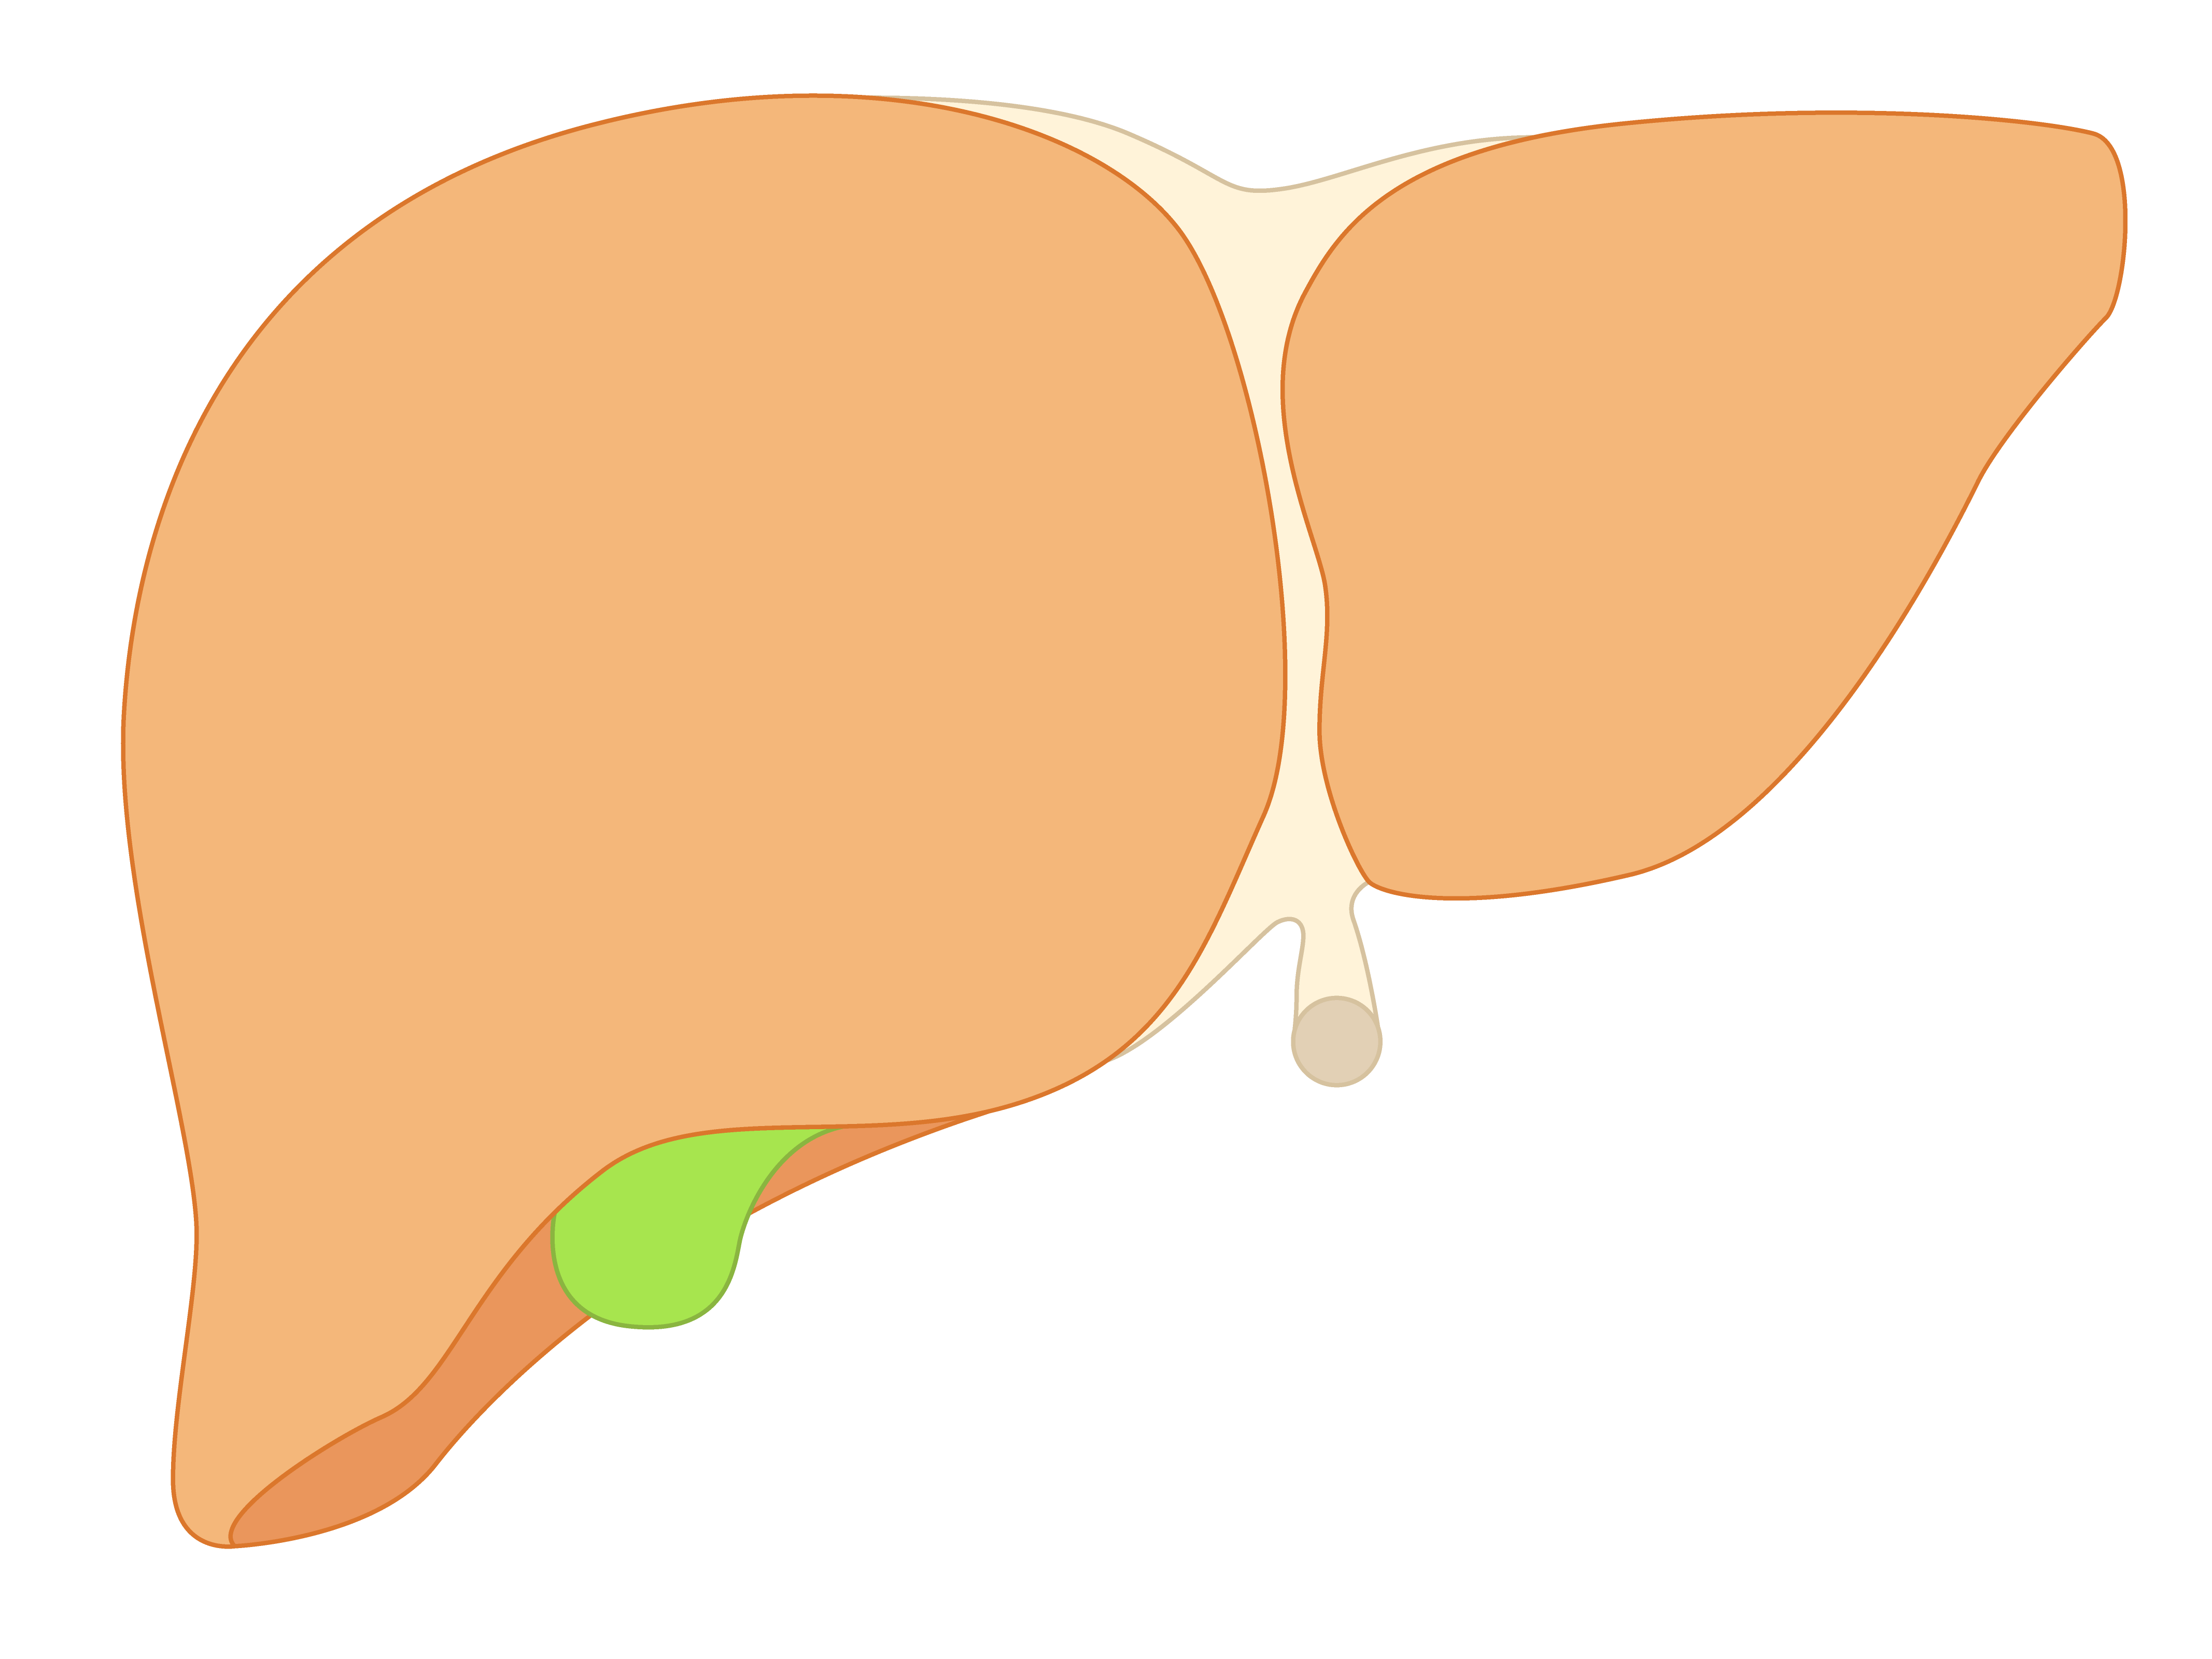
\includegraphics[height=200pt]{Figures/HealsyLiver.png}}
\newsavebox{\titleimagetwo}
\savebox{\titleimagetwo}{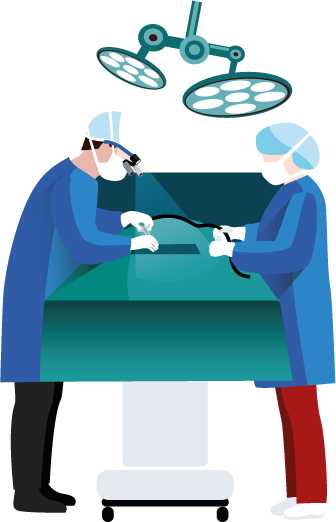
\includegraphics[height=200pt]{Figures/OR Team.png}}
\title[Захворювання печінки та їх лікування]{%
\setlength{\parindent}{0pt}%
  Захворювання печінки \par  та  їх лікування \par \vspace{1cm}
  \usebox{\titleimageone}
  \usebox{\titleimagetwo}}


\author[Відділ трансплантації та хірургії печінки]{Відділ трансплантації та хірургії печінки}
\publisher{\setlength{\parindent}{0pt}Національний інститут хірургії\parта трансплантології ім.О.О.Шалімова}


% Prints an epigraph and speaker in sans serif, all-caps type.
\newcommand{\openepigraph}[2]{%
  %\sffamily\fontsize{14}{16}\selectfont
  \begin{fullwidth}
  \sffamily\large
  \begin{doublespace}
  \noindent\allcaps{#1}\\% epigraph
  \noindent\allcaps{#2}% author
  \end{doublespace}
  \end{fullwidth}
}

% Inserts a blank page
\newcommand{\blankpage}{\newpage\hbox{}\thispagestyle{empty}\newpage}

\usepackage{units}

% Typesets the font size, leading, and measure in the form of 10/12x26 pc.
\newcommand{\measure}[3]{#1/#2$\times$\unit[#3]{pc}}

% Macros for typesetting the documentation
\newcommand{\hlred}[1]{\textcolor{Maroon}{#1}}% prints in red
\newcommand{\hangleft}[1]{\makebox[0pt][r]{#1}}
\newcommand{\hairsp}{\hspace{1pt}}% hair space
\newcommand{\hquad}{\hskip0.5em\relax}% half quad space
\newcommand{\TODO}{\textcolor{red}{\bf TODO!}\xspace}
\newcommand{\ie}{\textit{i.\hairsp{}e.}\xspace}
\newcommand{\eg}{\textit{e.\hairsp{}g.}\xspace}
\newcommand{\na}{\quad--}% used in tables for N/A cells
\providecommand{\XeLaTeX}{X\lower.5ex\hbox{\kern-0.15em\reflectbox{E}}\kern-0.1em\LaTeX}
\newcommand{\tXeLaTeX}{\XeLaTeX\index{XeLaTeX@\protect\XeLaTeX}}
% \index{\texttt{\textbackslash xyz}@\hangleft{\texttt{\textbackslash}}\texttt{xyz}}
\newcommand{\tuftebs}{\symbol{'134}}% a backslash in tt type in OT1/T1
\newcommand{\doccmdnoindex}[2][]{\texttt{\tuftebs#2}}% command name -- adds backslash automatically (and doesn't add cmd to the index)
\newcommand{\doccmddef}[2][]{%
  \hlred{\texttt{\tuftebs#2}}\label{cmd:#2}%
  \ifthenelse{\isempty{#1}}%
    {% add the command to the index
      \index{#2 command@\protect\hangleft{\texttt{\tuftebs}}\texttt{#2}}% command name
    }%
    {% add the command and package to the index
      \index{#2 command@\protect\hangleft{\texttt{\tuftebs}}\texttt{#2} (\texttt{#1} package)}% command name
      \index{#1 package@\texttt{#1} package}\index{packages!#1@\texttt{#1}}% package name
    }%
}% command name -- adds backslash automatically
\newcommand{\doccmd}[2][]{%
  \texttt{\tuftebs#2}%
  \ifthenelse{\isempty{#1}}%
    {% add the command to the index
      \index{#2 command@\protect\hangleft{\texttt{\tuftebs}}\texttt{#2}}% command name
    }%
    {% add the command and package to the index
      \index{#2 command@\protect\hangleft{\texttt{\tuftebs}}\texttt{#2} (\texttt{#1} package)}% command name
      \index{#1 package@\texttt{#1} package}\index{packages!#1@\texttt{#1}}% package name
    }%
}% command name -- adds backslash automatically
\newcommand{\docopt}[1]{\ensuremath{\langle}\textrm{\textit{#1}}\ensuremath{\rangle}}% optional command argument
\newcommand{\docarg}[1]{\textrm{\textit{#1}}}% (required) command argument
\newenvironment{docspec}{\begin{quotation}\ttfamily\parskip0pt\parindent0pt\ignorespaces}{\end{quotation}}% command specification environment
\newcommand{\docenv}[1]{\texttt{#1}\index{#1 environment@\texttt{#1} environment}\index{environments!#1@\texttt{#1}}}% environment name
\newcommand{\docenvdef}[1]{\hlred{\texttt{#1}}\label{env:#1}\index{#1 environment@\texttt{#1} environment}\index{environments!#1@\texttt{#1}}}% environment name
\newcommand{\docpkg}[1]{\texttt{#1}\index{#1 package@\texttt{#1} package}\index{packages!#1@\texttt{#1}}}% package name
\newcommand{\doccls}[1]{\texttt{#1}}% document class name
\newcommand{\docclsopt}[1]{\texttt{#1}\index{#1 class option@\texttt{#1} class option}\index{class options!#1@\texttt{#1}}}% document class option name
\newcommand{\docclsoptdef}[1]{\hlred{\texttt{#1}}\label{clsopt:#1}\index{#1 class option@\texttt{#1} class option}\index{class options!#1@\texttt{#1}}}% document class option name defined
\newcommand{\docmsg}[2]{\bigskip\begin{fullwidth}\noindent\ttfamily#1\end{fullwidth}\medskip\par\noindent#2}
\newcommand{\docfilehook}[2]{\texttt{#1}\index{file hooks!#2}\index{#1@\texttt{#1}}}
\newcommand{\doccounter}[1]{\texttt{#1}\index{#1 counter@\texttt{#1} counter}}

% Generates the index
\usepackage{makeidx}
\makeindex

\begin{document}

% Front matter
\frontmatter

% r.1 blank page
%\blankpage

% r.3 full title page
\maketitle

% v.2 epigraphs
% v.4 copyright page
\newpage
\begin{fullwidth}
~\vfill
\thispagestyle{empty}
\setlength{\parindent}{0pt}
\setlength{\parskip}{\baselineskip}
Copyright \copyright\ \the\year\ \thanklessauthor

\par\smallcaps{Розробник: \thanklesspublisher}

\end{fullwidth}

\newpage\thispagestyle{empty}

\chapter*{Попередження}

Цей довідник призначений для \textcolor{red}{початкового ознайомлення}   пацієнтів з основними захворюваннями печінки та принципами їх лікування. Довідник містить достовірну але спрощену для сприйняття ознайомчу інформацію з медичної тематики та \textcolor{red}{не може бути використаний, як інструкція до лікування} або як заміна консультації лікаря.

Будь-які призначення або вибір тактики лікування  повинен проводити \textcolor{red}{тільки відповідний фахівець охорони здоров'я}. 

Самостійне лікування, зміна чи невиконання призначеннь лікаря,  інтерпретація результатів  аналізів та медичних дослідженнь пацієнтом без спеціальних медичних знаннь може призводити до погіршання результату лікування, втрати лікувальних можливостей та погіршання стану здоров'я    

\vfill

\tableofcontents

\mainmatter

\chapter{Будова та функція печінки}

\section{Що таке печінка?}

Печінка - це найбільший орган черевної порожнини, «біохімічна лабораторія» організму, яка виконує велику кількість життєво важливих для людини функцій (Мал. \ref{fig:healthyliver}).



\begin{marginfigure}%
  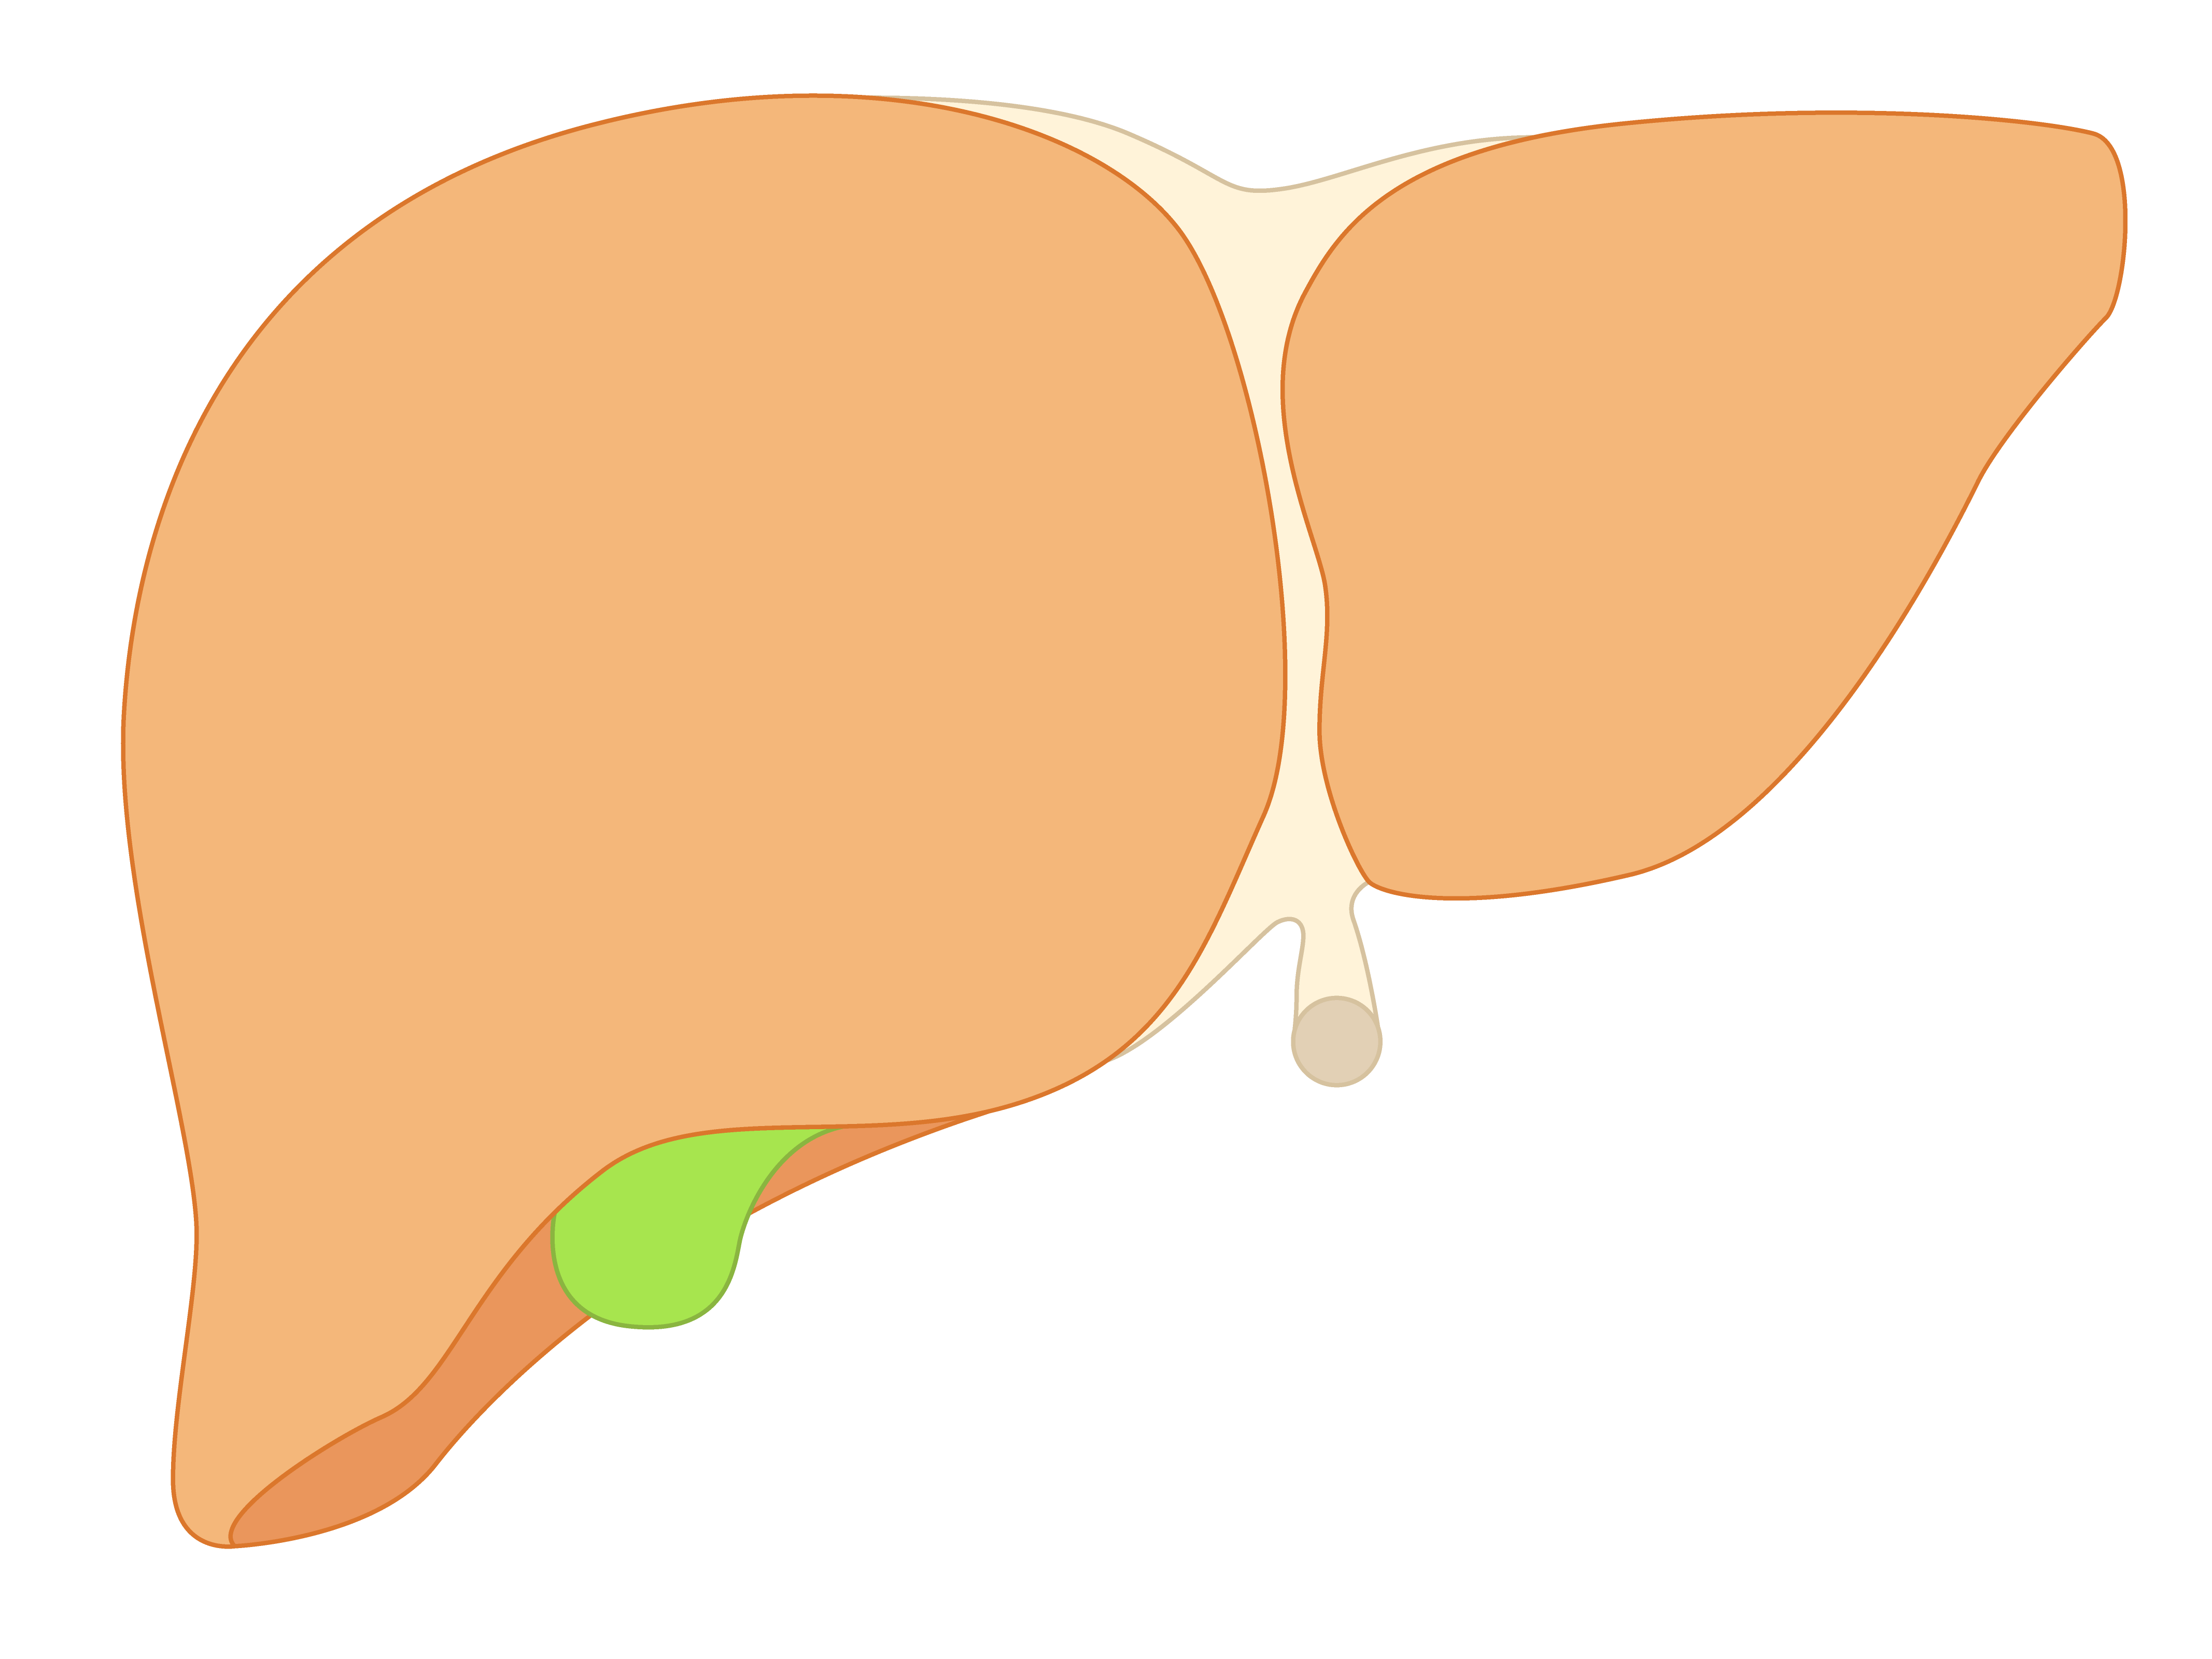
\includegraphics[width=\linewidth]{Figures/HealsyLiver.png}
  \caption{Схематичний зовнішній вигляд печінки}
  \label{fig:healthyliver}
\end{marginfigure}

\section{Де розташована печінка?}

Печінка знаходиться у правій верхній частині живота, під діафрагмою та захищена реберною дугою. 

\begin{marginfigure}[10pt]%
  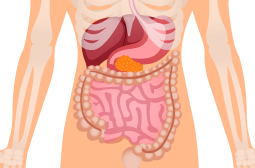
\includegraphics[width=\linewidth]{Figures/LiverRelation.png}
  \caption{Положення печінки в тілі людини}
  \label{fig:liverrelation}
\end{marginfigure}

Печінка розташована (Мал. \ref{fig:liverrelation}) поруч із шлунком, підшлунковою залозою, товстим кішківником, правою ниркою та наднирником і магістральними судинами організму — абдомінальними частинами аорти та нижньої порожнистої вени. \sidenote[][20pt]{Ця інформація важлива для розуміння принципу оперативного лікування новоутвореннь печінки, які виходять за межі органа}

\section{Яка внутрішня будова печінки?}

Печінка вкрай складний орган та має унікальну подвійну систему кровопостачання. Як і більшість органів в тілі людини, печінка отримує артеріальну кров з аорти по гілках печінкової артерії. Ця кров живить строму — каркас печінки, до якого входять жовчі протоки та судини в середині органа. Окрім того, на відміну від інших органів, печінка отримує по системі ворітної (портальної) вени ще й венозну кров від усіх непарних органів черевної порожнини, а саме шлунку, тонкого та товстого кішківника, селезінки та підшлункової залози (мал. \ref{fig:livervasculature}). Це дозволяє печінці переробляти поживні речовини, що всмоктуються в кров з кішківника під час процесу травлення. \sidenote[][10pt]{Розуміння кровопостачання печінки та системи портального кровотоку необхідне для усвідомлення принципу лікування пухлин печінки та портальної гіпертензії} 

Відтікає кров від печінки по системі печінкових вен, які впадають в нижню порожнисту вену поруч із правим передсердям. 


\newpage

\begin{figure*}[h]
  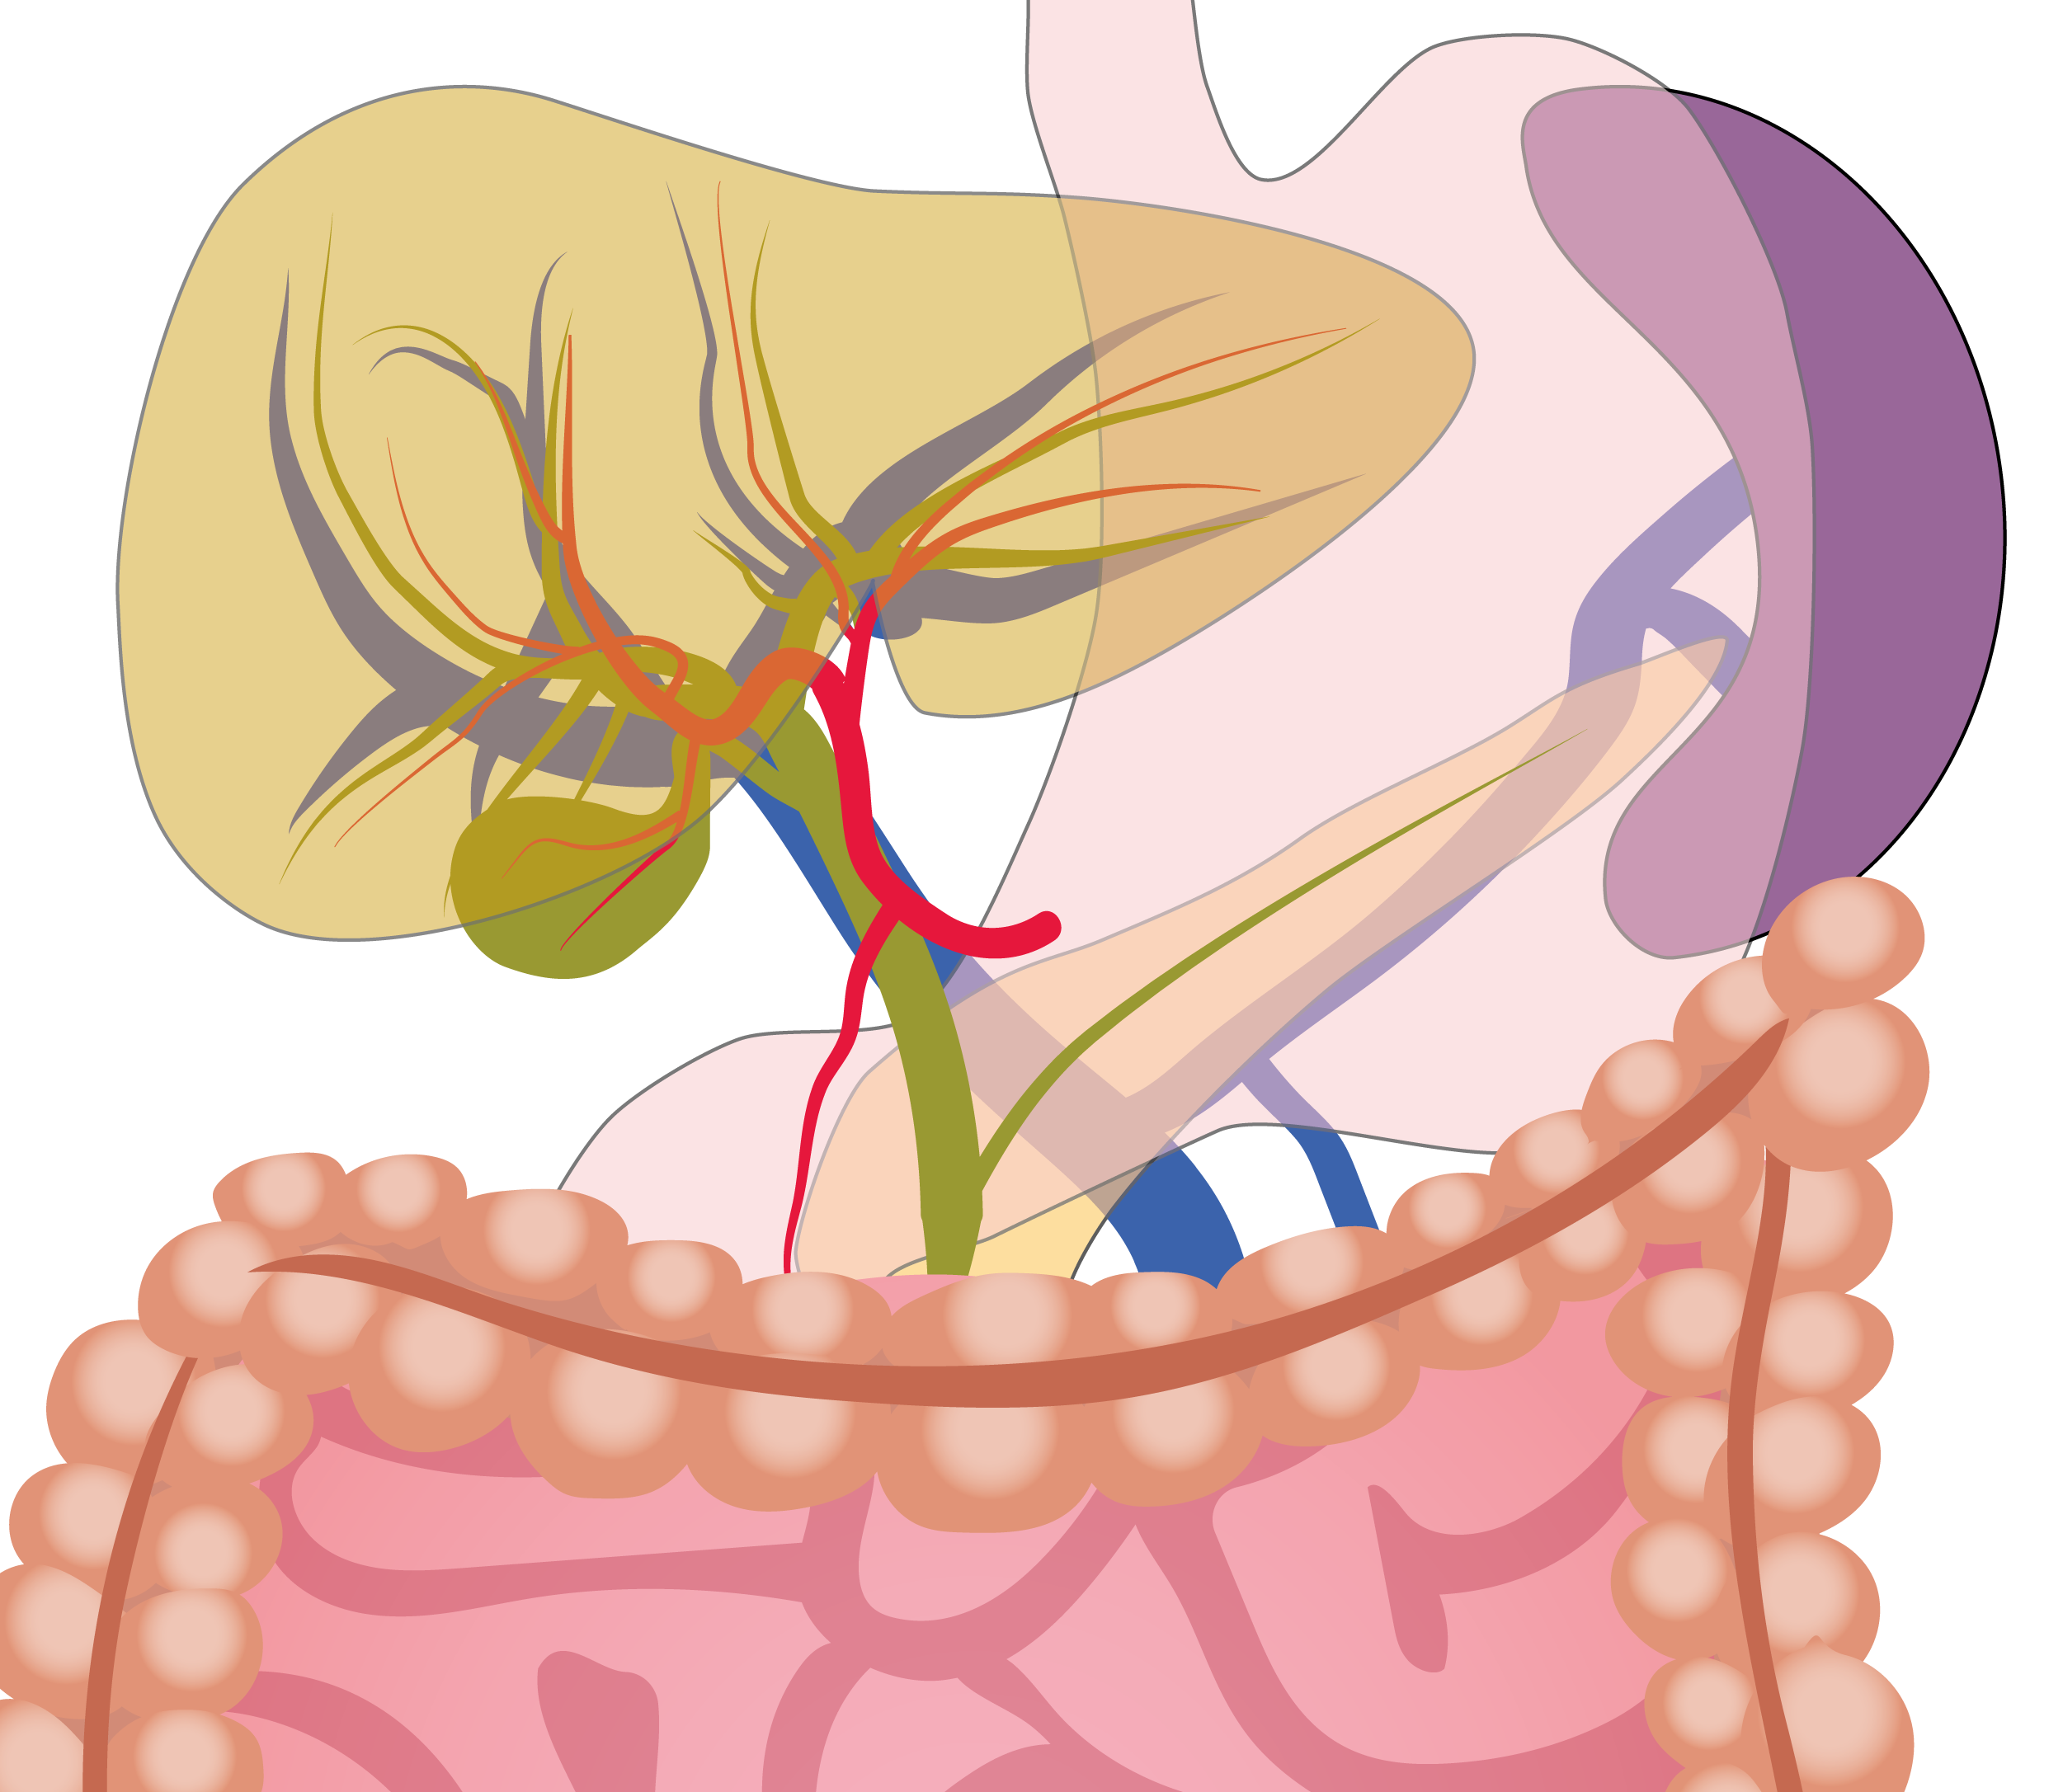
\includegraphics[width=\linewidth]{Figures/Liver vasculature_Liver and guts.png}%
  \caption{Кровопостачання печінки}%
  \label{fig:livervasculature}%
\end{figure*}

В середині печінки її судини та жовчні протоки поділяються, подібно до поділу стовбура дерева на гілки та утворюють судинно-секреторні пучки, що мають назву глісонових ніжок. Кожна з таких гілок (глісонова ніжка) має свою «крону листя» - окрему ділянку тканини печінки, яку вона кровопостачає та з якої відводить жовч.  Така ділянка тканини печінки має назву сегмент печінки (мал. \ref{fig:liversegments}). Всього печінка поділяється на вісім сегментів. 

\begin{marginfigure}%
  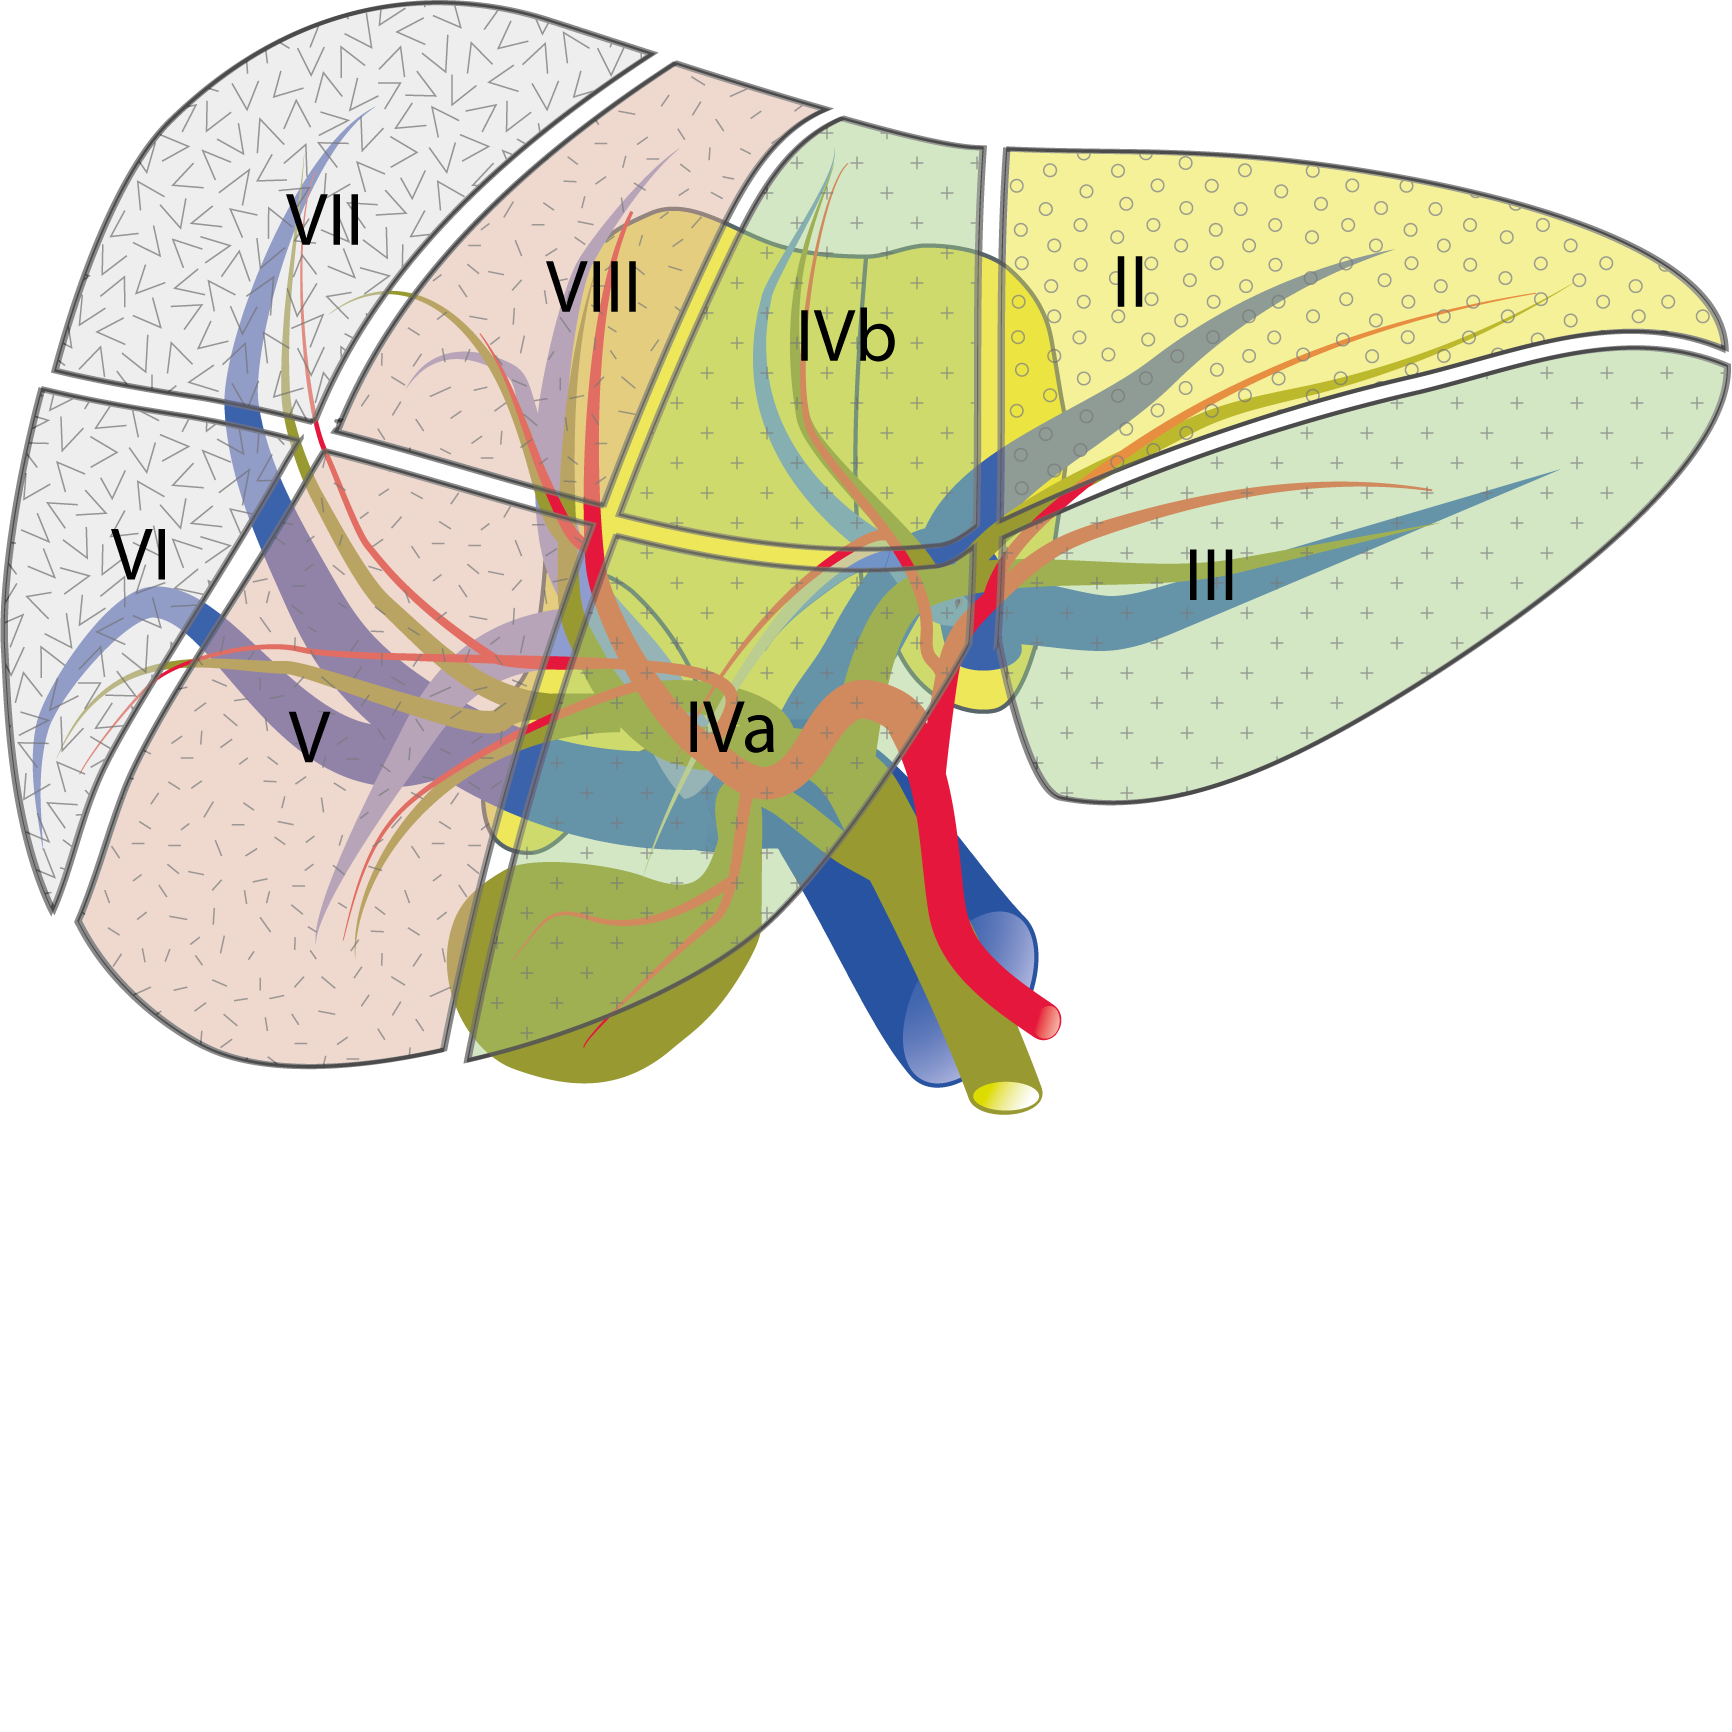
\includegraphics[width=\linewidth]{Figures/LiverSegments.png}
  \caption{Поділ печінки на сегменти}
  \label{fig:liversegments}
\end{marginfigure}

\begin{figure}
  \includegraphics[width=\linewidth]{Figures/Liver architecture-02.png}
  \caption{Гістологічна будова печінки. \par Тканина печінки складається з: а) паренхіми -- впорядкованих клітин печіни гепатоцитів та б) строми -- пучків судин та жовчних протоків}
  \label{fig:liverarchitecture}
\end{figure}

Сучасна хірургія печінки базується на видаленні новоутвореннь в межах окремих сегменітв печінки. Це більш безпечно, так як при цьому вся залишкова паренхіма має адекватне кровопостачання. Також це підвищує радикальність видалення пухлини.

\newpage
\section{Що таке жовч? Як вона виводиться?}

\begin{marginfigure}[-30pt]%
  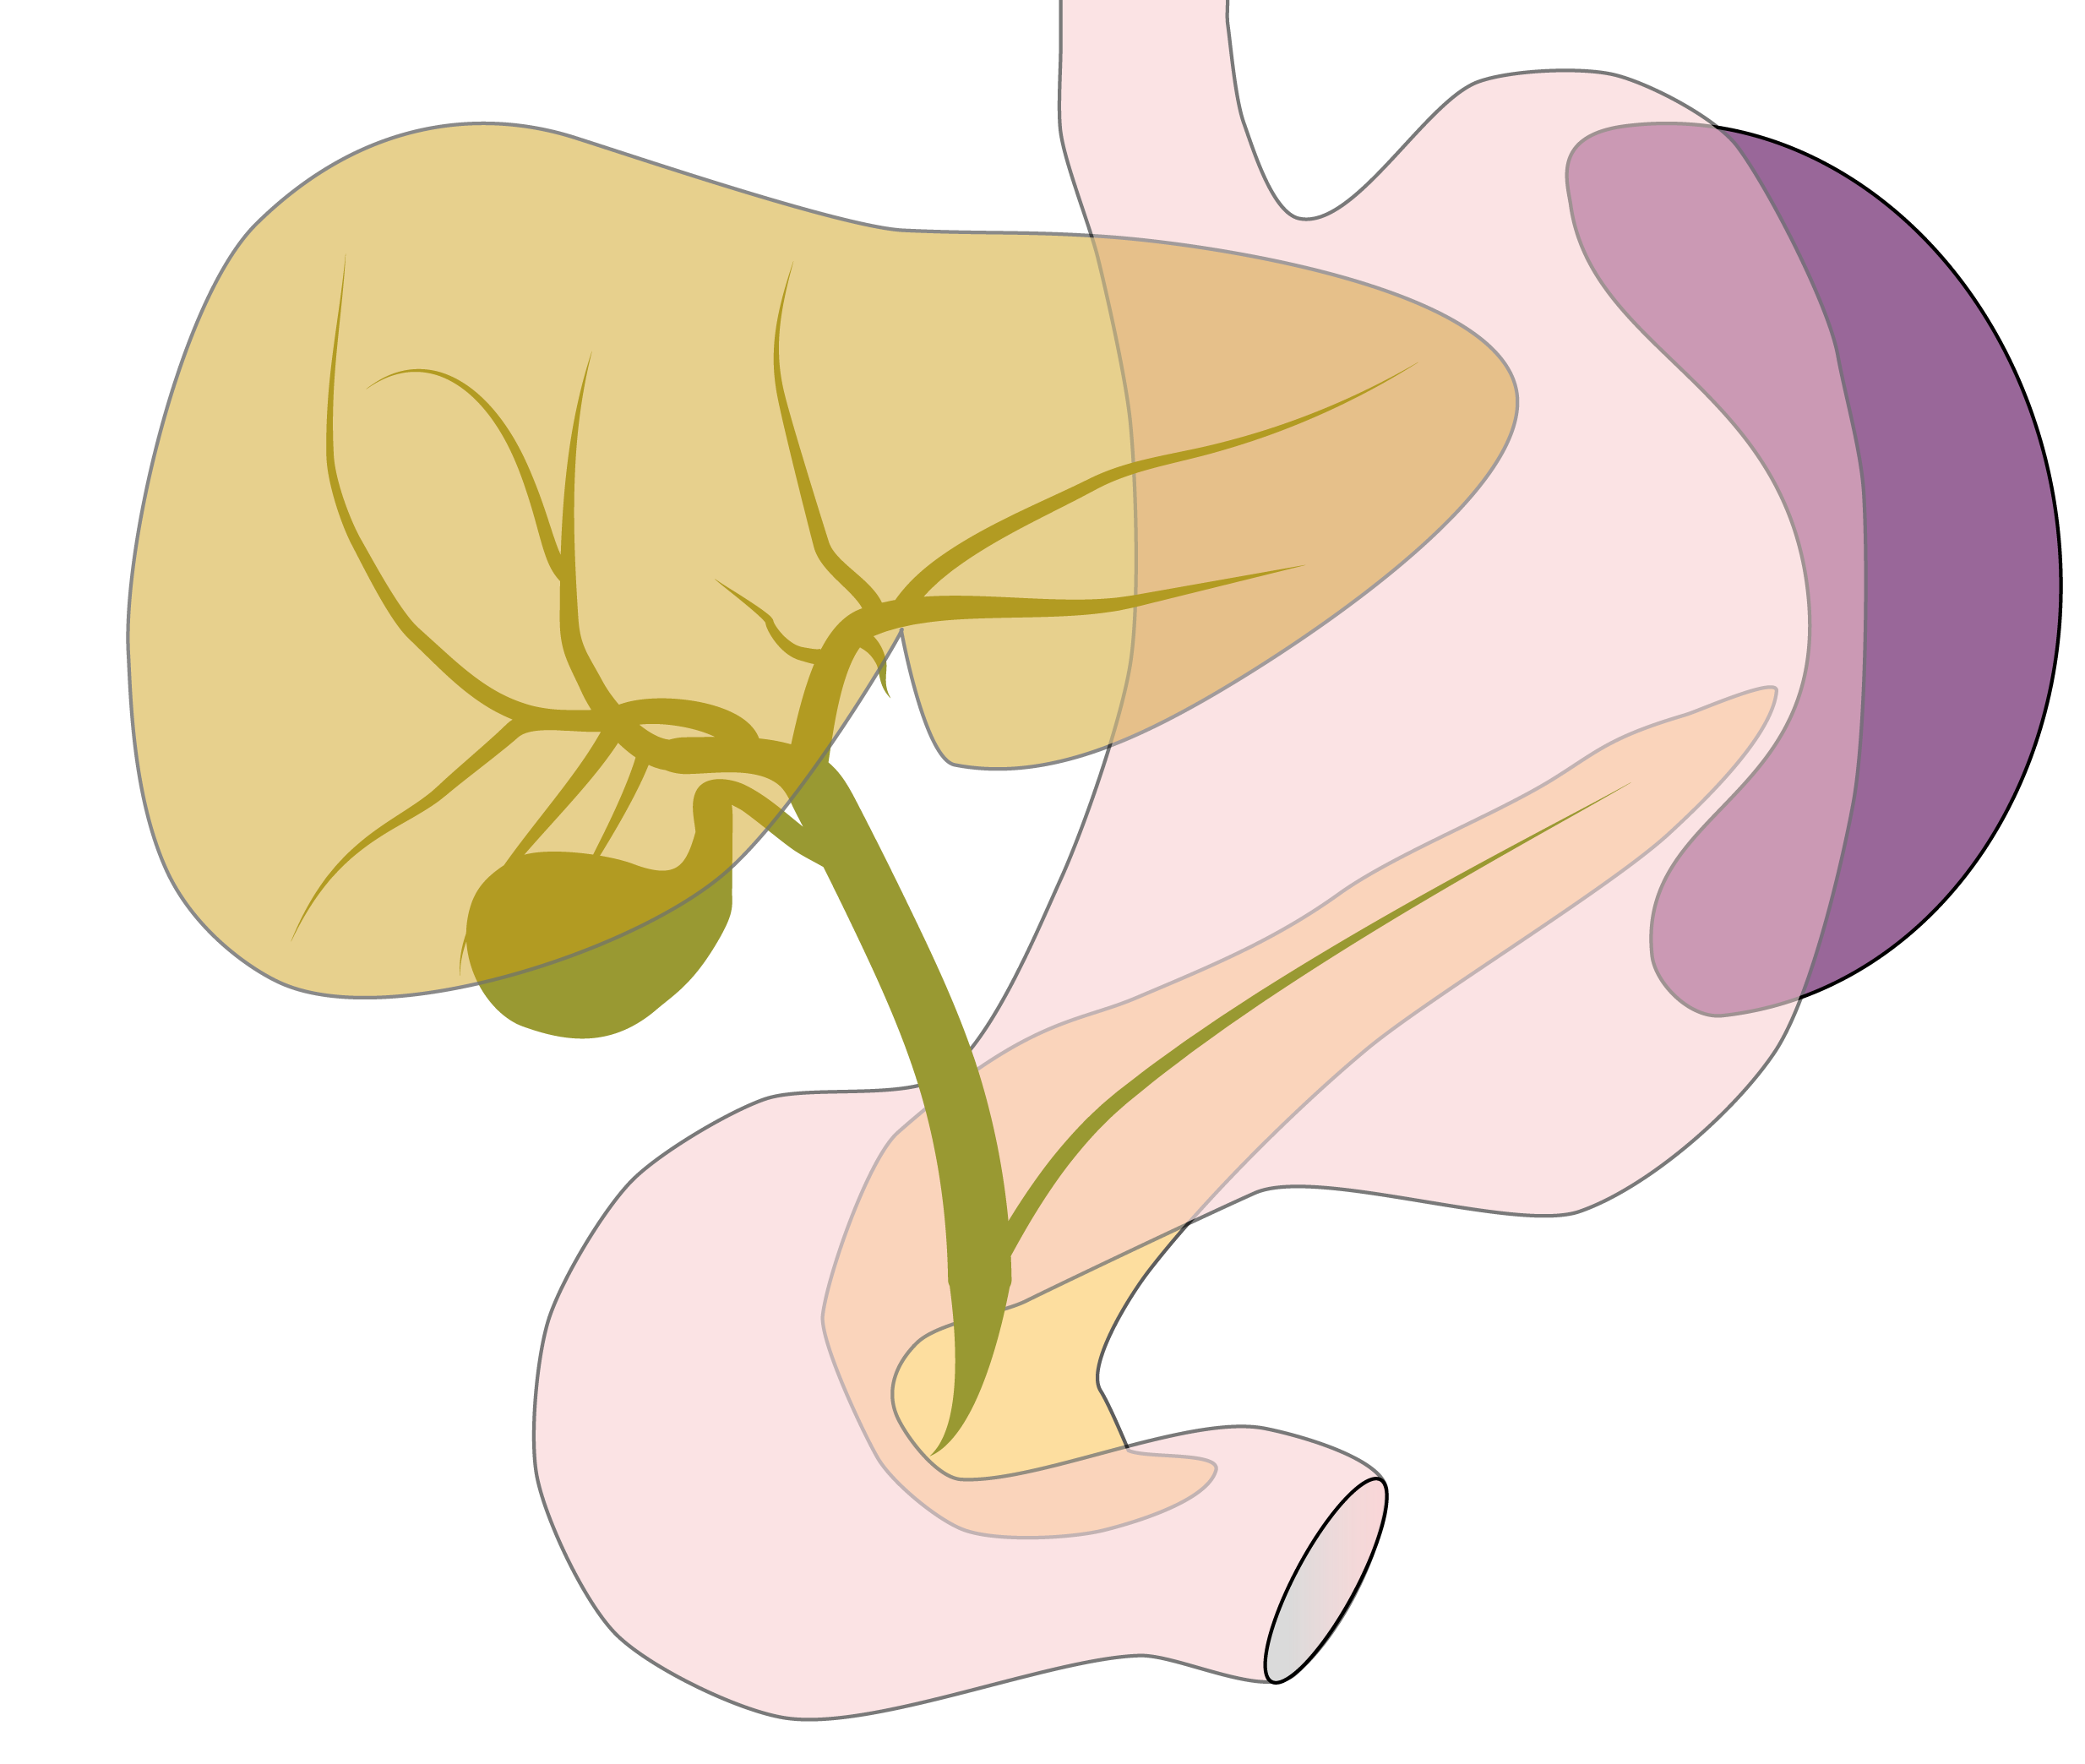
\includegraphics[width=\linewidth]{Figures/BileDucts_Focus on liver.png}
  \caption{Жовчні протоки печінки}
  \label{fig:bileducts}
\end{marginfigure}

Жовч — це необхідна для процесу травлення фізиологічна рідина, яку виділяють клітини печінки. По системі жовчних проток жовч потрапляє з печінки в кишківник.  Жовчні шляхи починаються в середині печінки у вигляді мікрокапелярів, потім об’єднуються та формують протоки все більшого діаметру. З печінки виходить одна велика протока, яка після об’єднання з протокою жовчного міхура, крізь тканину підшлункової залози потрапляє в дванадцятипалу кишку. \sidenote[][50pt]{Знання про систему жовчовідтоку необхідне для усвідомлення принципу лікування захворюваннь, що перебігають із механічною жовтяницею}


\section{Що таке жовчний міхур?}

Жовчний міхур це орган, який є частиною жовчовивідних шляхів. Жовчний міхур виконує функцію резервуара, де зберігається невелика кількість концентрованої жовчі між прийомами їжі. Після потрапляння їжі в травний канал жовчний міхур скорочується та викидає жовч в кишку, що полегшує травлення. Жовчний міхур не виробляє а лише зберігає малу частину жовчі (2-3\% від кількості яку печінка виділяє за добу). За його відсутності цю роль частково беруть на себе жовчні шляхи та печінка.

\begin{marginfigure}[50pt]%
  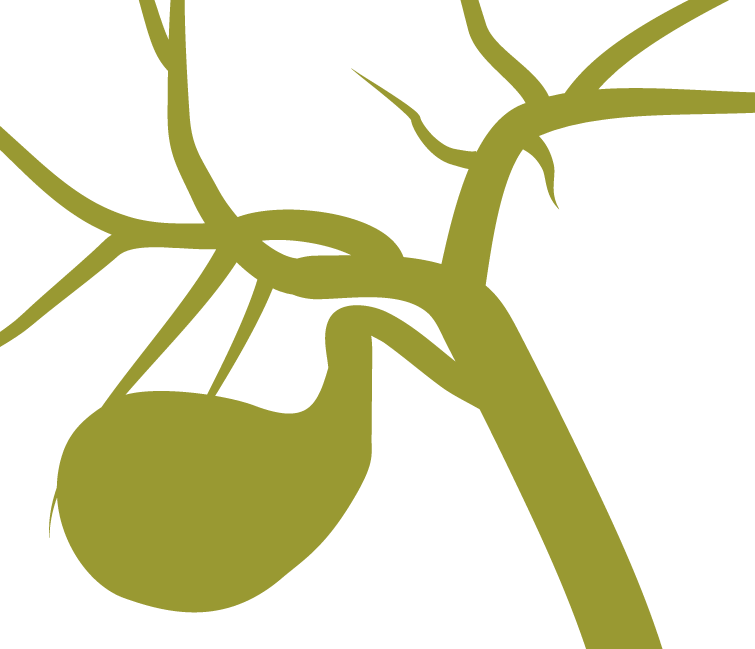
\includegraphics[width=\linewidth]{Figures/Goalbladder_Focus on hilum.png}
  \caption{Жовчий міхур - резервуар, який тимчасово зберігає невелику кількість жовчі}
  \label{fig:goalbladder}
\end{marginfigure}

\section{Які ще функції, окрім виділення жовчі, має печінка?}

Печінка - універсальна біохімічна лабораторія організму в якій відбувається метаболізм жирів, білків та вуглеводнів. Вона забезпечує організм енергією завдяки синтезу глюкози, яка є основною «енергетичною валютою».  Також  печінка зберігає запас глікогена - речовини, що за потреби швидко перетворюється на глюкозу. Печінка синтезує велику кількість білків плазми крові, таких, як альбумін та фактори згортання та деякі гормони. Також печінка є ключовим органом іммунної системи - вона є імунним бар’єром між портальною кров’ю з кішківника та системним кровотоком, а також тут синтезується 80-90\% імунних білків. Окрім цього, печінка відповідальна за знешкодження токсинів, які потрапляють в організм з їжею чи іншим шляхом. \sidenote[][30pt]{Інформація про печінкові функції та їх порушення необхідна для розуміння проявів її захворюваннь та/чи адекватної оцінки ризиків ускладненнь оперативного втручання}

\section{До чого призводить порушення функції печінки?}
Печінка є органом, що має велику здібність до регенерації та відновлення. Проте при вичерпанні цього ресурсу внаслідок захворювання функція її може порушуватись. \sidenote[][30pt]{Для визначення функціонального стану печінки найбільш часто використовують розширений біохімічний аналіз крові та коагулограмму. За результатами цих дослідженнь спеціаліст може зробити висновки про наявність чи відсутність порушення функції печінки. 

Окрім цього існує велика кількість спеціальних функціональних тестів, таких як  фіброеластографія, ICG-тест та ін. 

Про необхідність саме вам проходити той чи інший тест ви можете запитати у лікаря під час консультації}

Порушення функції печінки до таких проявів, як:
\begin{itemize}
  \item Жовтяниця - патологічний стан, при якому печінка не здатна захватити з крові та вивести із жовччю білірубін (токсичний пігмент, кінцевий продукт розпаду гемоглобіну), що призводить до пожовтіння всіх тканин організму та інтоксикації
  \item Порушення синтезу факторів згортання плазми, яке призводить до погіршання згортання крові та ризику спонтанних кровотеч та крововиливів
  \item Порушення синтезу альбуміну - головного білка-переносчика плазми крові, що призводить до зниження онкотичного тиску крові, набряклості тканей та продукції асциту (скупчення рідини в черевній порожнині)
  \item Печінкова енцефалопатія - ураження головного мозку токсинами кишкового походження через порушення їх знешкодження в печінці (сонливість, неуважність, роздратованість, дезорієнтованість та сповільнення темпу мови)
  \item Інфекції та септичні стани внаслідок ураження імунітету
\end{itemize}

\section{\LARGE{Що мені варто запам'ятати з цього розділу?}}



\begin{tcolorbox}[width=\textwidth,colback={YellowGreen},colbacktitle=yellow,coltitle=blue]    
\allcaps{Печінка - життєвоважливий орган, який має складну анатомічну будову та велику кількість необхідних для організма функцій.}
\end{tcolorbox}    
\begin{marginfigure}%
  
\includegraphics[width=\linewidth]{Figures/Exclamation_mark.png}
\end{marginfigure}
\begin{tcolorbox}[width=\textwidth,colback={Goldenrod},colbacktitle=yellow,coltitle=blue]   
\allcaps{Жовчний міхур є лише додатковою частиною жовчовивідних шляхів, яка відіграє допоміжну функцію в процесі виведення жовчі.}
\end{tcolorbox}    

\chapter{Захворювання печінки}

\section{Які існують захворювання печінки?}

Існує велика кількість патології печінки, яку умовно можна розділити на \textit{дифузну} та вогнищеву. \sidenote[][40pt]{Хвороби печінки та їх лікування вивчає окрема наукова галузь медицини - гепатологія. }

При вогнищевій патології уражується частнина органа. До вогнищевої патології відносяться злоякісні та доброякісні пухлини, абсцеси, кістозна патологія та ін.

При дифузній патології внаслідок хронічного запалення (або дії іншого уражуючого фактору) пошкоджується вся паренхіма (тканина) органу. До дифузної патології відносяться цироз, фіброз, жировий гепатоз, амілоїдоз та ін.

\begin{figure}
  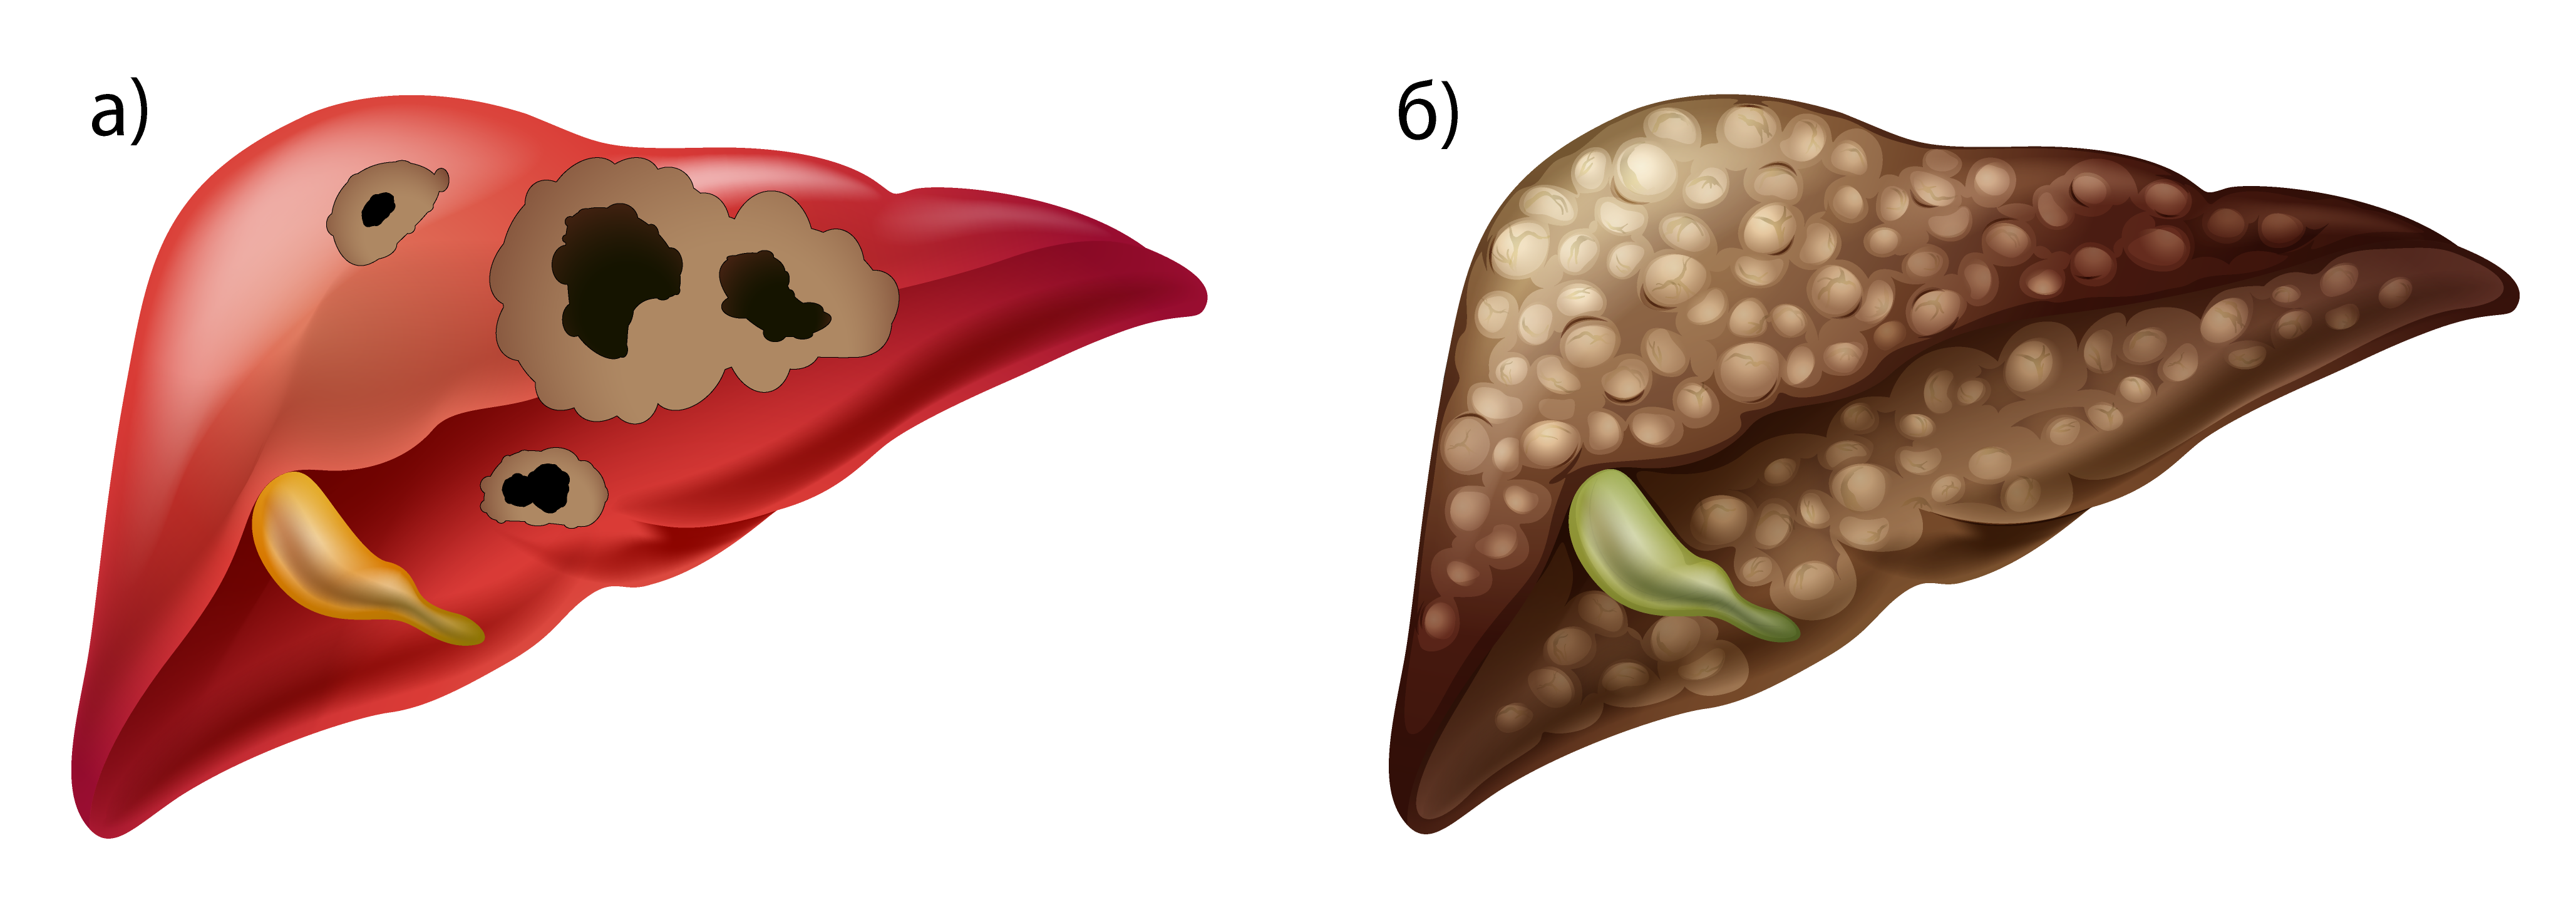
\includegraphics{Figures/Liver diseases_Diffuse and Nodular.png}
%  \checkparity This is an \pageparity\ page.%
  \caption{Патологія печінки. а) вогнищева патологія -- пухлина печінки, б) дифузна патологія -- цироз печінки }
  \label{fig:textfig}
  %\zsavepos{pos:textfig}
\end{figure}

\section{Які є види пухлин печінки?}

Пухлини печінки є основним видом її вогнищевої патології.
Розрізняють злоякісні та доброякісні пухлини печінки.

\begin{marginfigure}[20pt]%
  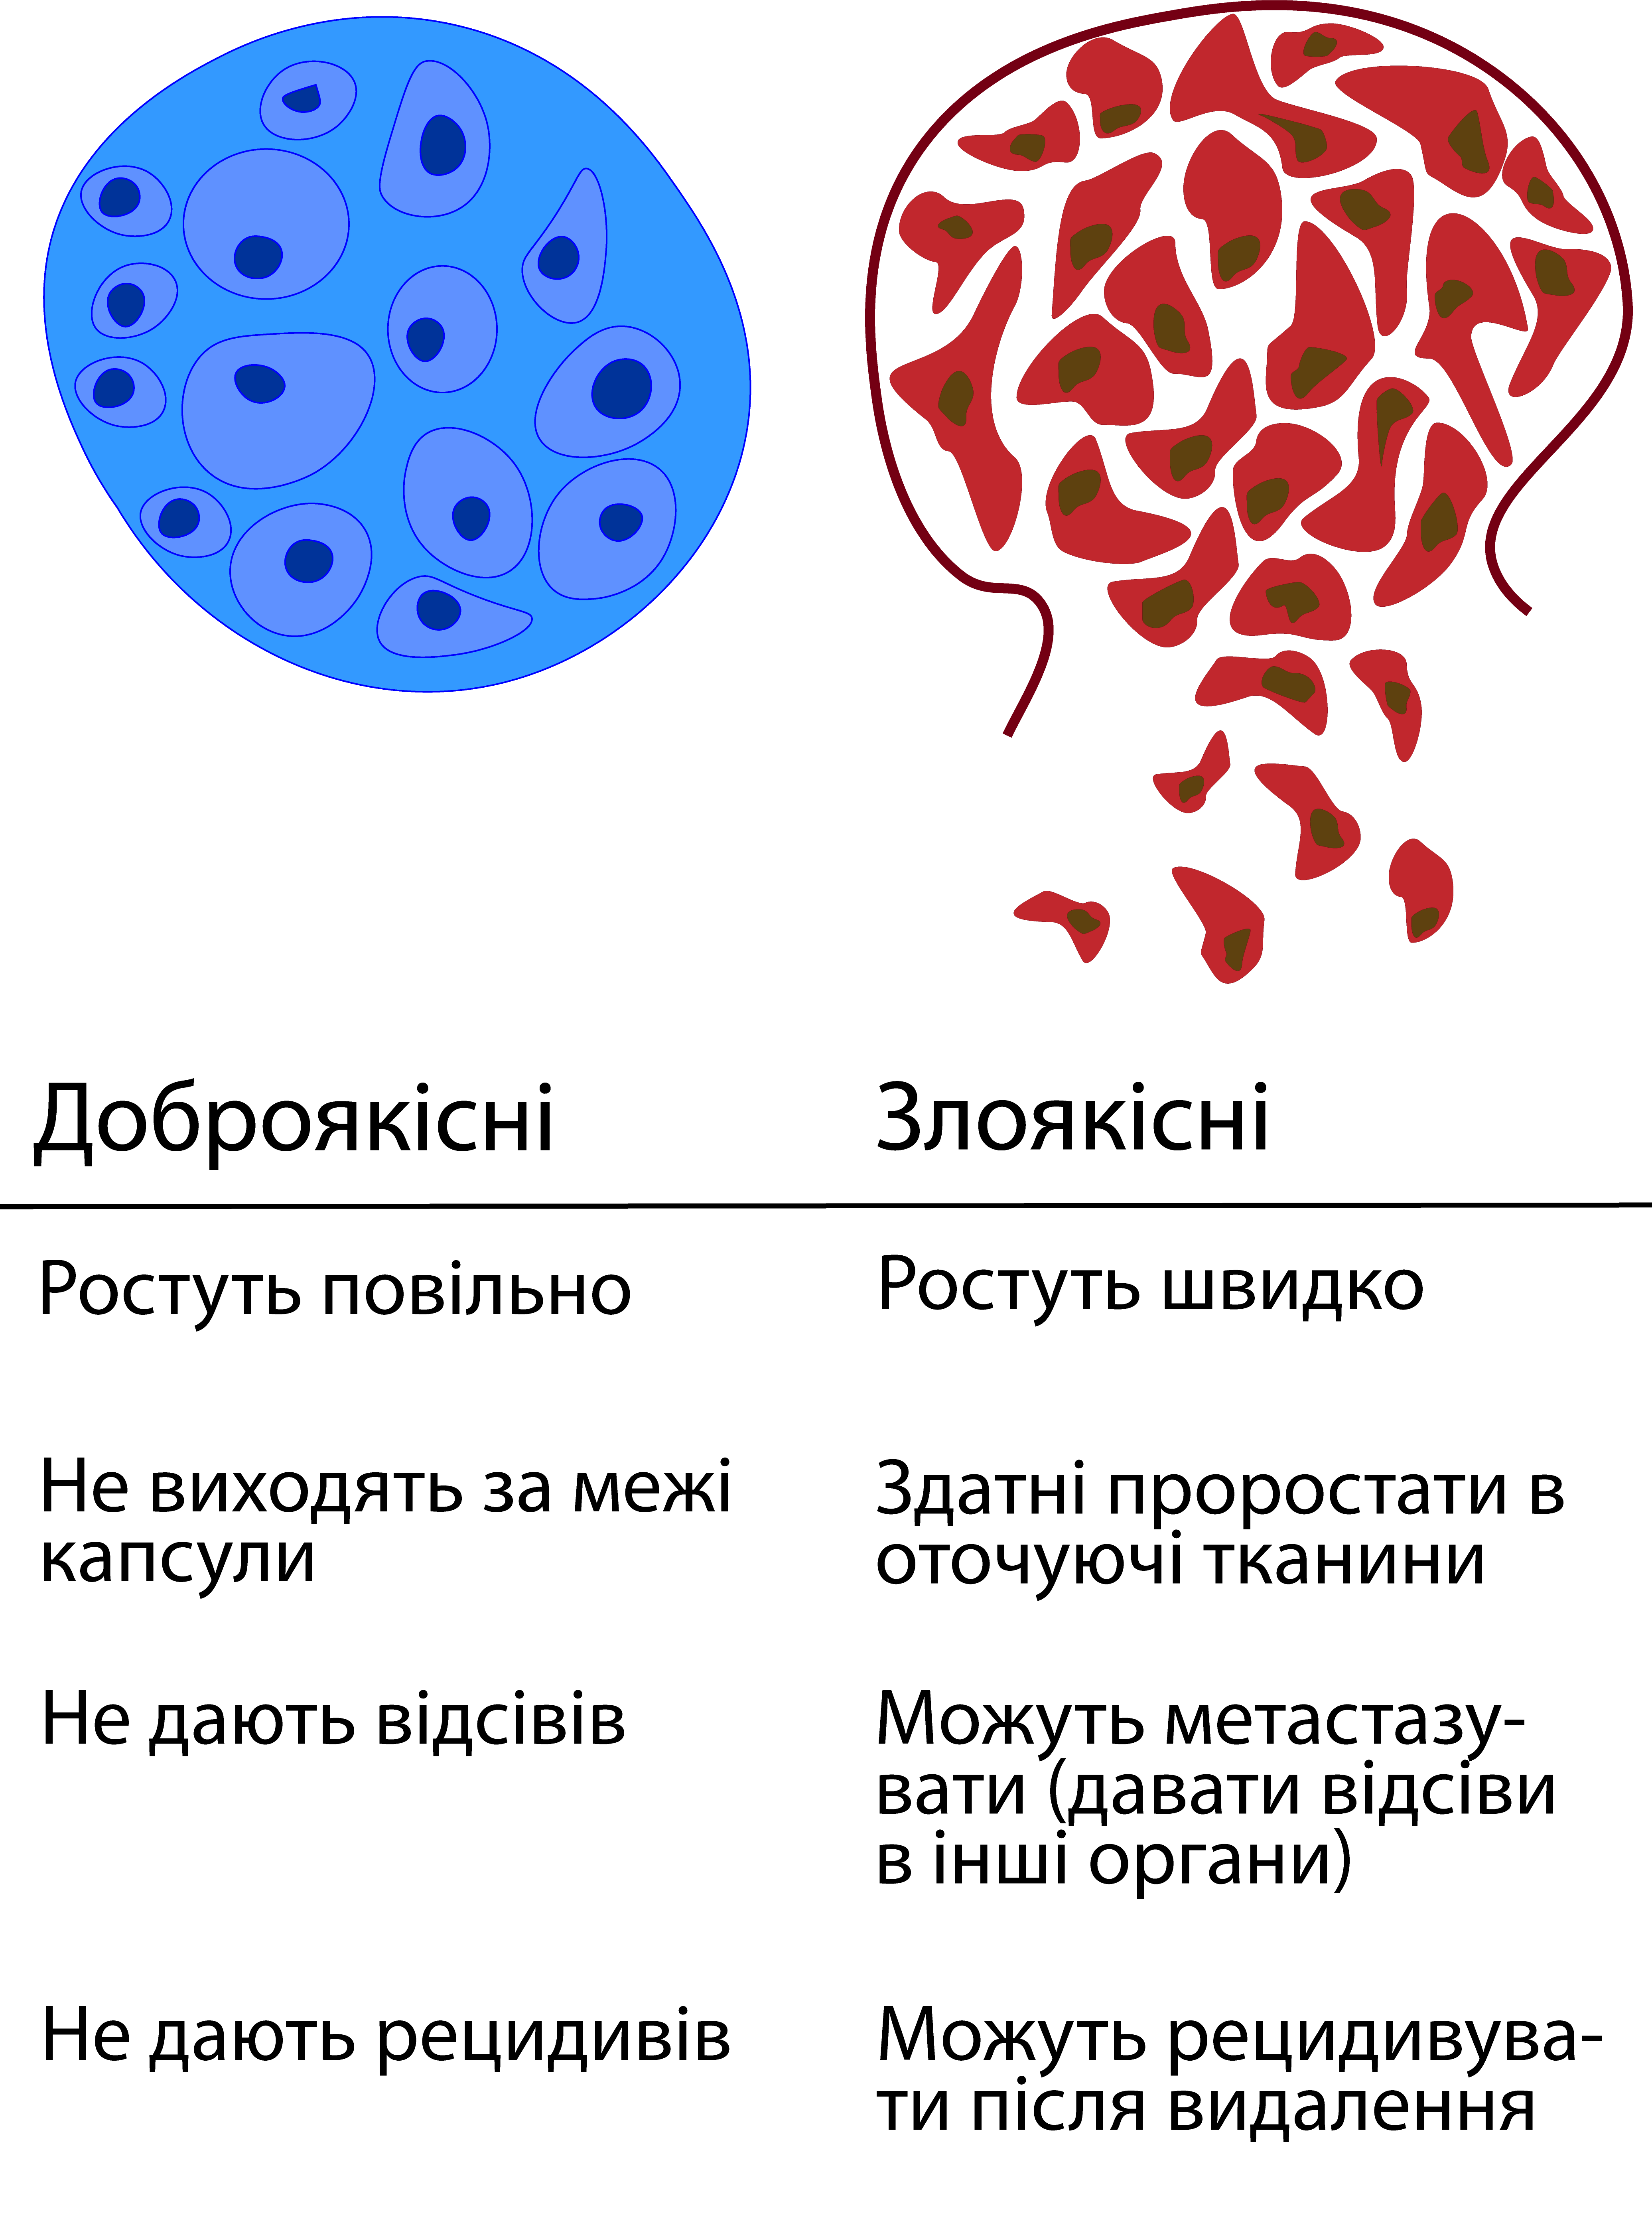
\includegraphics[width=\linewidth]{Figures/Benign vs malignant.png}
  \caption{Відмінності доброякісних та злоякісних пухлин}
  \label{fig:benignvsmalignant}
\end{marginfigure}

\section{Які є види злоякісних новоутвореннь печінки?}

Виділяють: 
\begin{enumerate}
    \item первинні пухлини печінки - ті що беруть своє первинне походження з клітин печінки або жовчних протоків, та
    \item вторинні (або метастатичні) - пухлини, які з’явились в печінці внаслідок міграції злоякісних клітин з інших органів
\end{enumerate} 

До первинних пухлин відносять такі захворювання:

\begin{itemize}
    \item Пухлини, що походять з гепатоцитів, клінтин тканини печінки
        \begin{itemize}
            \item гепатоцелюлярна карцинома (первинний рак печінки)
            \begin{marginfigure}[-10pt]%
                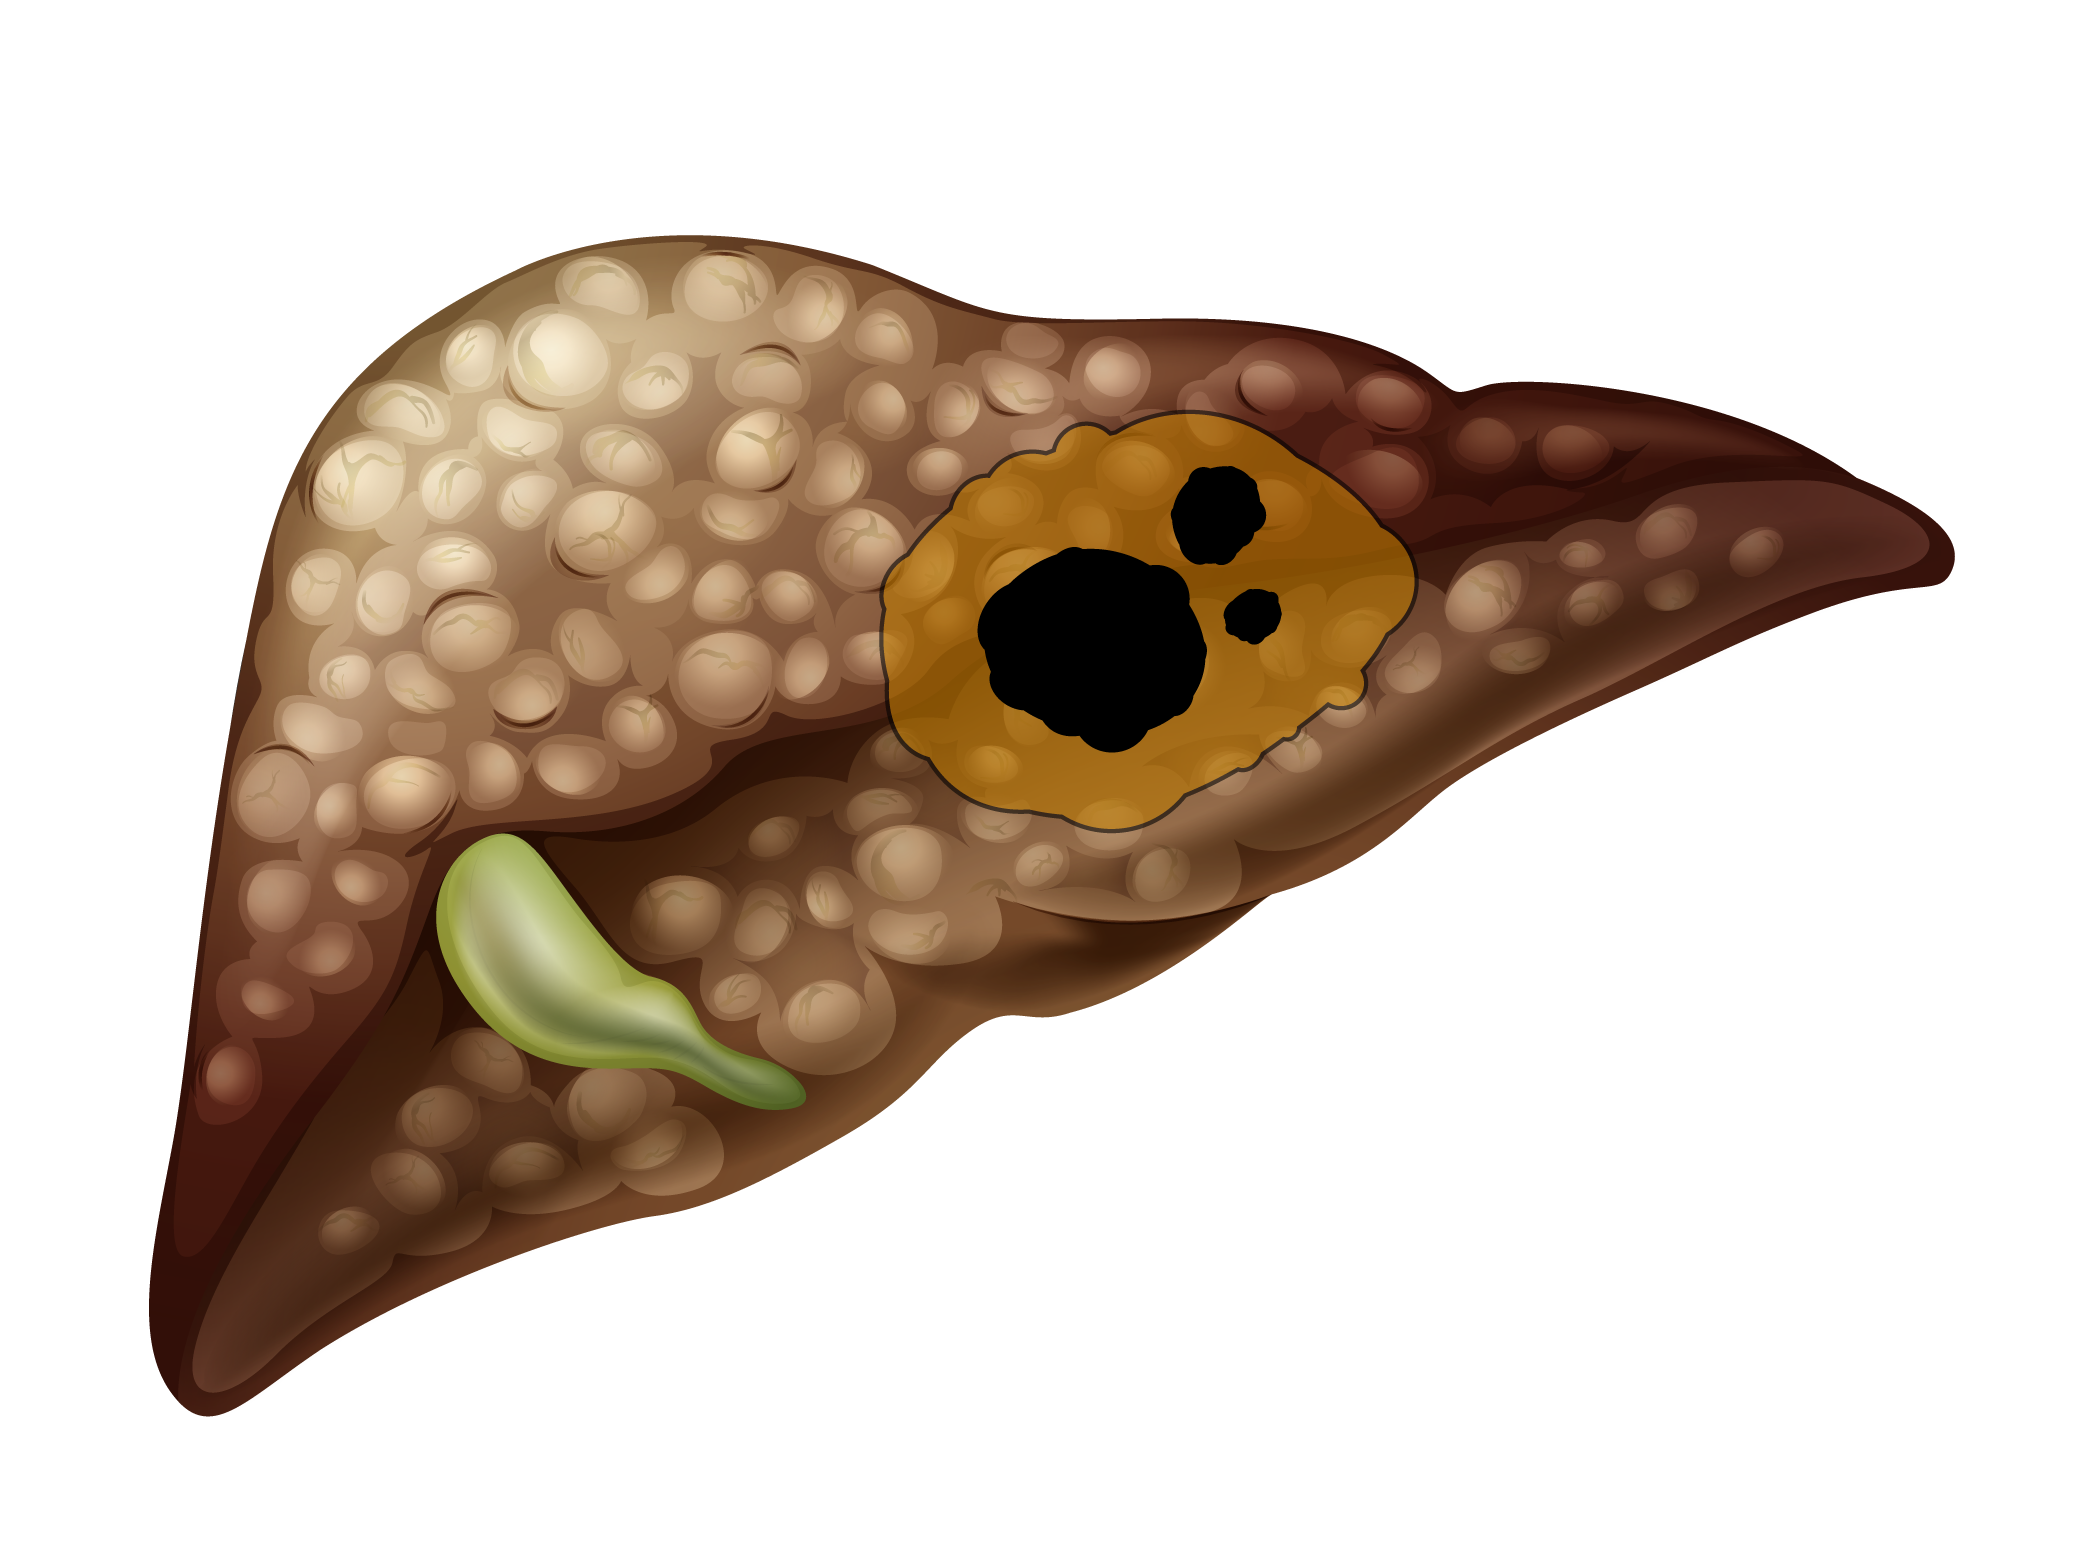
\includegraphics[width=\linewidth]{Figures/HCC.png}
                \caption{Гепацтоцеллюлярна карцинома (ГЦК). Первинний рак печінки -- пухлина, яка найчастіше виникає на фоні цирозу печінки}
                 \label{fig:hcc}
            \end{marginfigure}
            
            \item гепатобластома (особливий тип злоякісної пухлини печінки, що виникає переважно в дитячому віці)
            \item рак біліарного тракту (внутрішньопечінкова холангіокарцинома)
        \end{itemize}
    \item Пухлини, що походять біліарного тракту (жовчних протоків) 
        \begin{itemize}
            \item внутрішньопечінкова холангіокарцинома
            \item хіларна холангіокарцинома (рак розвилки жовчних шляхів або хвороба Клацкіна)
            \begin{marginfigure}[10pt]%
                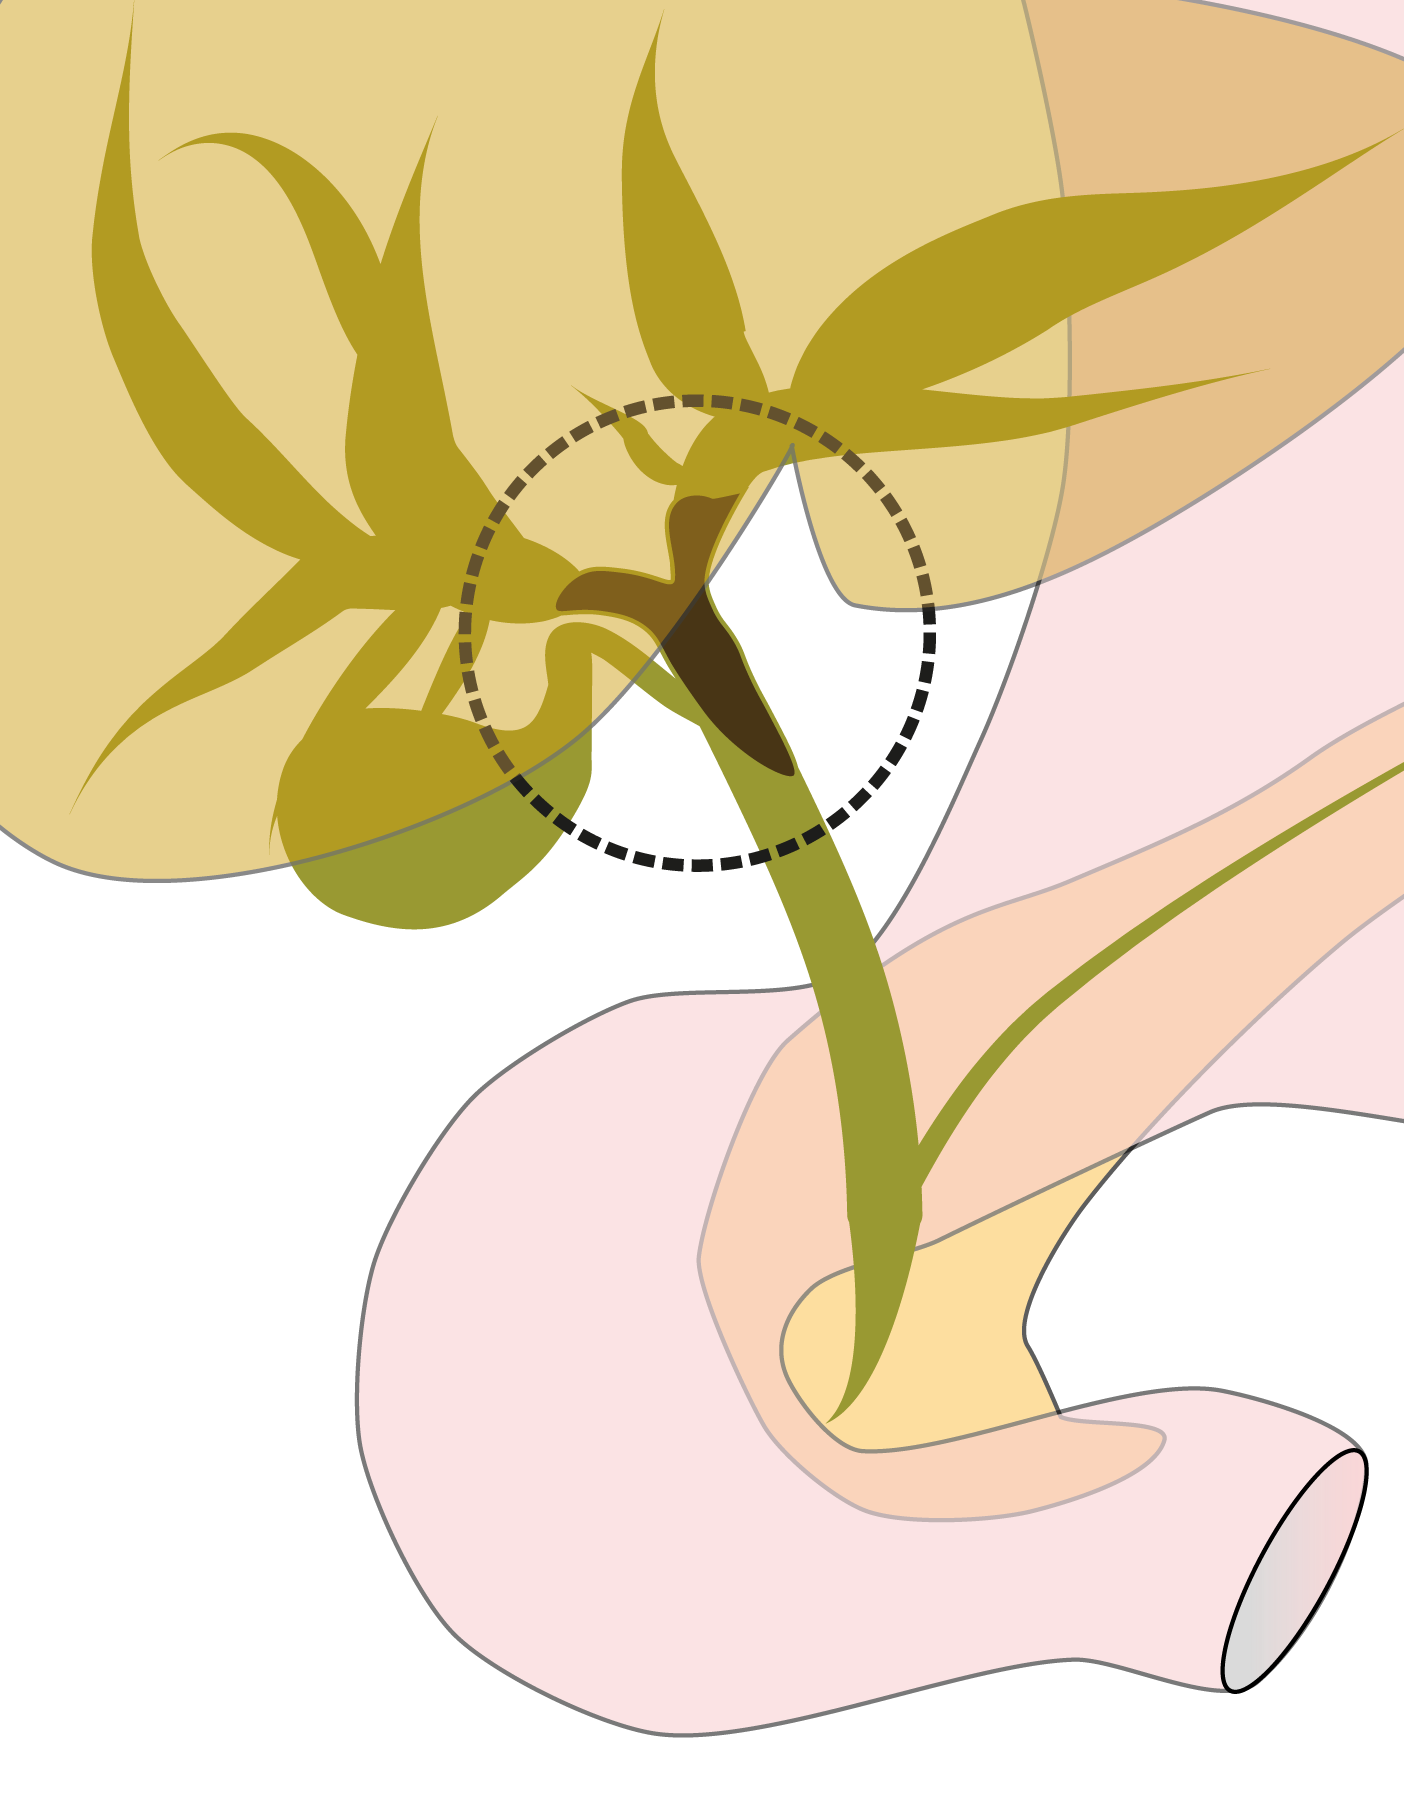
\includegraphics[width=\linewidth]{Figures/PHCC.png}
                \caption{Хіларна холангіокарцинома, або пухлина Клацікіна. Через локалізацію в зоні розвилки жовчних шляхів пухлина перекриває відтік жовчі та призводить до механінчої жовтяниці}
                 \label{fig:phcc}
            \end{marginfigure}
            
            \item рак жовчного міхура
        \end{itemize}
\end{itemize}
	
До вторинних пухлин відносять:
\begin{itemize}
    \item метастази колоректального раку
    \item метастази нейроендокринних пухлин
    \item метастази іншого походження
\end{itemize}

Більшість злоякисних новоутвореннь печінки потребують хірургічного лікування - резекції печінки

\begin{marginfigure}[10pt]%
  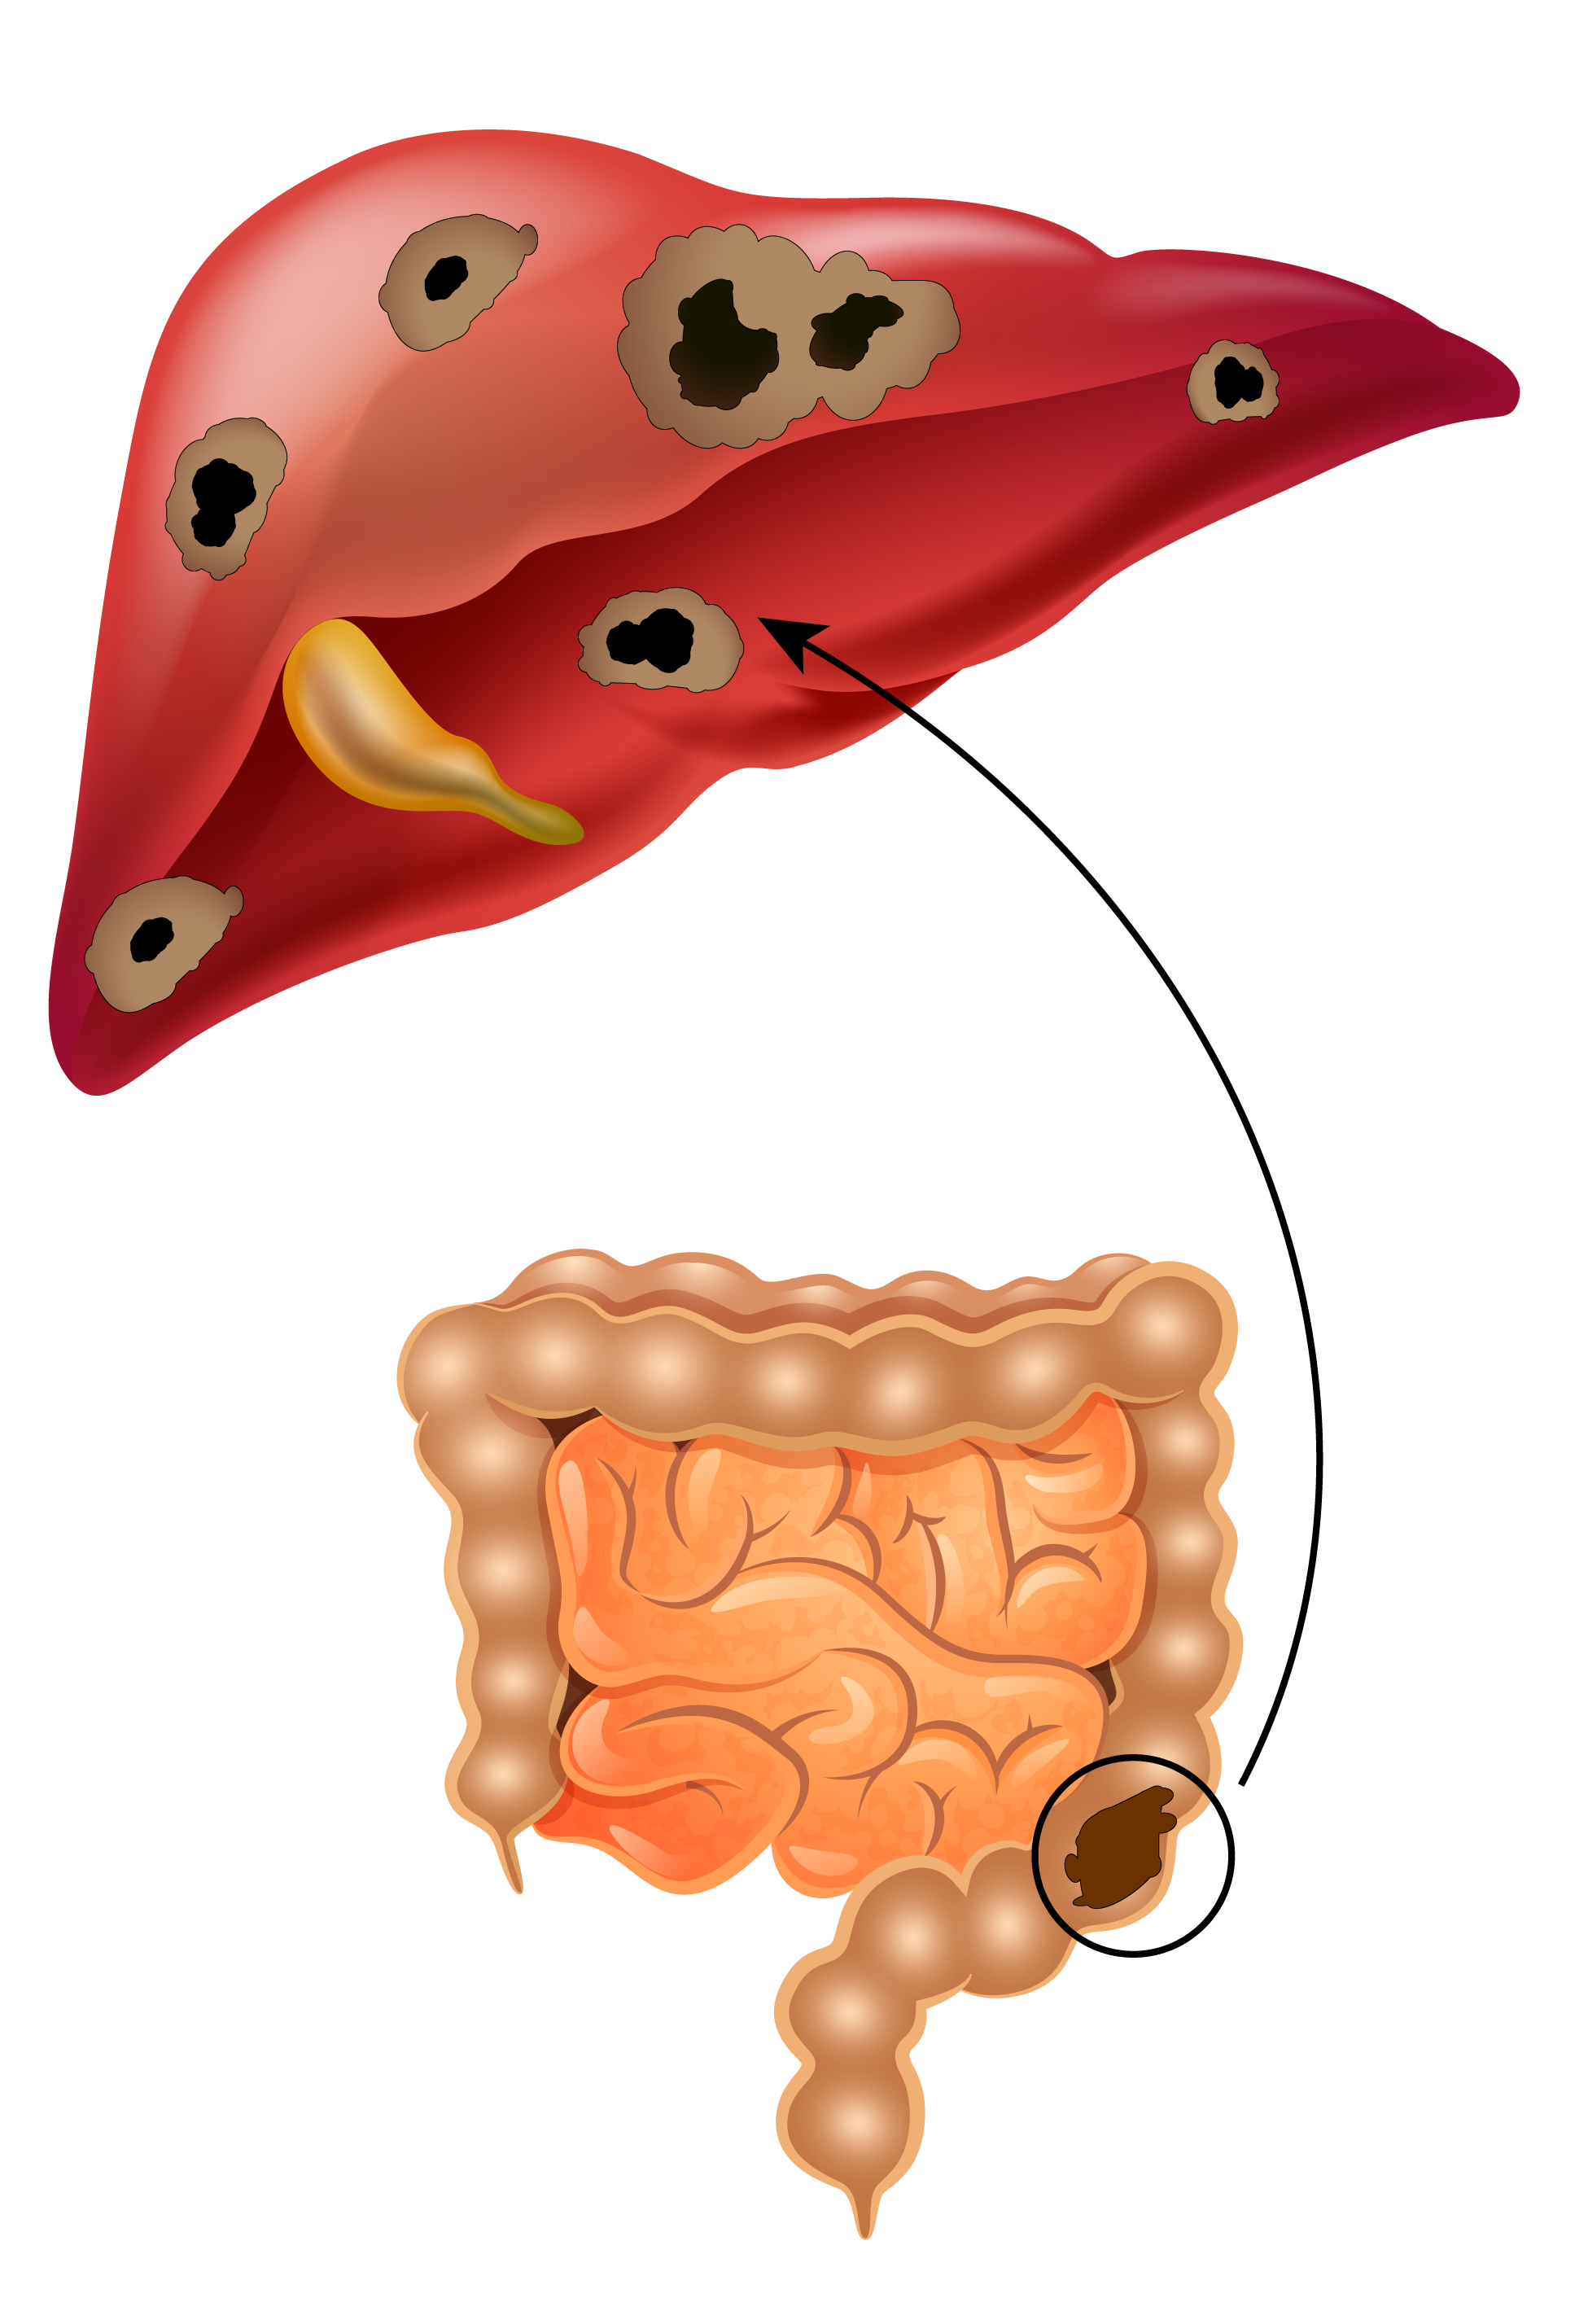
\includegraphics[width=\linewidth]{Figures/CRLM.png}
  \caption{Метастази колоректального раку печінки. Вторинні ураження процес може давати відсіви навіть тоді, коли первинна пухлина видалена}
  \label{fig:crlm}
\end{marginfigure}

\newpage
\section{Які захворювання відносять до доброякісних новоутвореннь печінки?}

До доброякісних новоутвореннь печінки відносять 
\begin{itemize}
    \item гемангіоми
    \item фокальну нодулярну гіперплазію (ФНГ)
    \item аденоми
    \item кісти (прості, ехінококові) та кістозні пухлини печінки (цистаденоми)
\end{itemize}

В більшості випадків при доброякісній патології печінки хірургічне втручання не потрібне. В разі великого симптоматичного ураження або за наявності ризика ускладненнь (розрив, кровотеча, перетворення на злоякісну пухлину) виконують мініінвазивні втручання - пункції кист або абсцесів, лапароскопічні резекції аденом, гемангіом, ФНГ та ін.  


\section{Кому необхідне хірургічне втручання на печінці?}

Хірургічні втручання (\textcolor{red}{резекція}, \textcolor{red}{трансплантація}  або \textcolor{red}{інтервенційне втручання}) на печінці показані пацієнтам, що страждають на вогнищеву або термінальні стадії дифузної патології печінки. 

Рішення про необхідність оперативного втручання після всебічного обстеження приймає виключно мультидисциплінарна коміссія, що обов’язково включає висококваліфікованого фахового спеціаліста - гепатобіліарного хірурга із достатнім клінічним досвідом таких втручаннь.   
\chapter{Резекційна хірургія печінки}

\section{Що таке резекція печінки?}

Резекція печінки -- хірургічна операція по видаленню ураженої частини печінки. 

\begin{figure}
  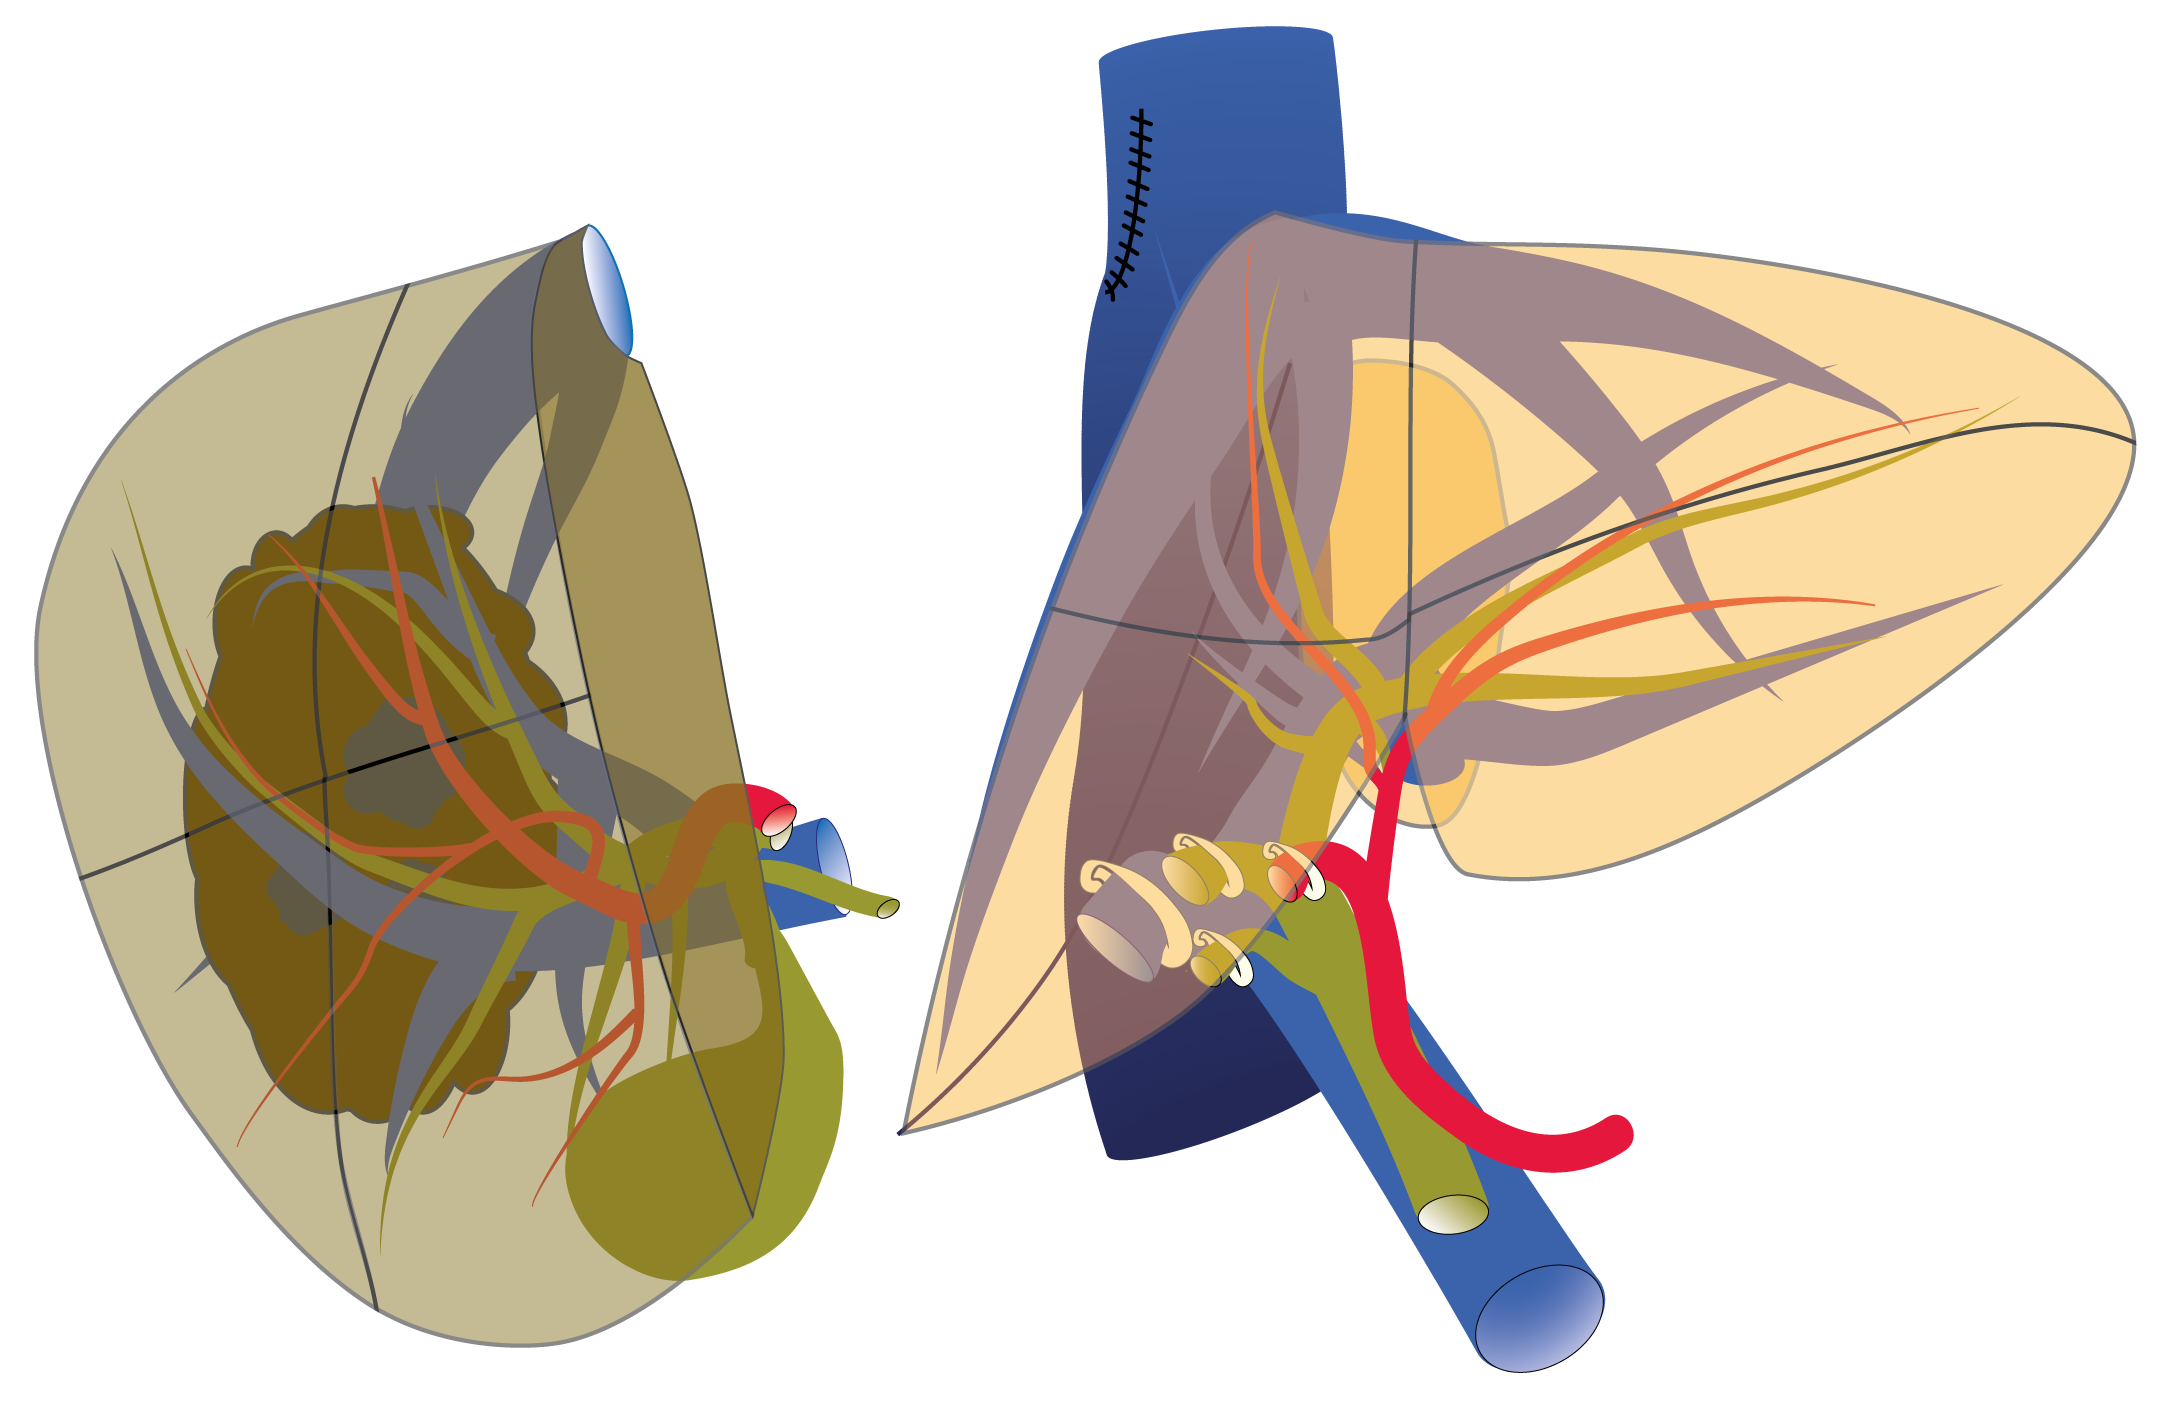
\includegraphics[width=\linewidth]{Figures/Right hepatectomy_Resection.png}
%  \checkparity This is an \pageparity\ page.%
  \caption{Резекція печінки - правобічна гемігепатектомія. Хірург виділяє та перев'язує всі судини, що живлять праву частку печінки, після чого видаляє паренхіму, що містить пухлину. Видалення жовчного міхура є одним з обов'язкових етапів цієї операції.}
  \label{fig:textfig}
  %\zsavepos{pos:textfig}
\end{figure}

Сучасні можливості гепатобіліарної хірургії дозволяють безпечно, із рівнем ускладненнь менше 10\%, виконувати резекцію печінки при ураженні пухлиною близько 70\% тканини печінки. 


\section{При яких захворюваннях необхідна резекція печінки?}

Резекція печінки є методом лікування вогнищевої патології печінки. ЇЇ виконують при злоякісних та доброякісних пухлинах печінки, кистах та хронічних абсцесах печінки.


\section{Які особливості резекцій печінки при онкологічній патології?}

Технічно резекції печінки при онкологічних пухлинах більш обширні та складні, так як можуть потребувати резекції та реконструкції судин чи жовчних протоків, лімфаденектомії та резекції суміжних органів при їх пухлинній інвазії. 

\begin{marginfigure}%
  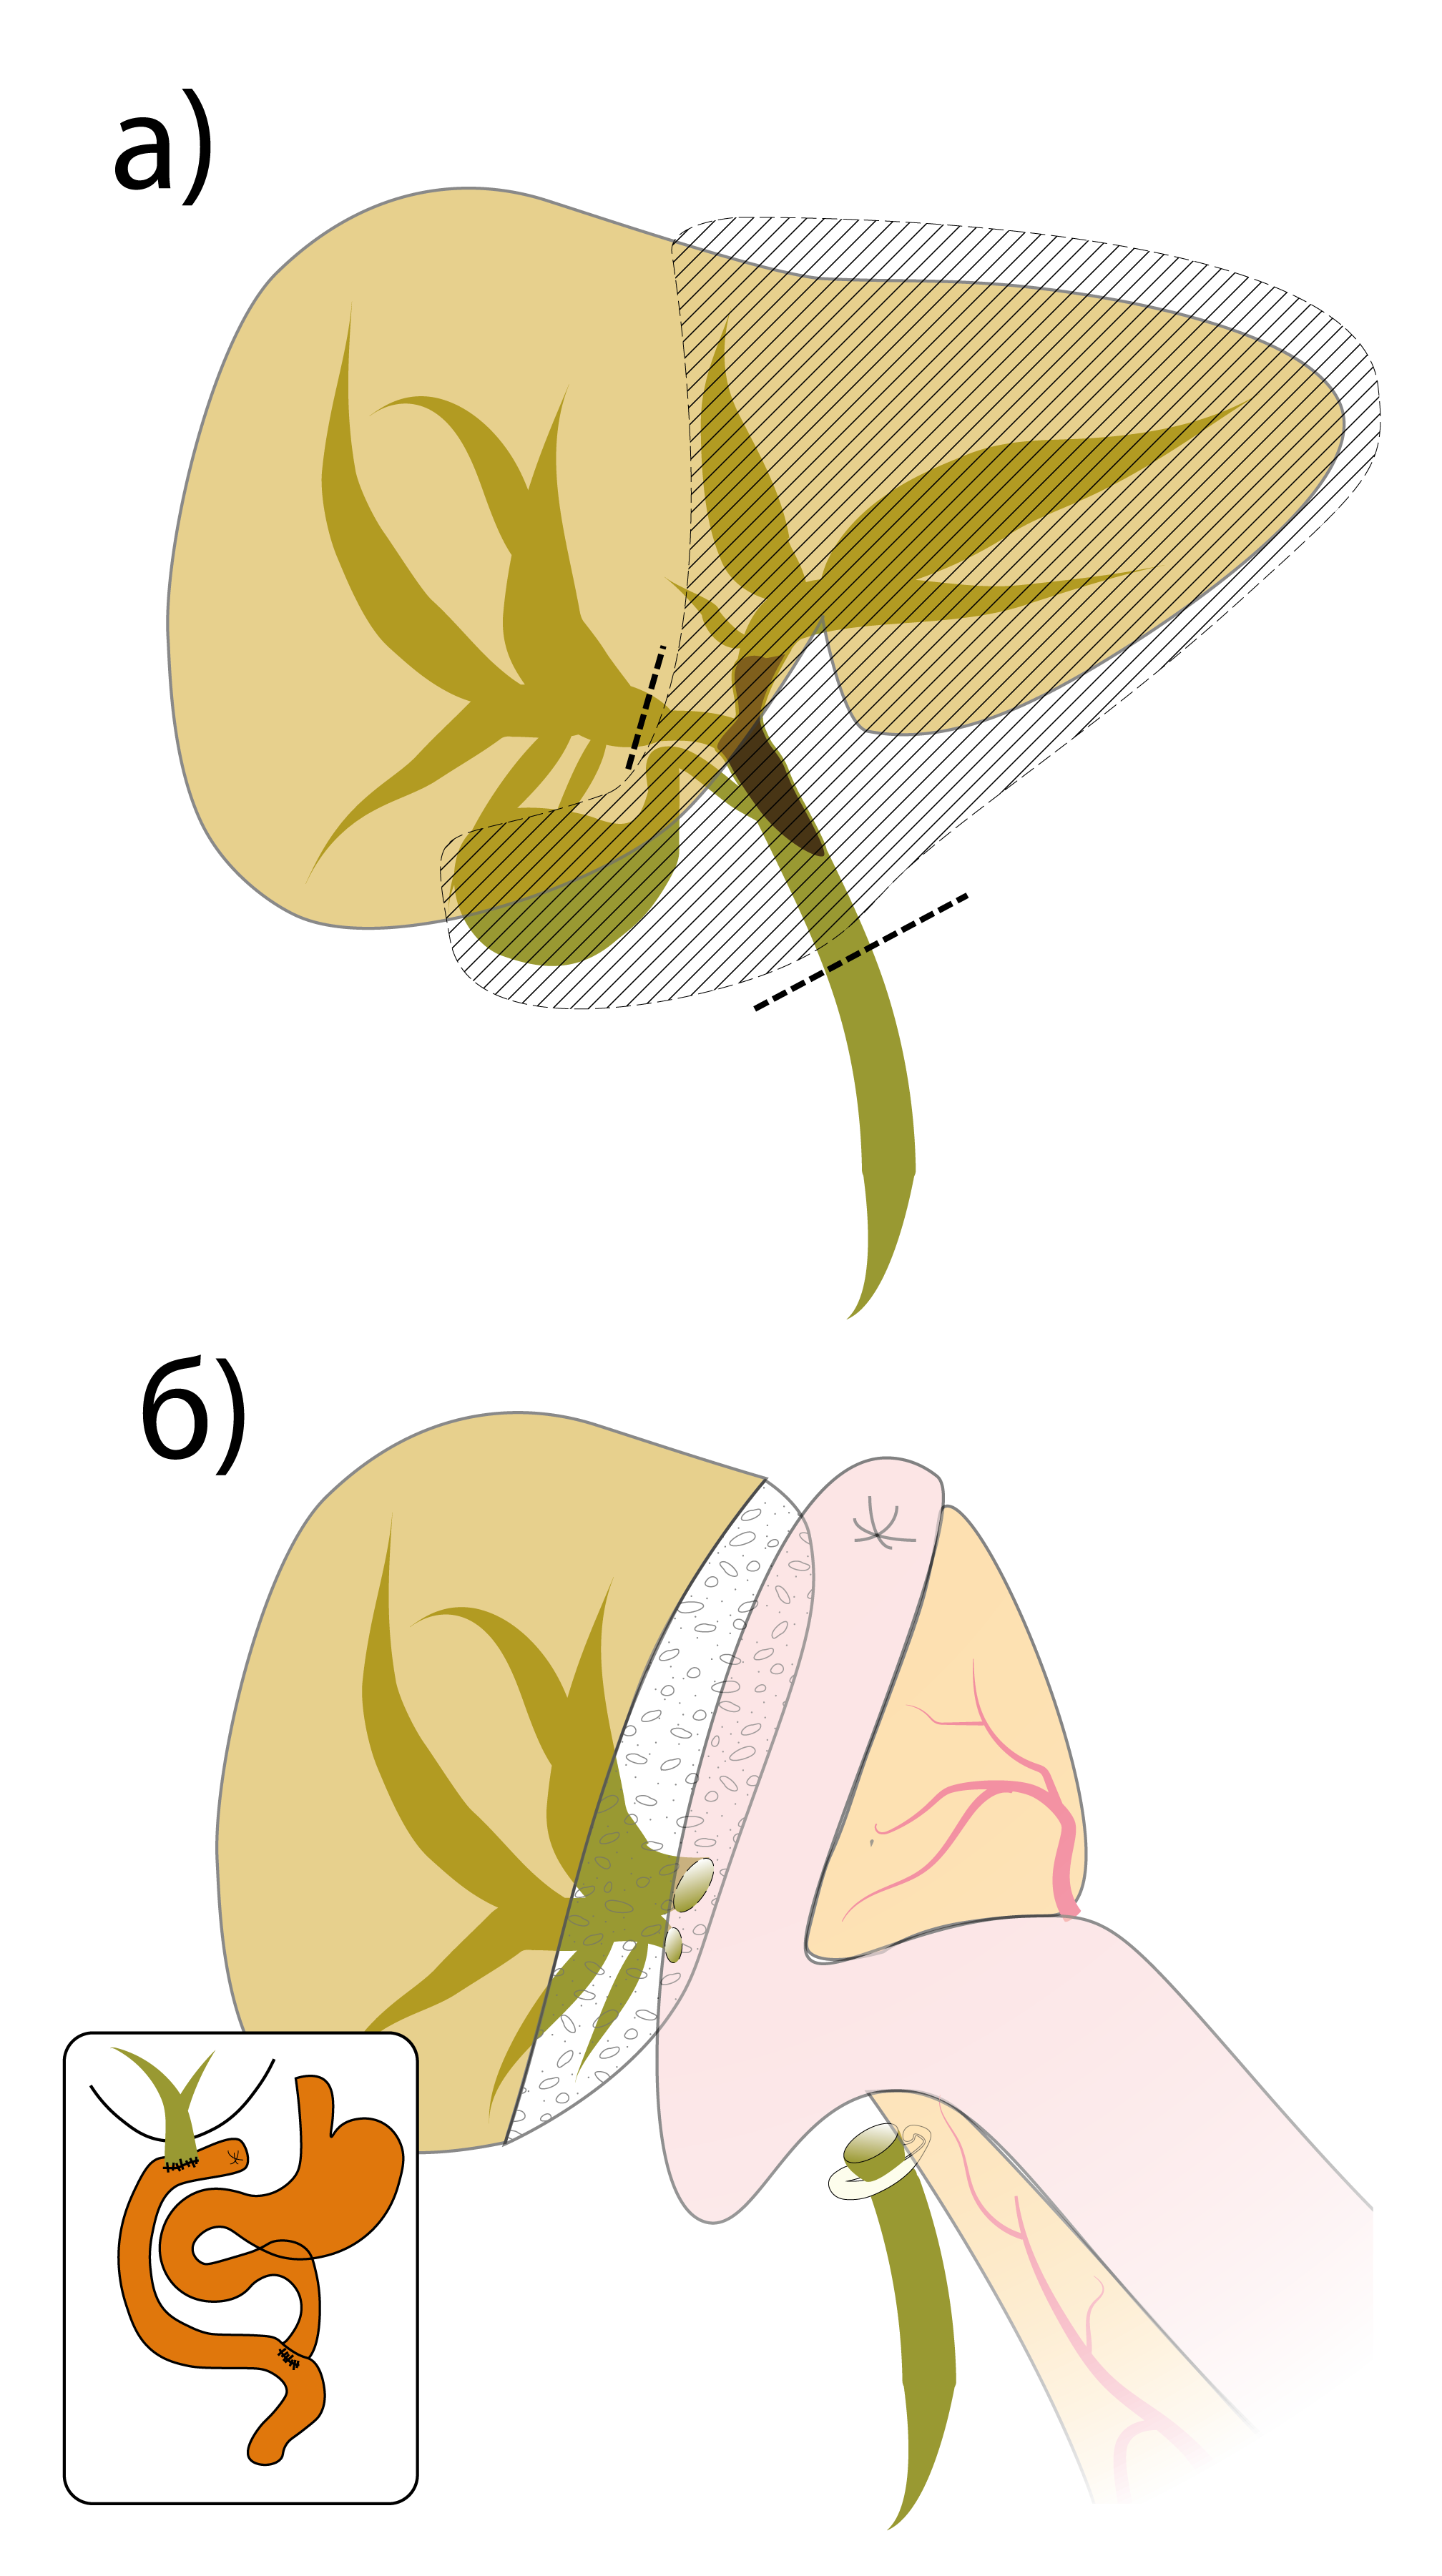
\includegraphics[width=\linewidth]{Figures/Bile duct resection.png}
  \caption{Резекція та реконструкція жовчних шляхів при пухлинному ураженні. 
  а) планований до видалення об'єм печінки (помічено сірою штриховкою), який включає печінку з пухлиною та уражені нею жовчні шляхи; б) реконструкція -- вільний від пухлини край жовчних шляхів зшивається із петлею тонкої кишки для відводу туди жовчі}
  \label{fig:crlm}
\end{marginfigure}

\begin{tcolorbox}[width=\textwidth,colback=red!5!white,colframe=red!75!black]    
Онкологічні захворювання -- складна проблема, яка потребує мультидисциплінарного підходу. Резекція печінки є формою локального контролю пухлини, що  застосовується в комбінації із іншими способами лікування. 
\end{tcolorbox}    


Необхідність проведення додаткового лікування перед чи після резекції печінки (наприклад адьювантної хіміотерапії) гепатобіліарний хіург визначає у складі  мультидисциплінарної комісії.



\section{Які є різновиди резекцій печінки?}

\begin{enumerate}
    \item За об’ємом тканини, що видаляється резекції печінки поділяють на звичайні та обширні, коли видаляється чотири або більше сегментів печінки
    \item За підходом до видалення резекції печінки діляться на анатомічні резекції, коли новоутворення видяляється разом із сегментом, в якому знаходиться (див. сегменти печінки) та субсегментарні енуклеорезекції, коли новоутворення видяляється разом із невеликим шаром оточуючої паренхіми в межах здорової тканини
    \item За хірургічниим доступом резекції печінки діляться на відкриті (або традиційні) та лапароскопічні 
\end{enumerate}

\begin{figure}
  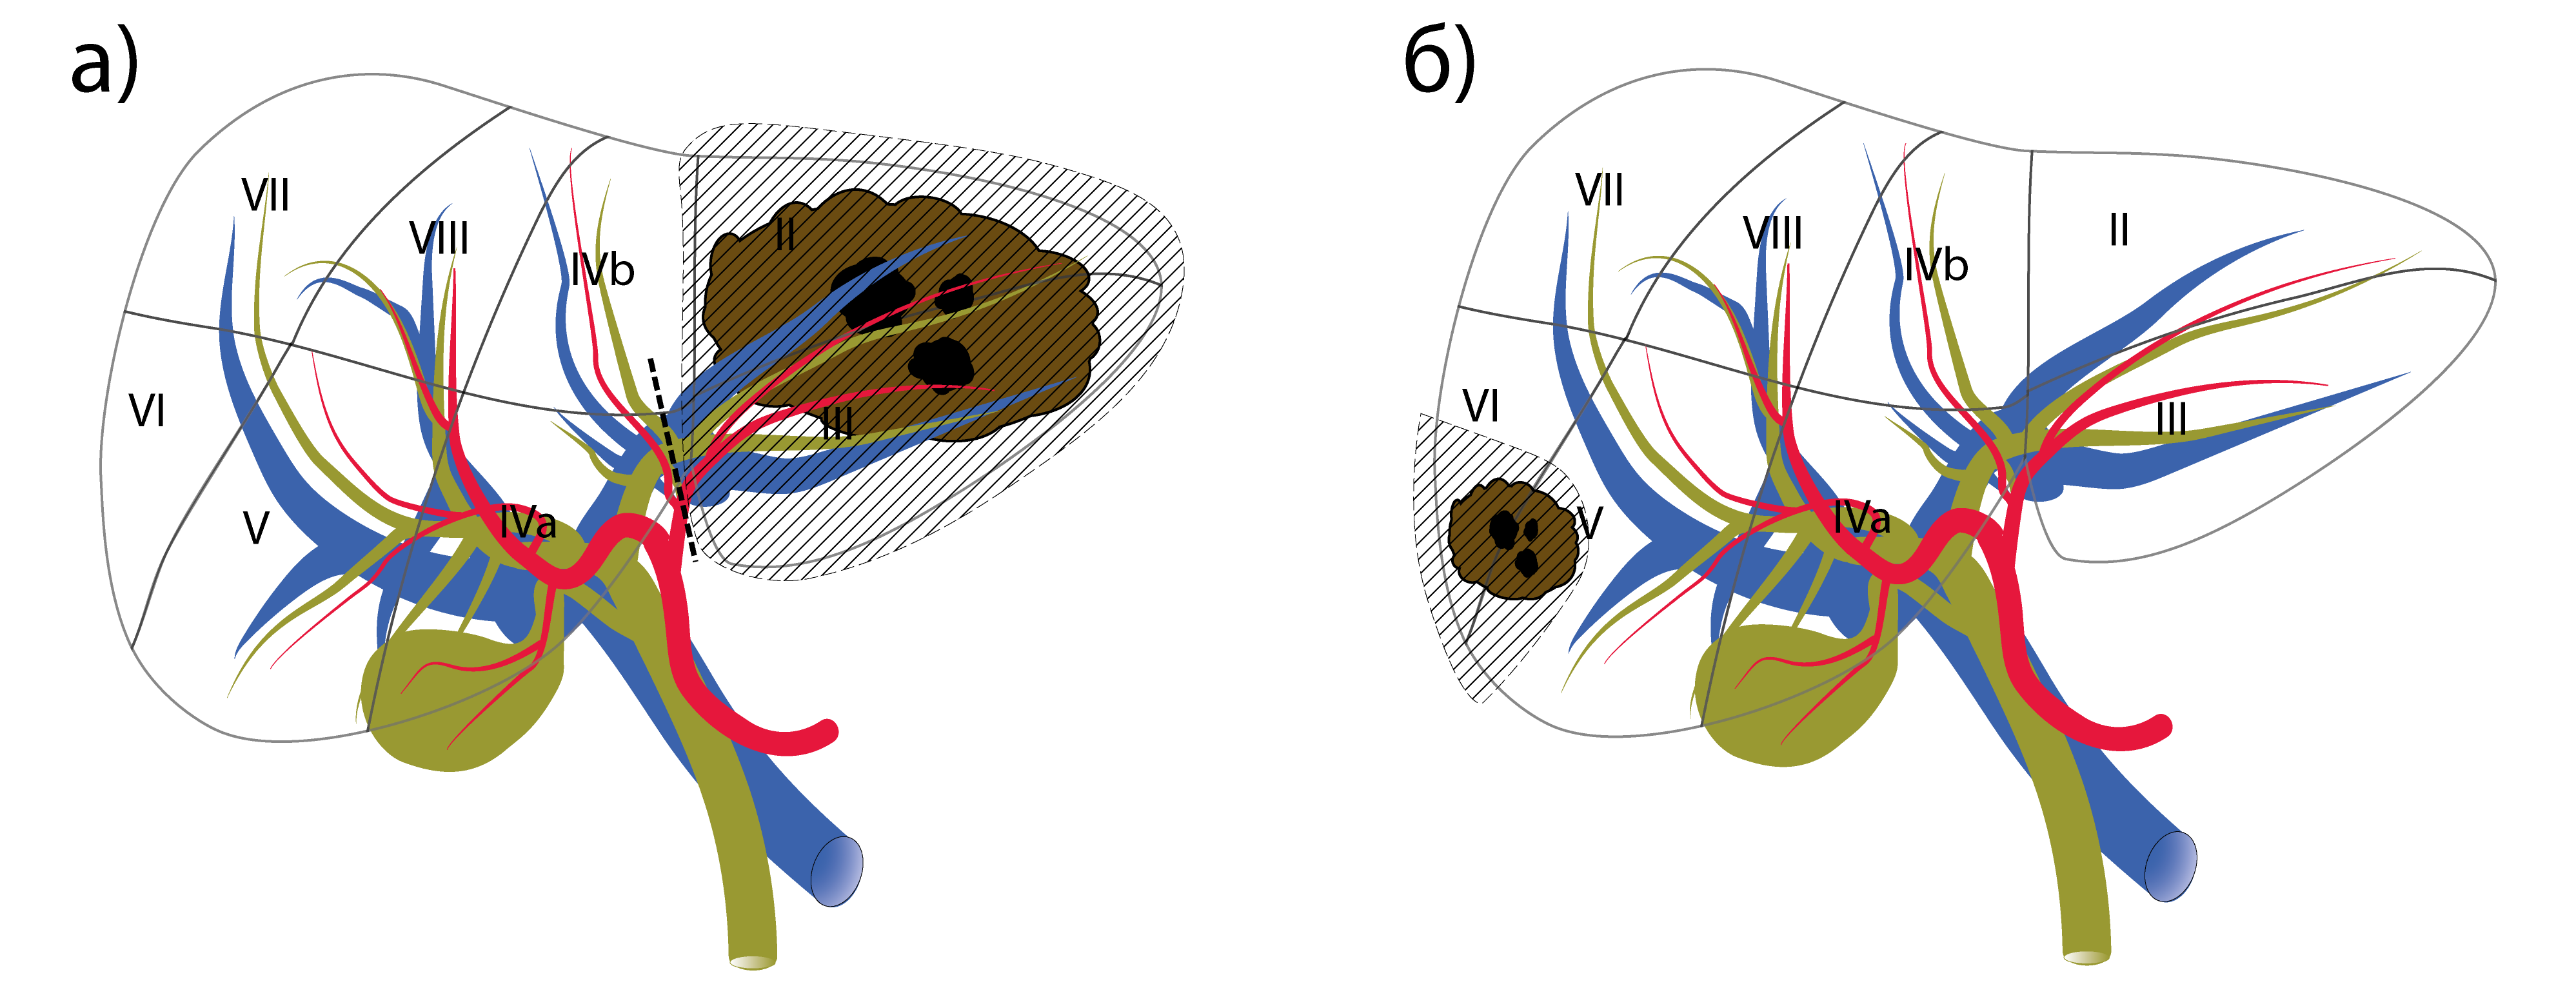
\includegraphics[width=\linewidth]{Figures/Anatomical vs marginal_Horizontal.png}
%  \checkparity This is an \pageparity\ page.%
  \caption{Прилади анатомічної (а) та крайової (б) резекції. При анатомічній резекції спочатку виділяють та пересікають судини, що живлять відповідні сегменти, а потім по лінії знекровлення проводять відсіченя паренїми. При крайовій енуклеорезекції лінія транссекції намічається з відступом 1-2 см від краю пухлини}
  \label{fig:textfig}
  %\zsavepos{pos:textfig}
\end{figure}

\newpage
\section{Як виконується відкрита (традиційна) резекція печінки?}

При відкритій або традиційній резекції печінки доступ до органа відбувається шляхом лапаротомії - великого розрізу на передній черевній стінці із наступним широким розведенням країв рани, що забезпечує хірургу максимально широке поле дії для операції. Такий доступ дозволяє виконувати надскладні операції при вростанні пухлин в великі судини печінки або жовчні протоки. 

\begin{marginfigure}[10pt]%
  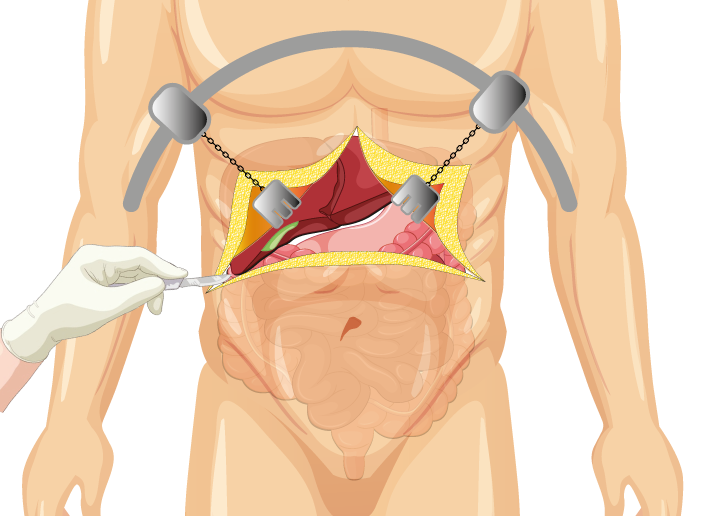
\includegraphics[width=\linewidth]{Figures/LapVsOpen_Open surgery.png}
  \caption{Схема хірургічного доступу при відкритій резекції печінки. Хірург оперує через широкий Т-подібний доступ типу "мерседес". Края рани розтягуються спеціальними ретракторами на лебідках.}
  \label{fig:crlm}
\end{marginfigure}

\section{Що таке лапароскопія?}

Лапароскопія  - це високотехнологічна хірургічна методика, яка дозволяє отримати зображення внутрішніх органів та проводити маніпуляції на них без розрізу передньої черевної стінки за рахунок спеціального ендовідеохірургічного обладнання.

Лапароскопічні операції - безпечний метод лікування, що застосовується у всіх сучасних клініках. На теперішньому етапі розвитку хірургії в лапароскопічному варіанті доступна абсолютна більшість хірургічних операцій. 

Через свої переваги для пацієнтів при певних видах операцій (наприклад холецистектомія - видалення жовчного міхура) лапароскопія стала золотим стандартом лікування, залишивши відкритий доступ лише для виключних випадків. 

Під час проведення лапароскопічної операції хірург маніпулює в черевній порожнині спеціальними довгими інструментами під контролем зображення з відеокамери, яке виводиться на високоякісний медичний монітор.\sidenote[][-120pt]{Зображення органів черевної порожнини потрапляє в відеокамеру через лапароскоп - хірургічний інструмент, який має форму довгої та тонкої металевої трубки, в середині якої знаходяться оптичні лінзи та оптоволокно. Технічно лапароскоп є медичним аналогом об’єктиву звичайної камери.

Лапароскоп та хірургічні інструменти в живіт пацієнта вводять через спеціальні порти - пристрої  у вигляді короткої трубки з клапаном, що дозволяють утримувати в  черевній порожнині вуглекислий газ, що створює робочий простір для хірурга. 
}


\begin{marginfigure}[40pt]%
  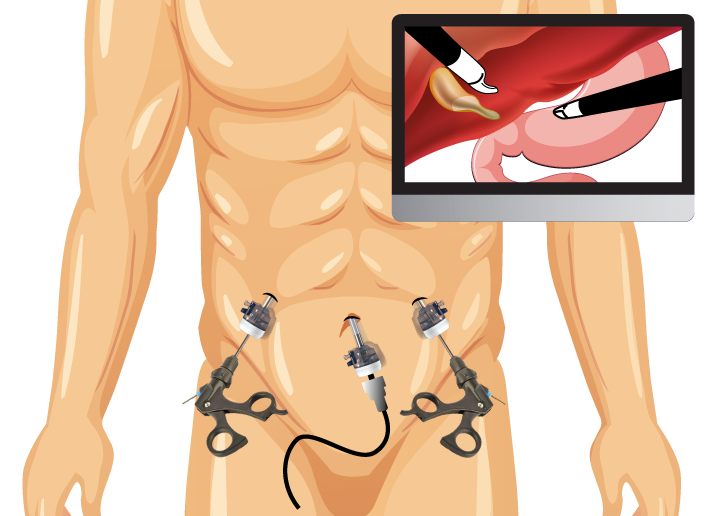
\includegraphics[width=\linewidth]{Figures/LapVsOpen_Laparoscopic surgery.png}
  \caption{Схема хірургічного доступу при лапароскопічній резекції печінки. Хірург оперує через маленькі розрізи спеціальними інструментами під контролем зображення, отриманого з відеокамери на моніторі}
  \label{fig:crlm}
\end{marginfigure}




\section{Що таке лапароскопічна резекція печінки?}

Лапароскопічна резекція печінки - це високотехнологічна хірургічна операція по видаленню частини печінки, яка виконується лапароскопічним шляхом, через маленькі проколи в черевній стінці під контролем відеокамери. 

\begin{tcolorbox}[width=\textwidth,colback=yellow!5!white,colframe=yellow!75!black]    
За об’ємом видаляємої паренхіми лапароскопічні резекції аналогічні відкритим, тобто для мініінвазивного підходу доступні всі ті самі об’єми операцій, включаючи обширні резекції, що і для традиційного.
\end{tcolorbox}    

Єдиним умовним обмеженням є вростання пухлини в магістральні судини або жовчні протоки.

Видалена частина печінки при лапароскопічних резекціях видаляється через невеликий атравматичний розріз, довжиною 5 см внизу живота.


\section{Які переваги надає лапароскопічна резекція печінки?}


Лапароскопічна резекція в порівнянні із відкритими операціями дозволяє хворому отримати:
\begin{itemize}
    \item аналогічний відкритим операціям онкологічний ефект при злоякісних захворюваннях
    \item меншу кількість післяопераційних ускладнень
    \item менш виражений больовий синдром та післяопераційний стрес
    \item пришвидшену реабілітацію та більш повне функціональне відновлення
    \item відсутність травматизації передньої черевної стінки та збереження функції м’язів преса
    \item кращий косметичний ефект
\end{itemize}
	

\section{Кому показана відкрита, а кому лапароскопічна резекція печінки?}

\begin{tcolorbox}[width=\textwidth,colback=green!5!white,colframe=green!75!black]    
В більшості випадків, при неускладнених формах пухлин будь-якого походження можливо виконати резекцію печінки в лапароскопічному варіанті, що надає пацієнту покращений профіль безпеки та адекватну онкологічну ефективність.
\end{tcolorbox}    

У випадку проростання пухлин в магістральні судини або жовчні протоки методом вибору залишається відкрита резекція печінки.

\section{Хто обирає об'єм резекції та хірургічний доступ?}
В процесі обстеження пацієнта хірург визначає покази до хірургічного лікування та його об'єм. Після отримання результатів обстеження хірург обговорює їх з пацієнтом, знайомить його з можливим планом лікування. За відсутності протипоказів під час цього обговорення пацієнт може віддати перевагу відкритому чи лапароскопічному варіанту виконання операції.
  
\chapter{Інтервенційні втручання}


\section{Які є види інтервенційних втручаннь на печінці?}
Інтервенційні втручання - група мініінвазивних методик, що використовують в якості допоміжного або самостійного метода локорегіонального лікування патології печінки.  Як правило такі втручання виконують під ангіографічним, рентген, УЗД або КТ контролем.

До них відносять:
\begin{itemize}
    \item Ендоваскулярні методики
    \begin{itemize}
        \item трансартеріальна хемоемболізація пухлин - локальна хіміотерапія, коли медиамент доставляється безпосередньо до пухлини через печінкову артерію)
        
        \begin{marginfigure}%
            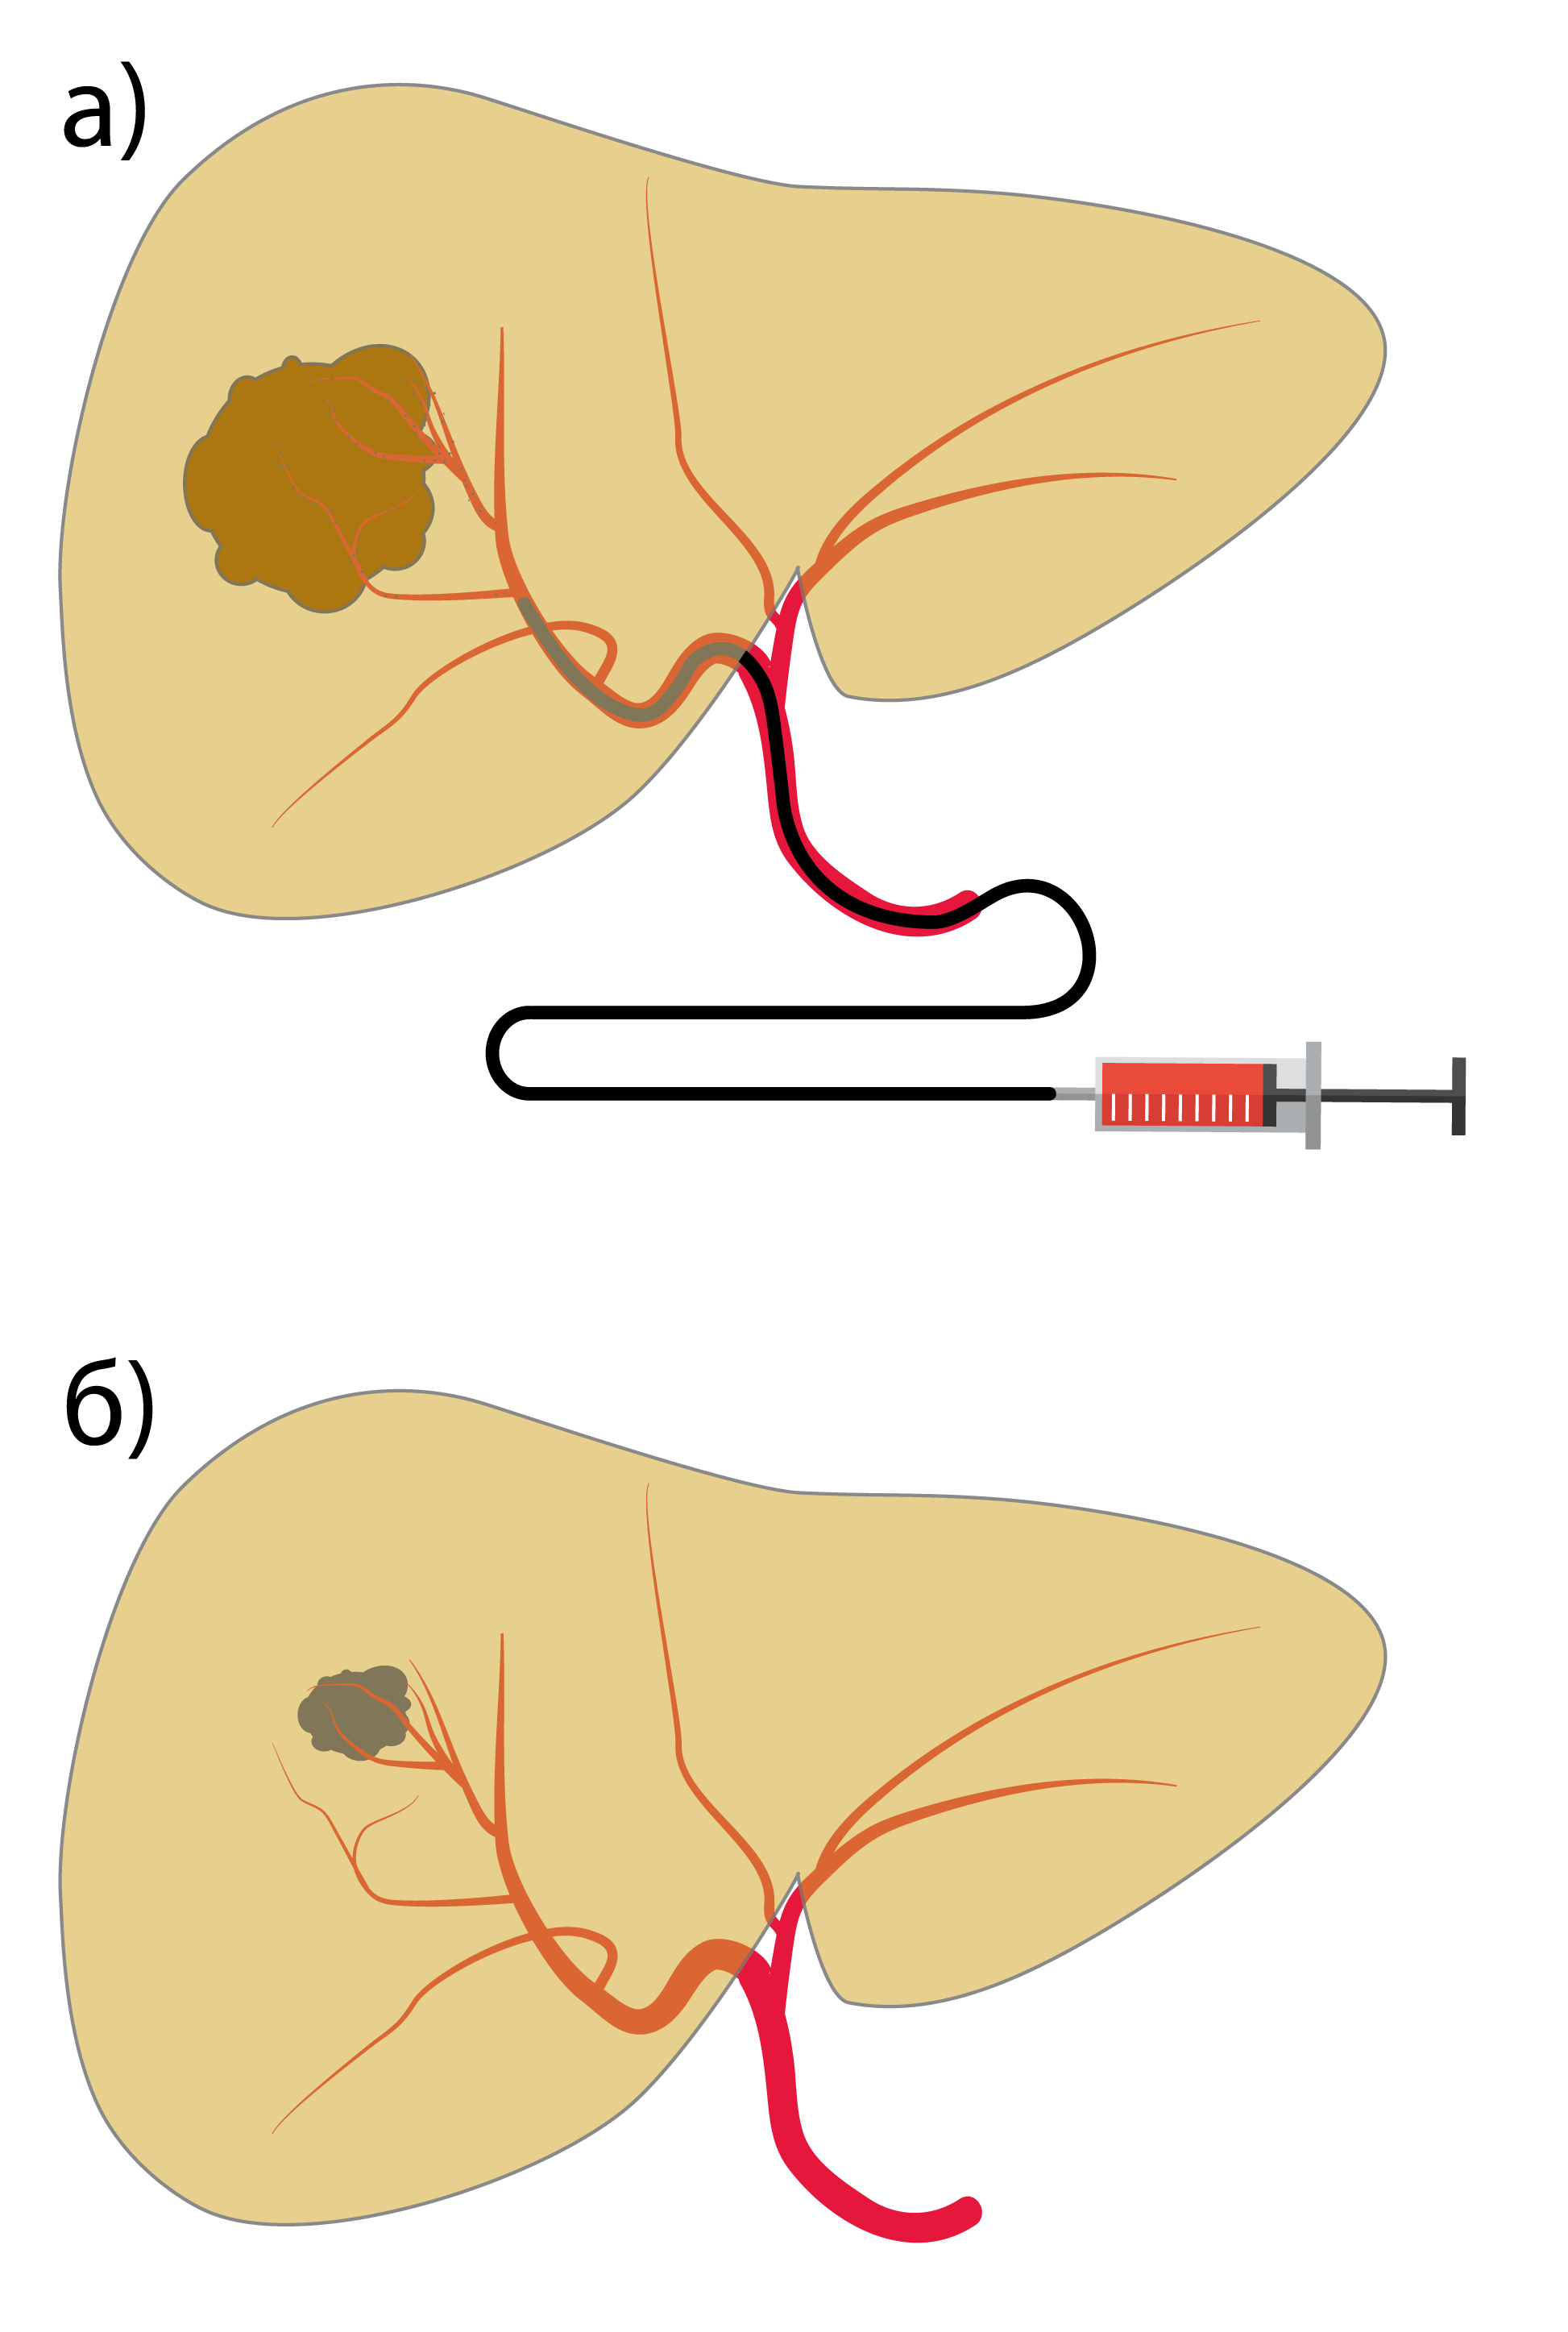
\includegraphics[width=\linewidth]{Figures/TACE_Vertical.png}
            \caption{Трансартеріальна хемоемболізація печінкової артерії (TACE) а) хіміопрепарат вводиться безпосередньо в пухлину через гілку печінкової артерії б) зменьшення та некроз пухлини через 1 місяць }
            \label{fig:goalbladder}
        \end{marginfigure}
        
        \item емболізація ворітної вени - ендоваскулярна процедура перекриття кровотоку по ворітній вені до пухлини. Застосовується в якості передопераційної підготовки для збільшення печінкового залишку перед виконанням резекції печінки
        
        \begin{marginfigure}%
            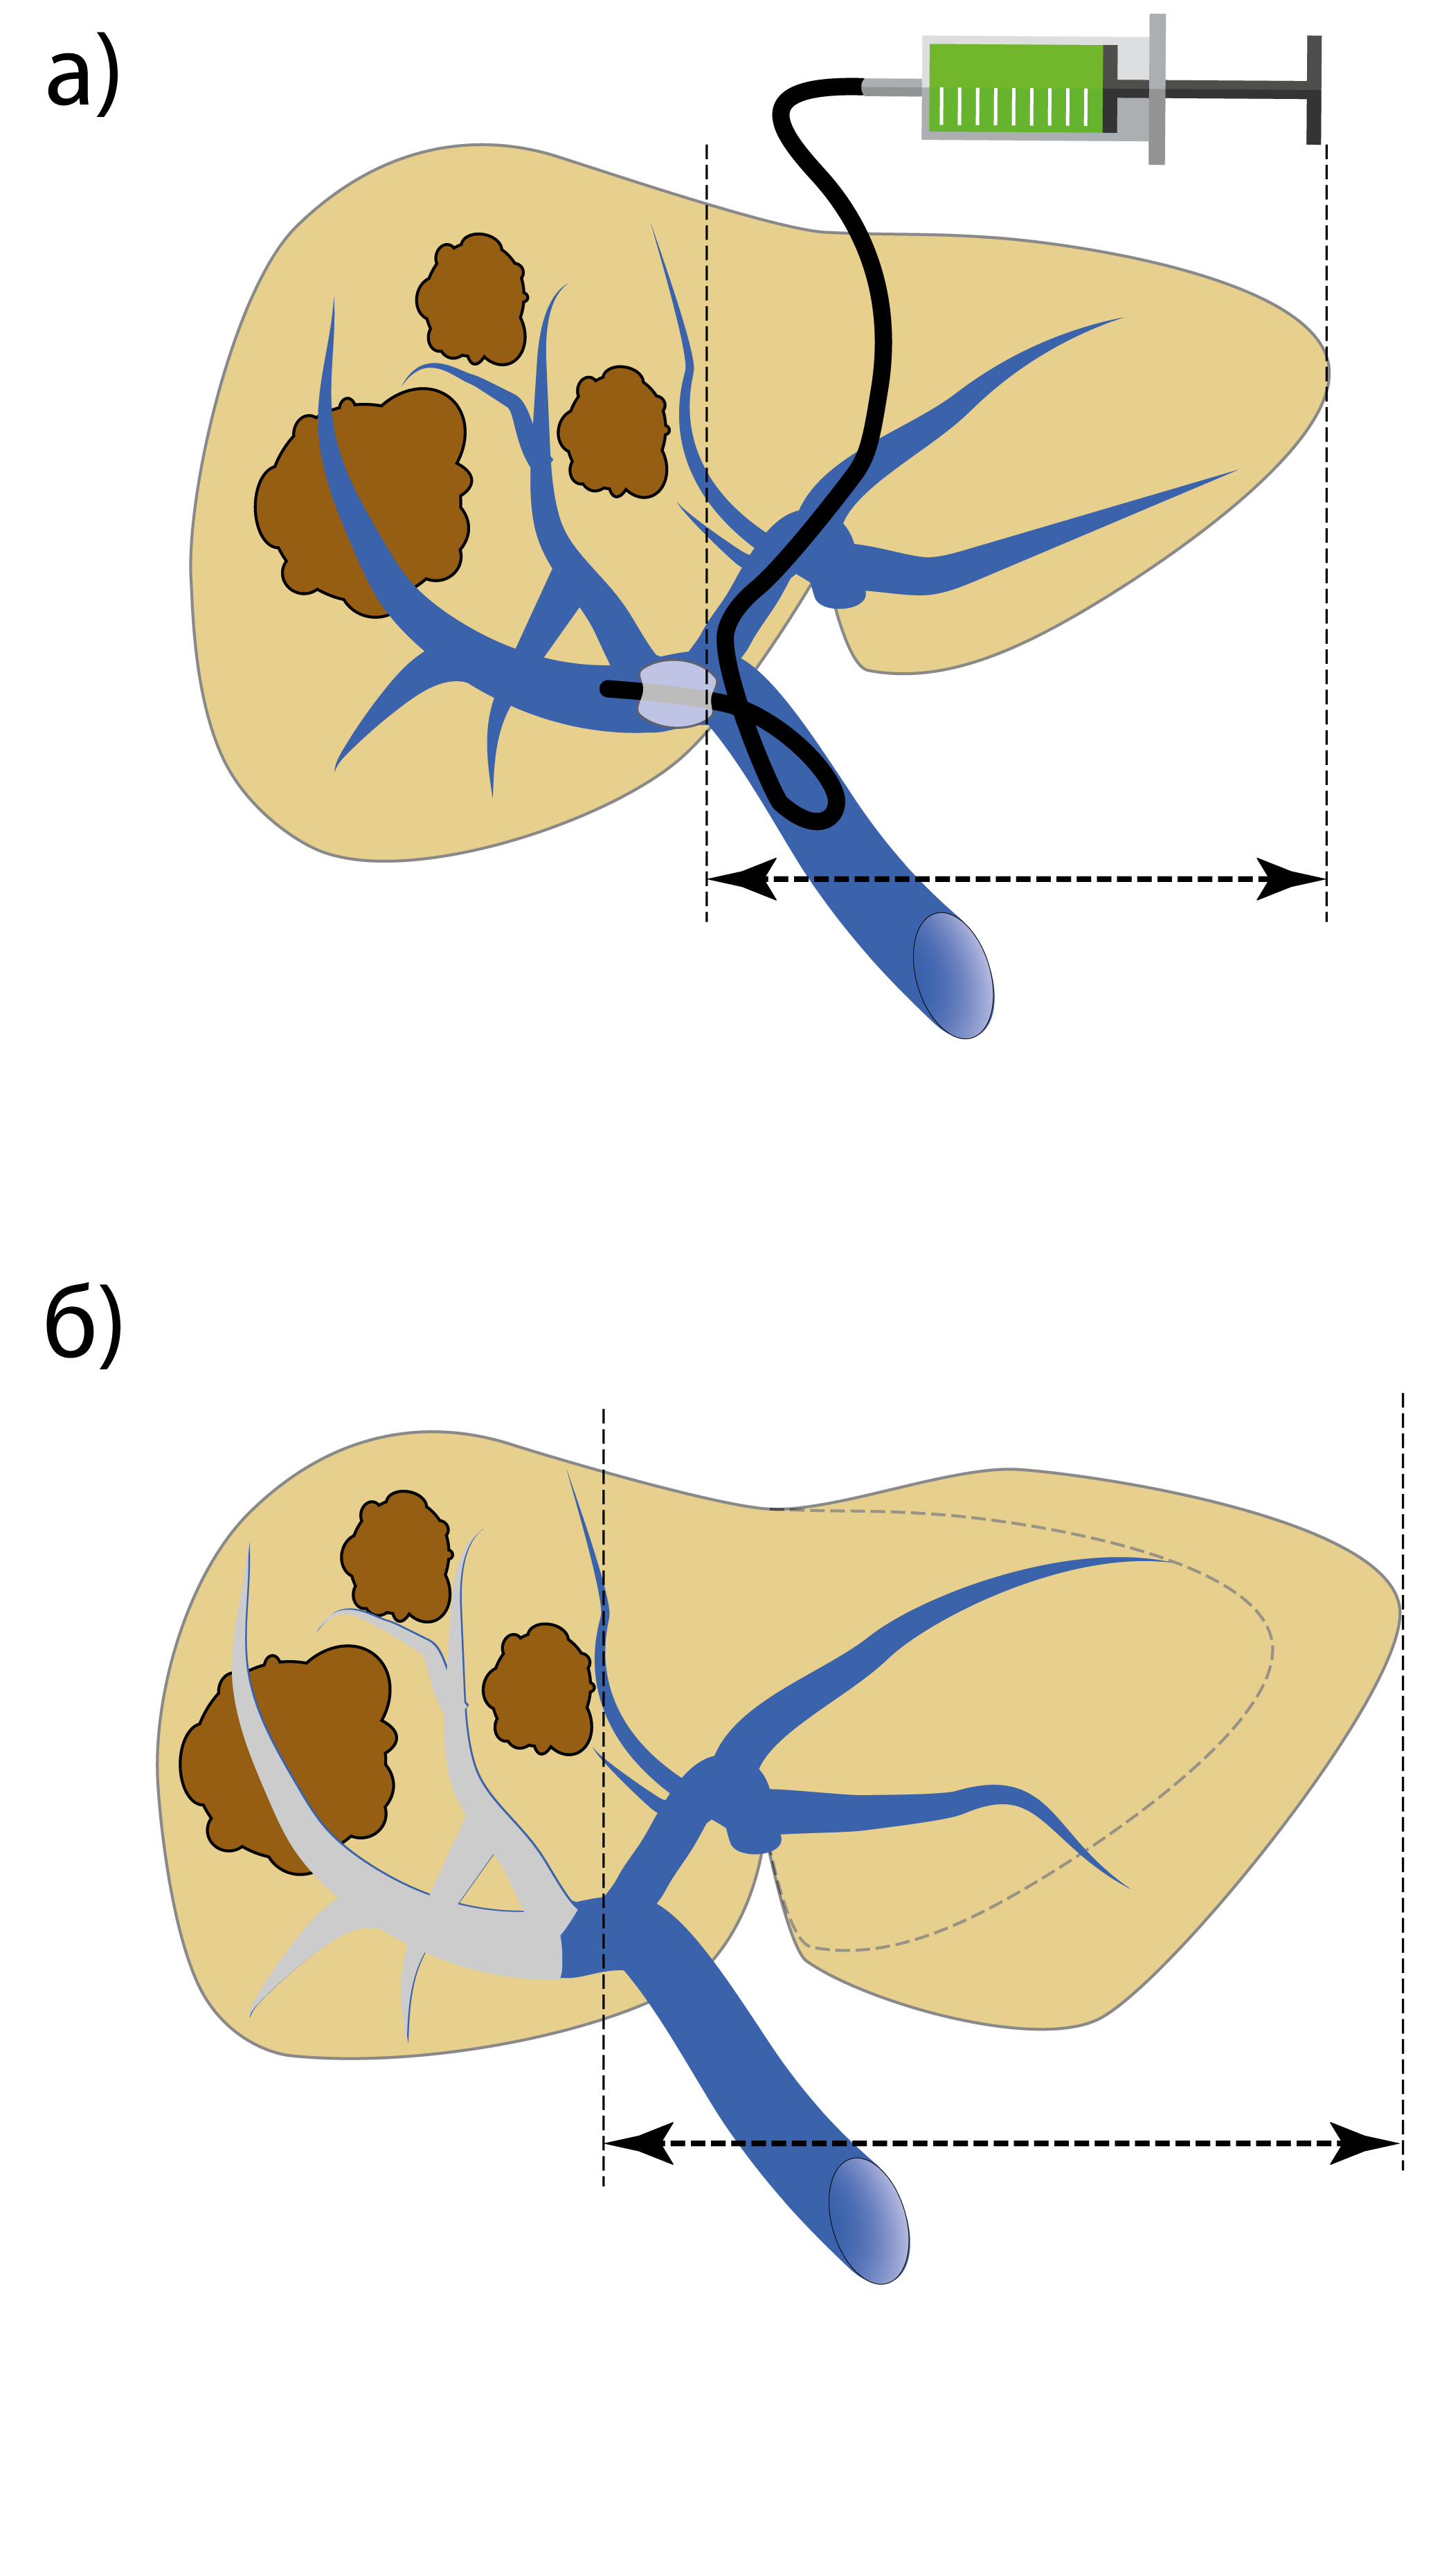
\includegraphics[width=\linewidth]{Figures/PVE_Vertical.png}
            \caption{Емболізація ворітної вени. а) мікроемболи вводяться в просвіт ворітної вени для перекриття кровотоку на уражену частину печінки б) збільшення потенційного печінкового залишку через 3-4 тижні }
            \label{fig:goalbladder}
        \end{marginfigure}
        
    \end{itemize}
    \item УЗ-контрольовані втручання
    \begin{itemize}
        \item абляція пухлин новоутвореннь печінки - знищення пухлини за допомогою локальної дії змінного електричного високочастотного струму, радіохвиль чи етанолу. Виконується під УЗ- або КТ- контролем 
        \begin{marginfigure}%
            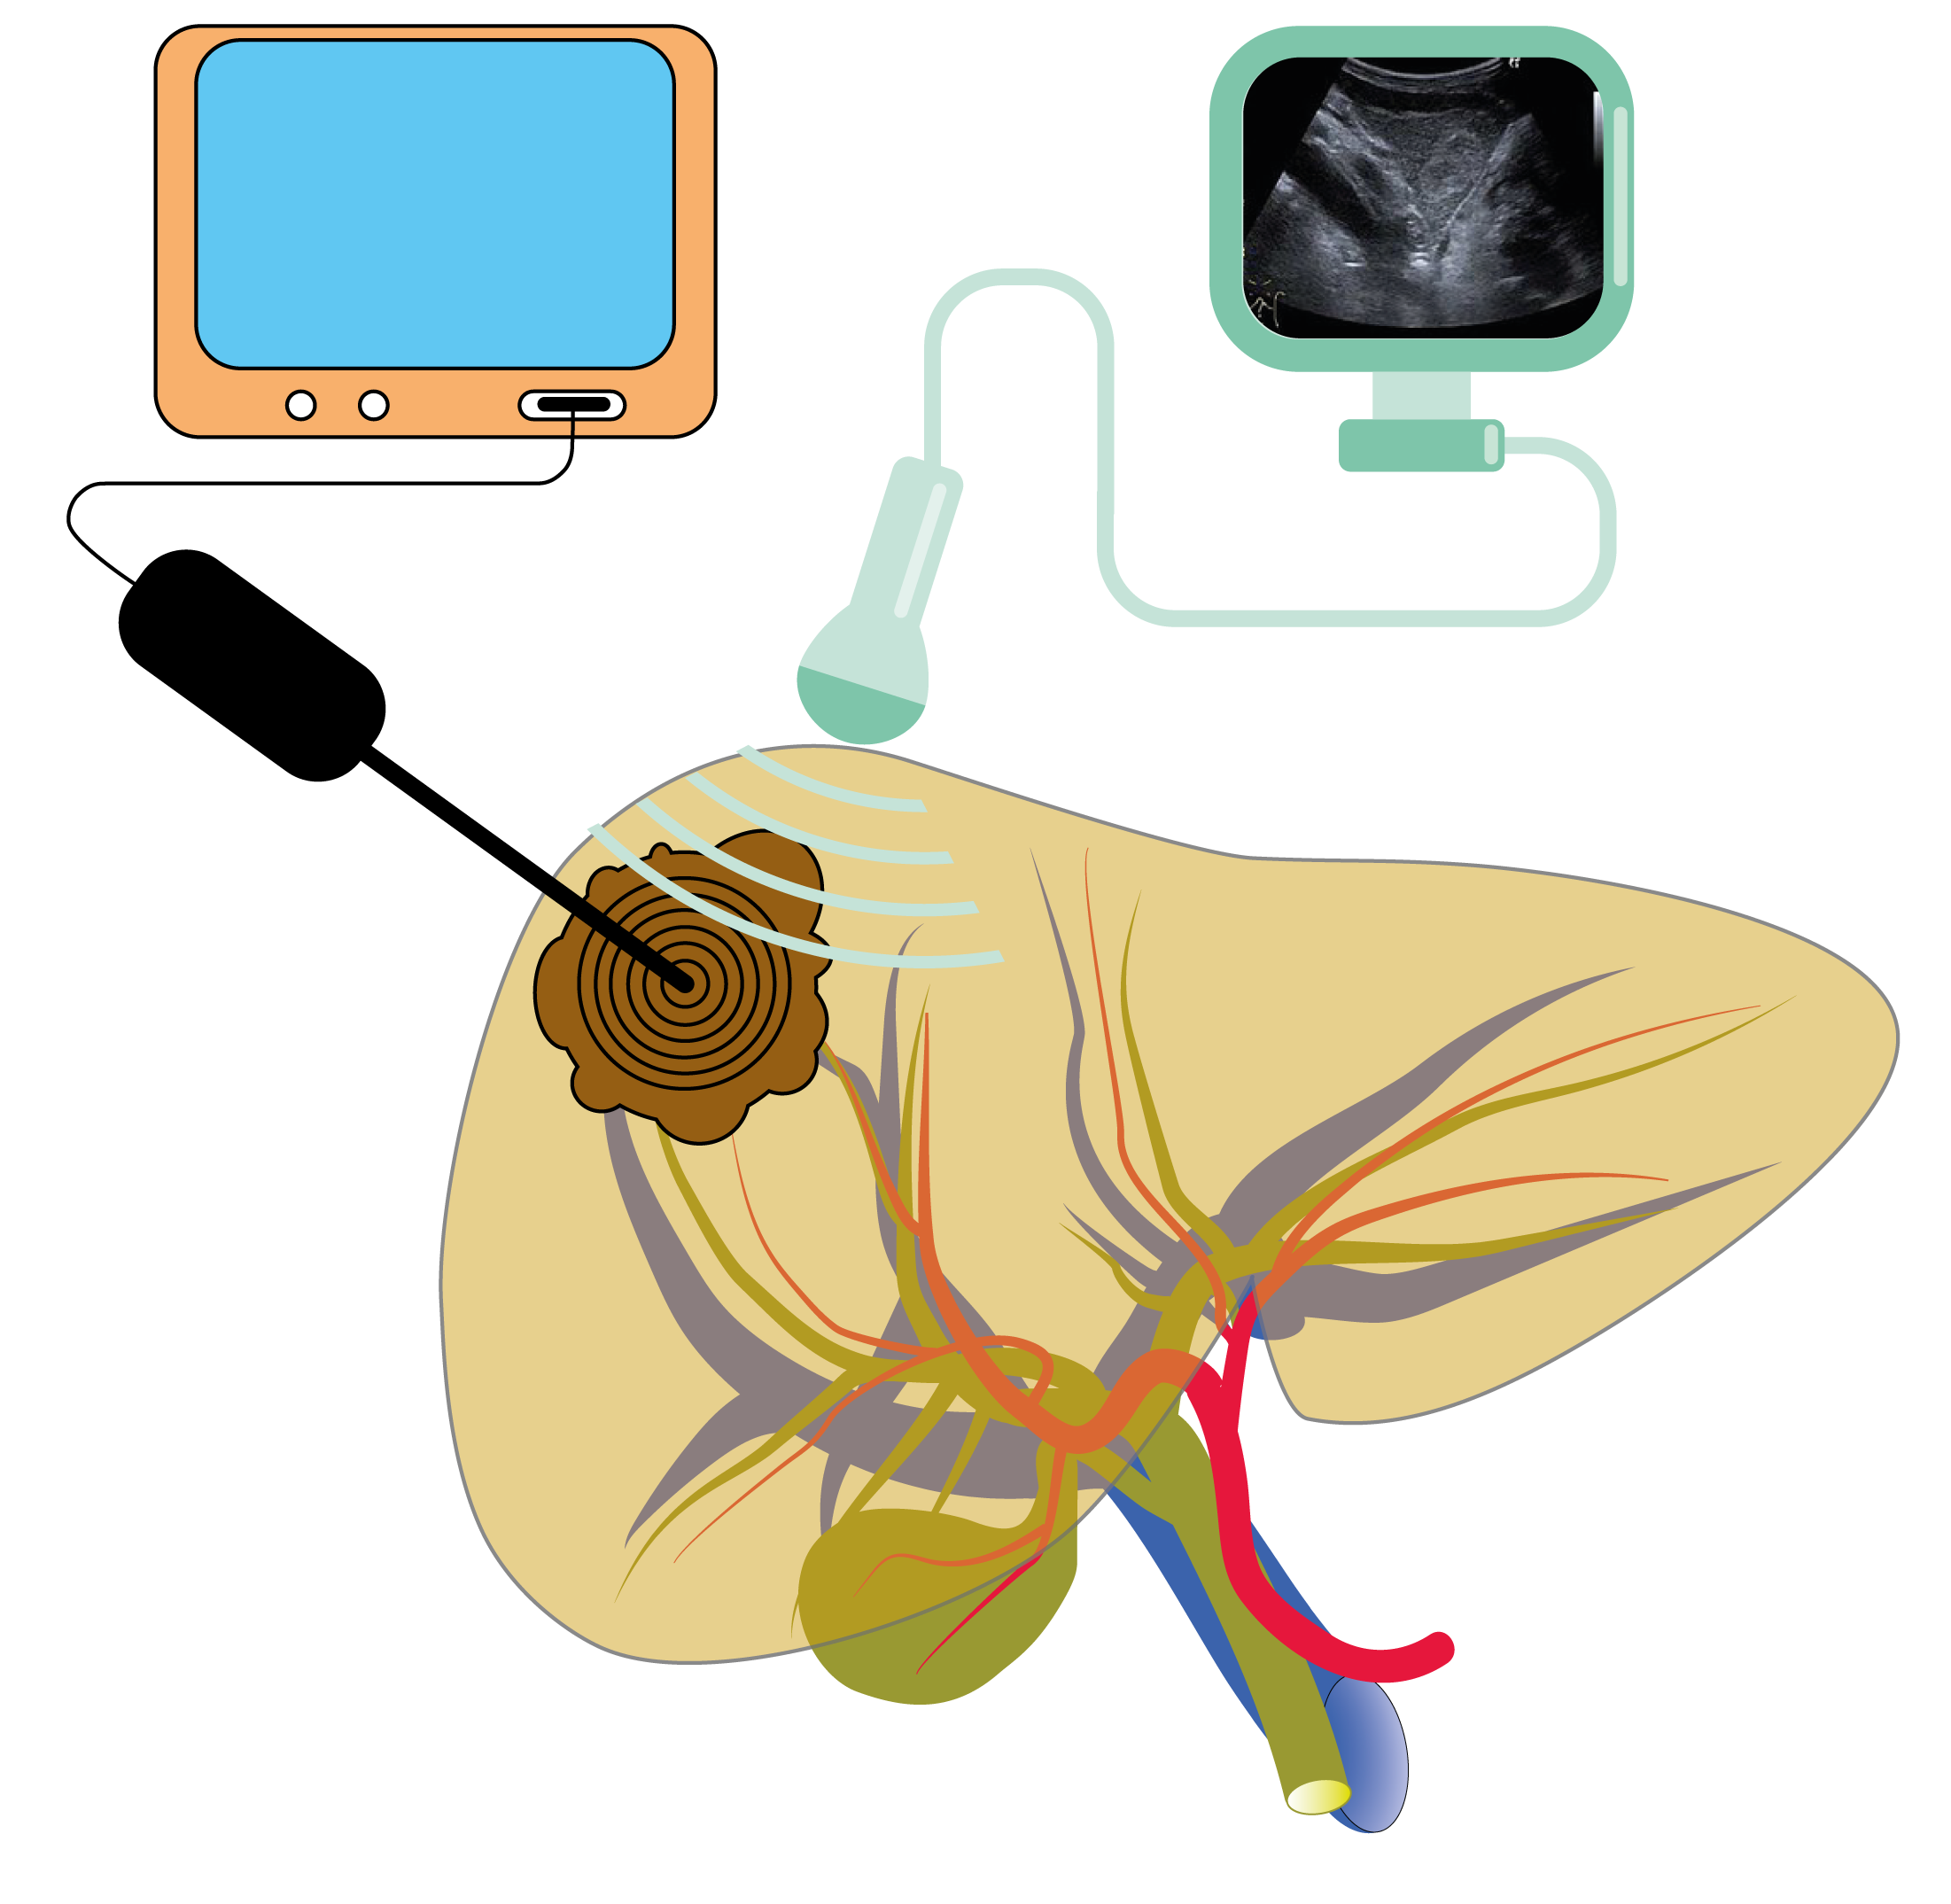
\includegraphics[width=\linewidth]{Figures/US procedures_Ablation.png}
            \caption{Високочастотна абляція пухлини. Під дією змінного тока високої частоти на кінці введеного під контролем ультразвуку електрода вогнище піддається термічній деструкції }
            \label{fig:goalbladder}
        \end{marginfigure}
        
        \item пункція та дренування кіст - евакуація вмісту кісти під УЗ-контролем та встановлення дренажної трубки в її порожнину за необхідності
        
        \begin{marginfigure}%
            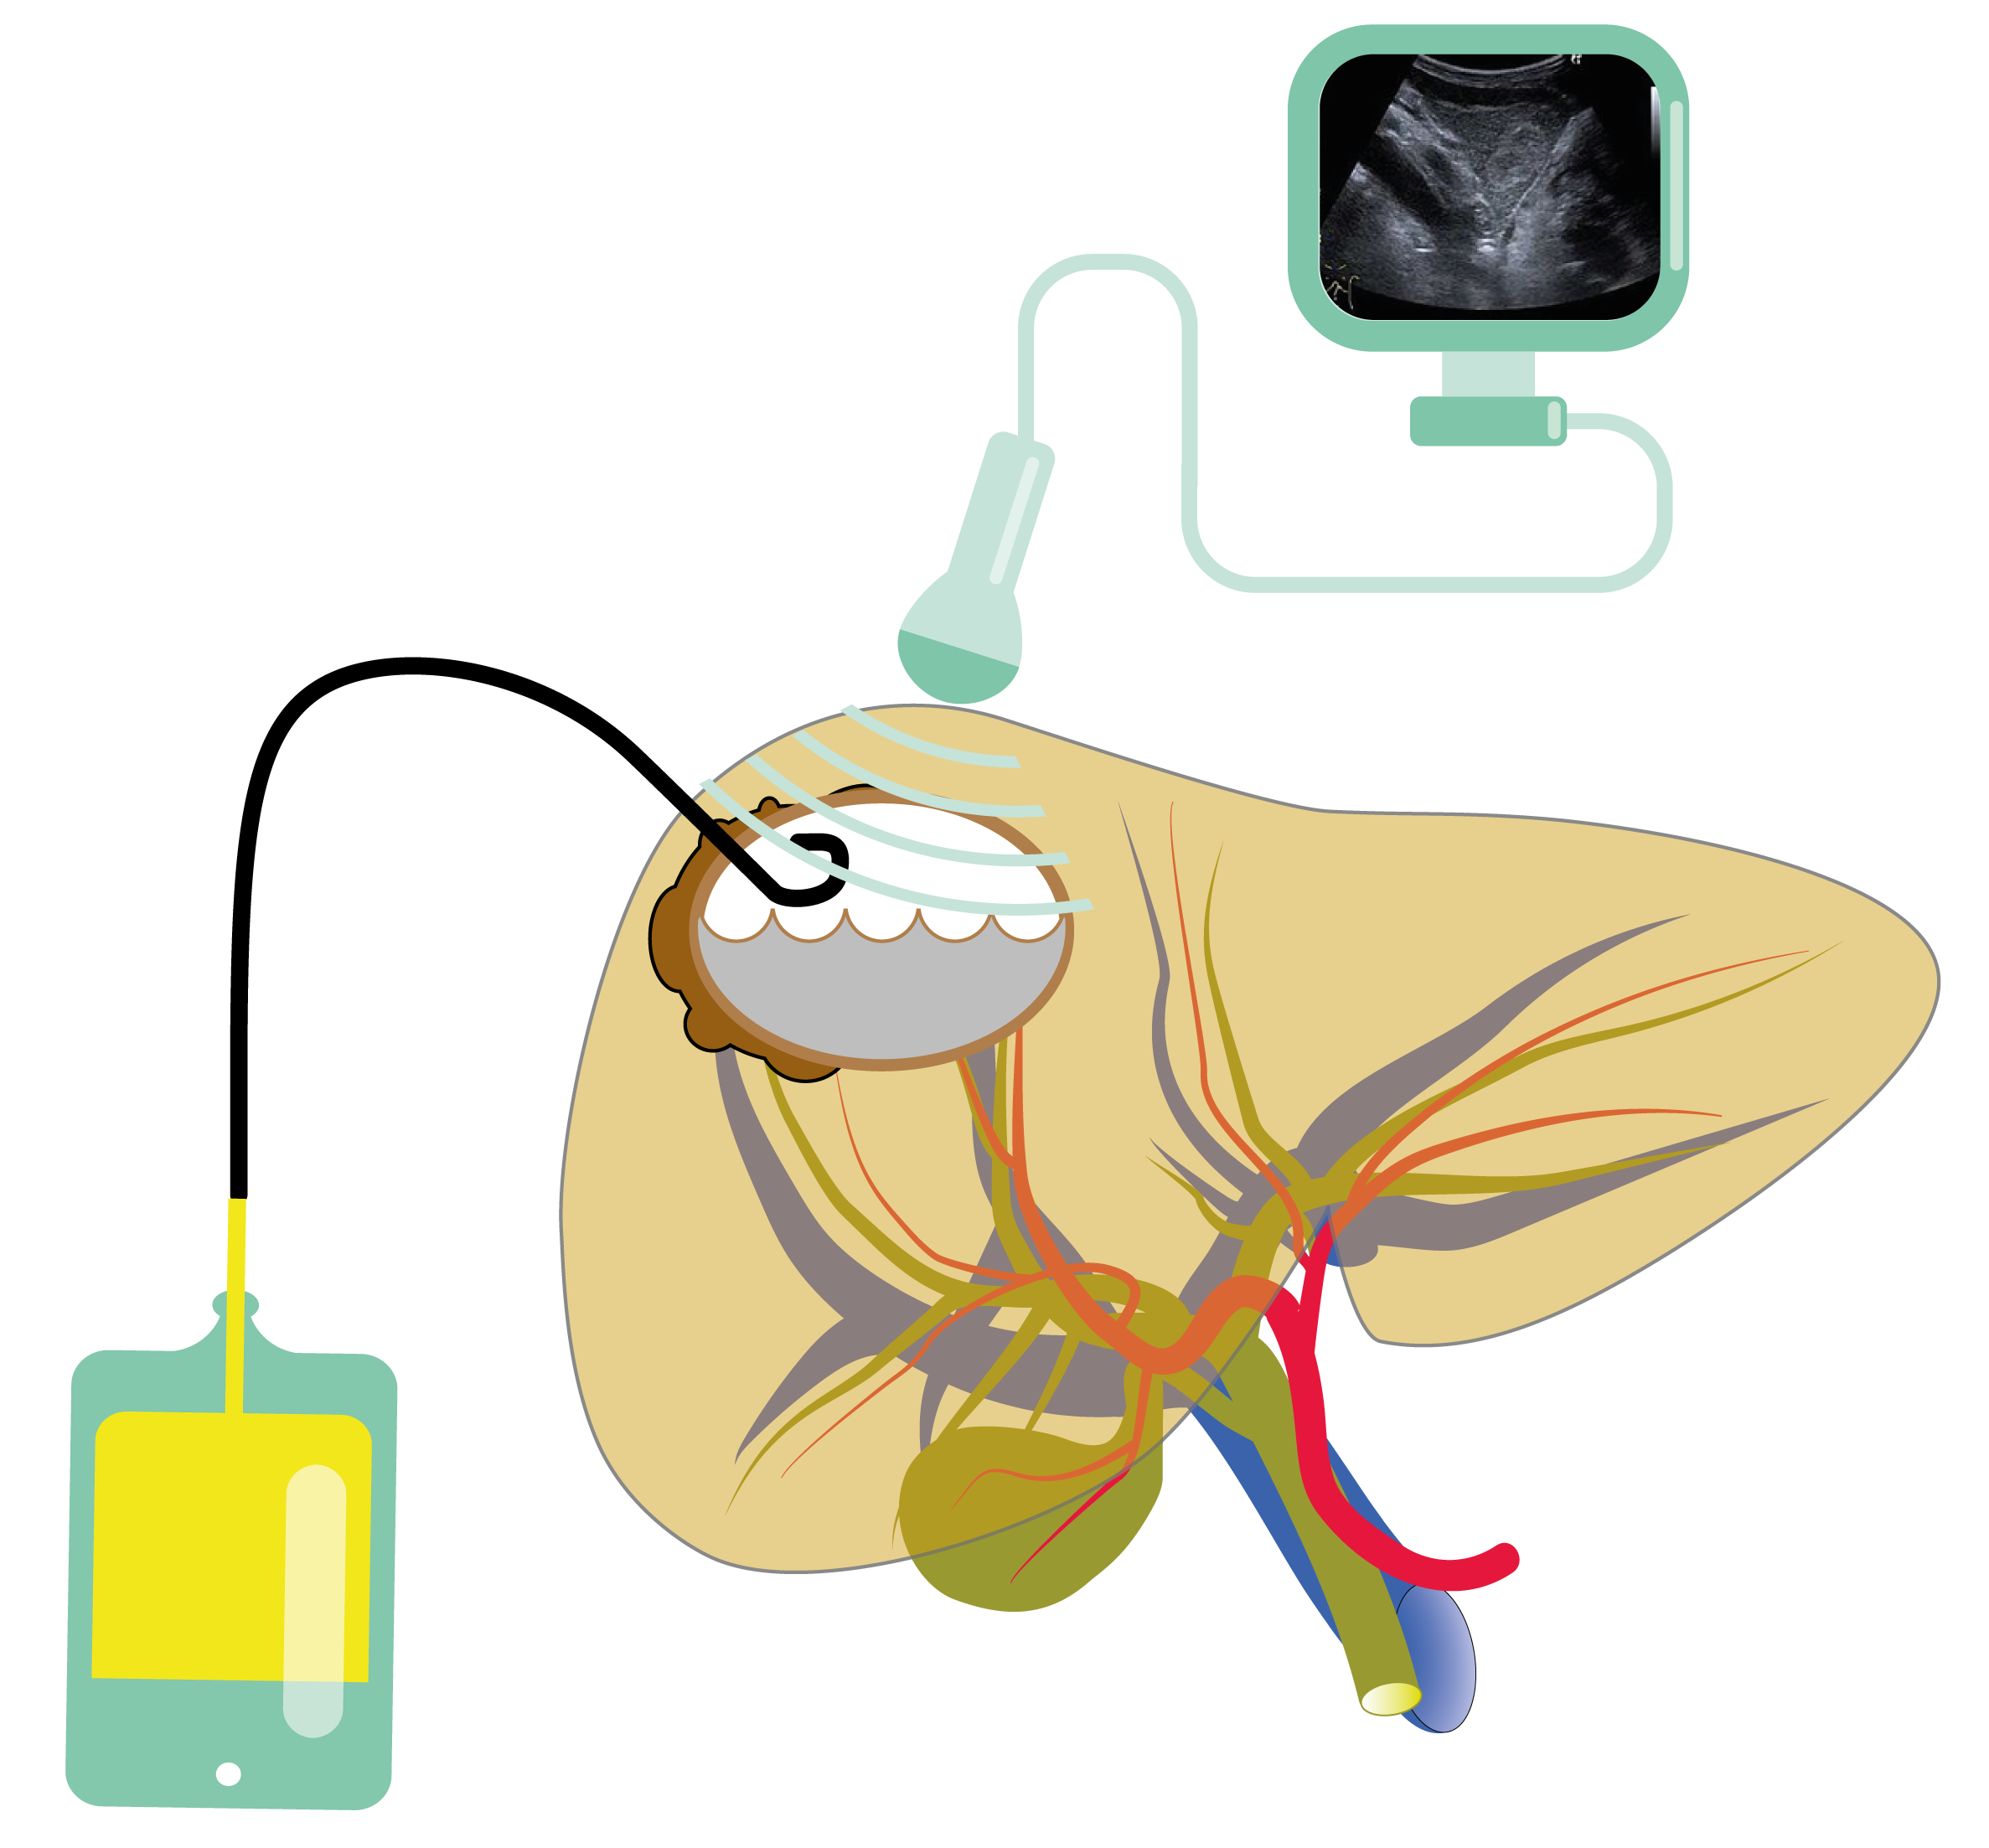
\includegraphics[width=\linewidth]{Figures/US procedures_Drain.png}
            \caption{Дренування абсцесу печінки під контролем ультразвуку}
            \label{fig:goalbladder}
        \end{marginfigure}
        
        
        
        \item біопсія печінки - взяття ділянки тканини печінки або пухлини для подальшого гістологічного дослідження. Використовується для постановки або уточнення діагнозу. Може бути виконана в 2 варіантах - пункційному (під УЗ-контролем) та лапароскопічному (під час діагностичної лапароскопії)
        
        \begin{marginfigure}%
            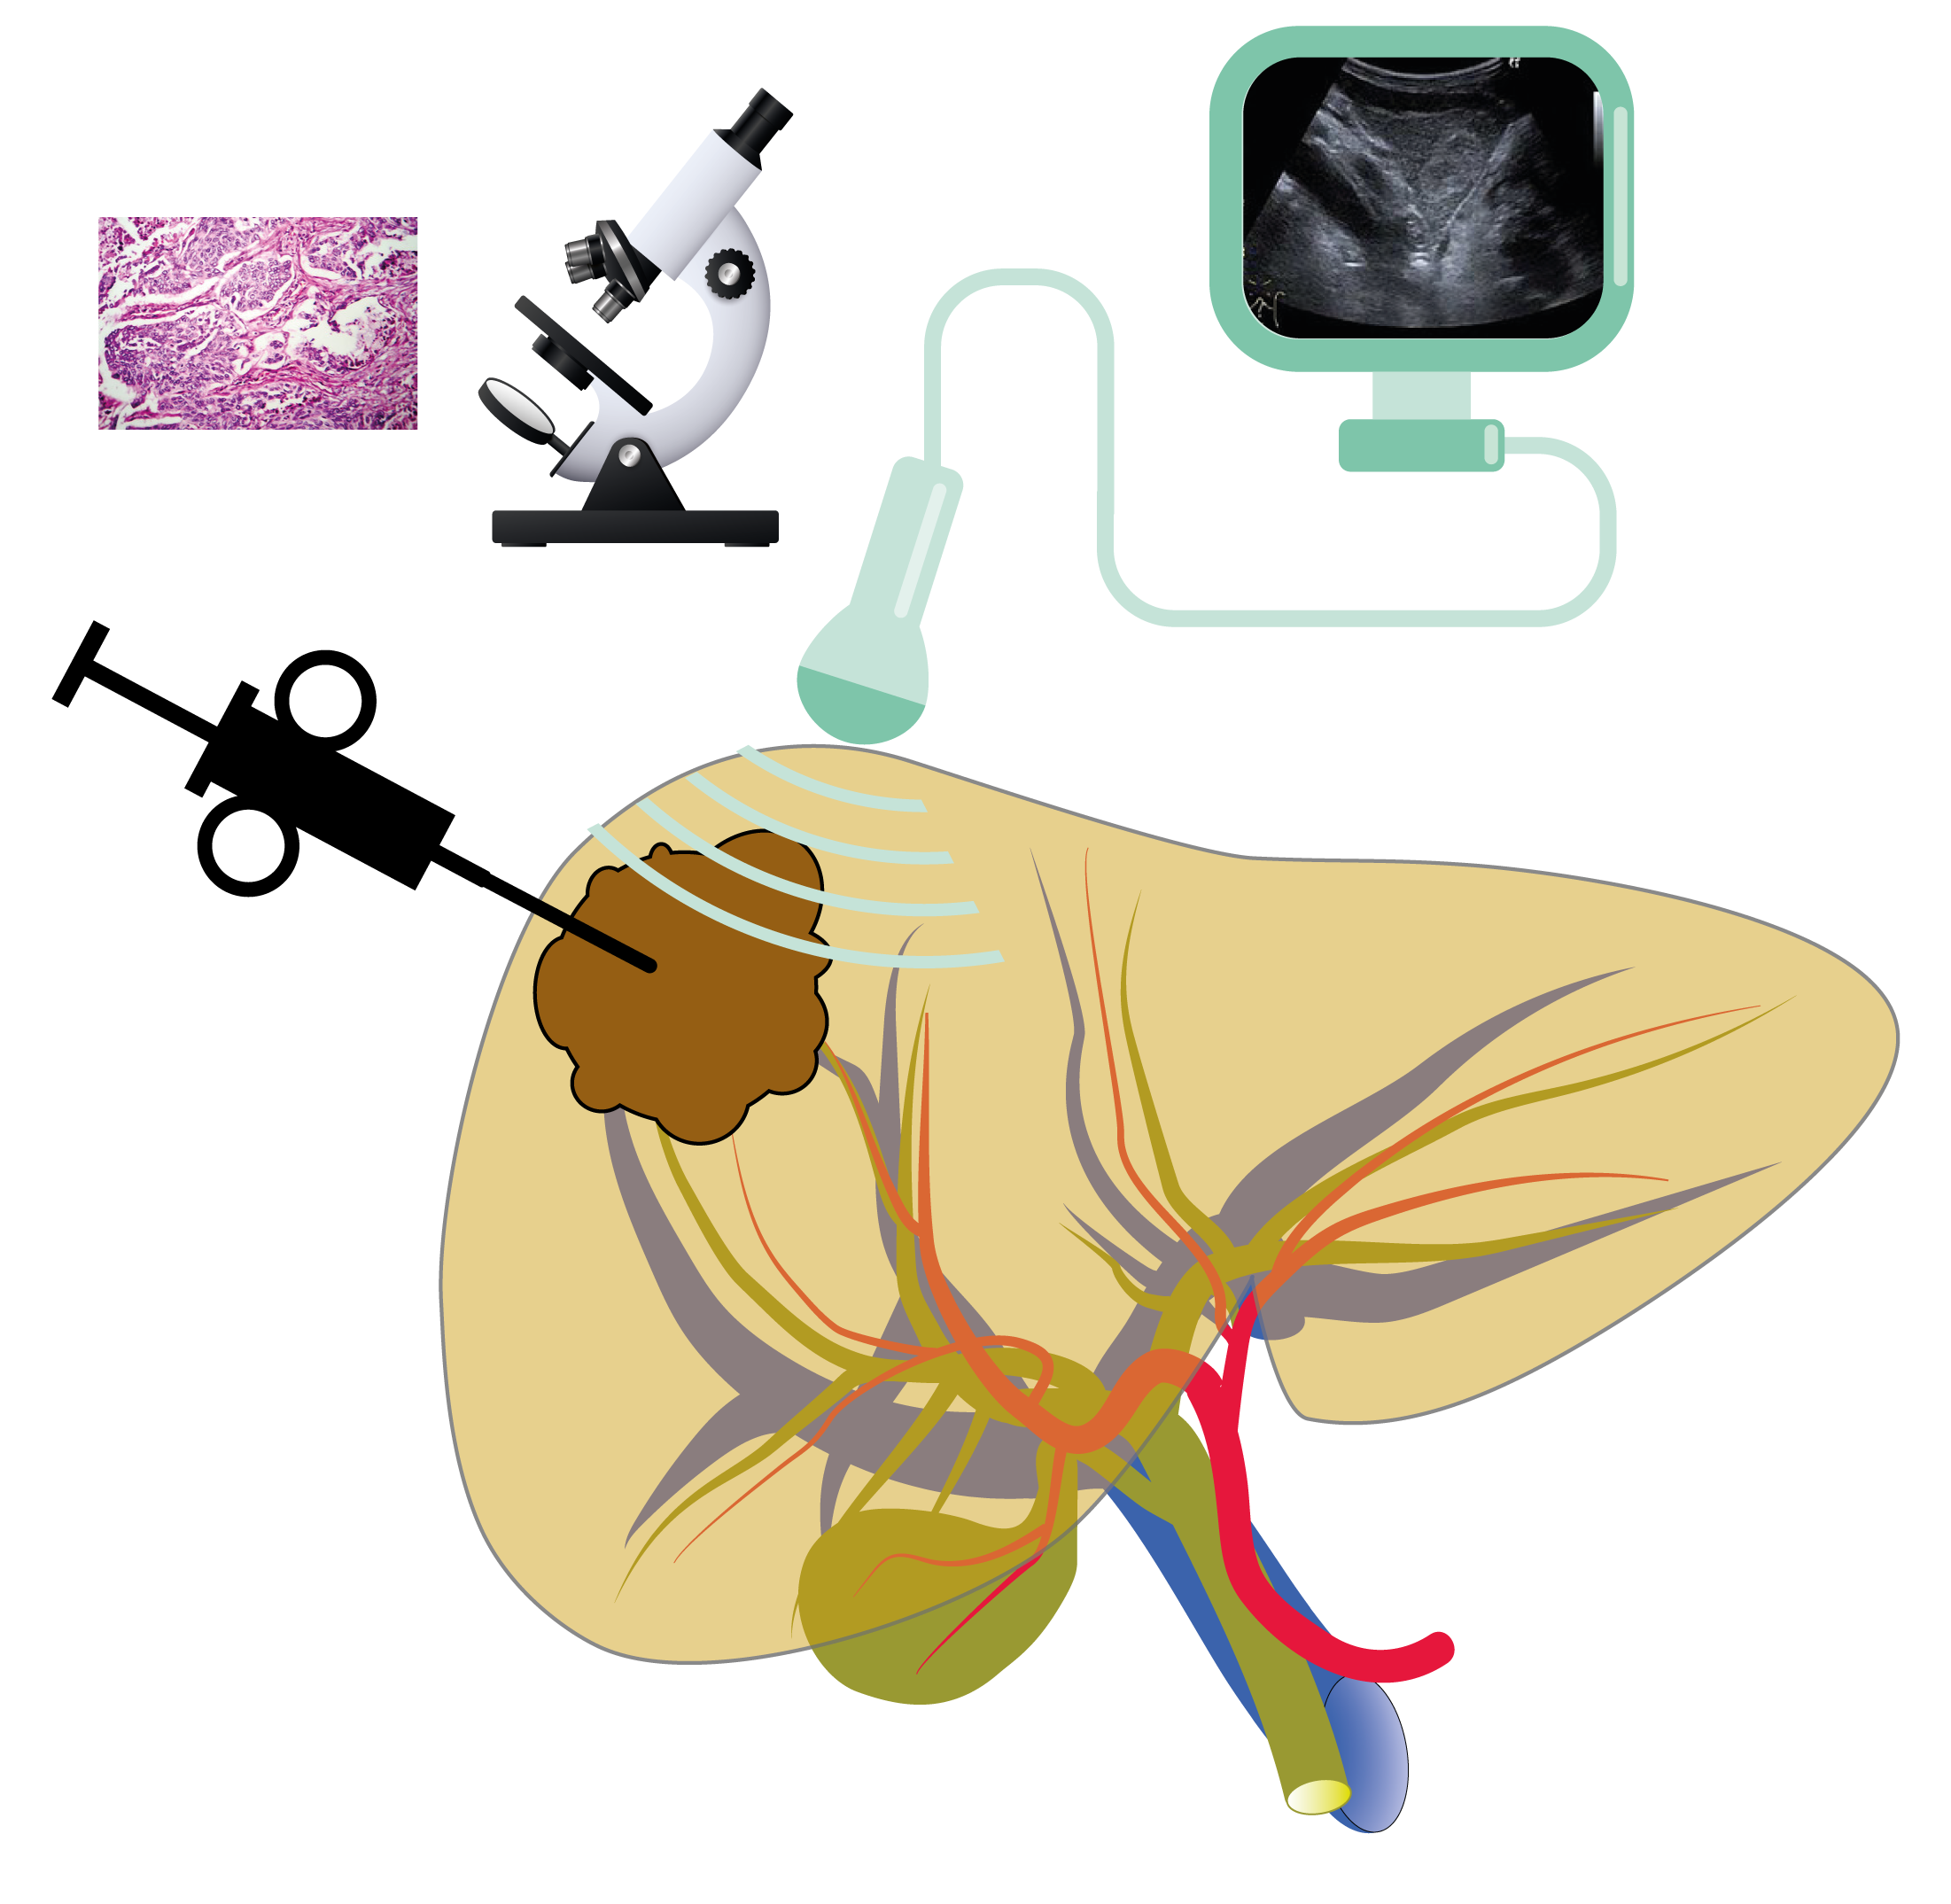
\includegraphics[width=\linewidth]{Figures/US procedures_Biopsy.png}
            \caption{Взяття ділянки пухлини біопсійною голкою під контролем ультразвуку для уточнення діагнозу}
            \label{fig:goalbladder}
        \end{marginfigure}
        
    \end{itemize}
	\item Ендобіліарні, рентгенконтрольовані втручання
	\begin{itemize}
	    \item зовнішнє дренування жовчних шляхів - процедура, під час якої в просвіт жовчного протоку через шкіру встановлюється дренажна трубка по якій далі відходить жовч. Використовується для тимчасової коррекції механічної жовтяниці перед операцією
	    
	    \begin{marginfigure}%
            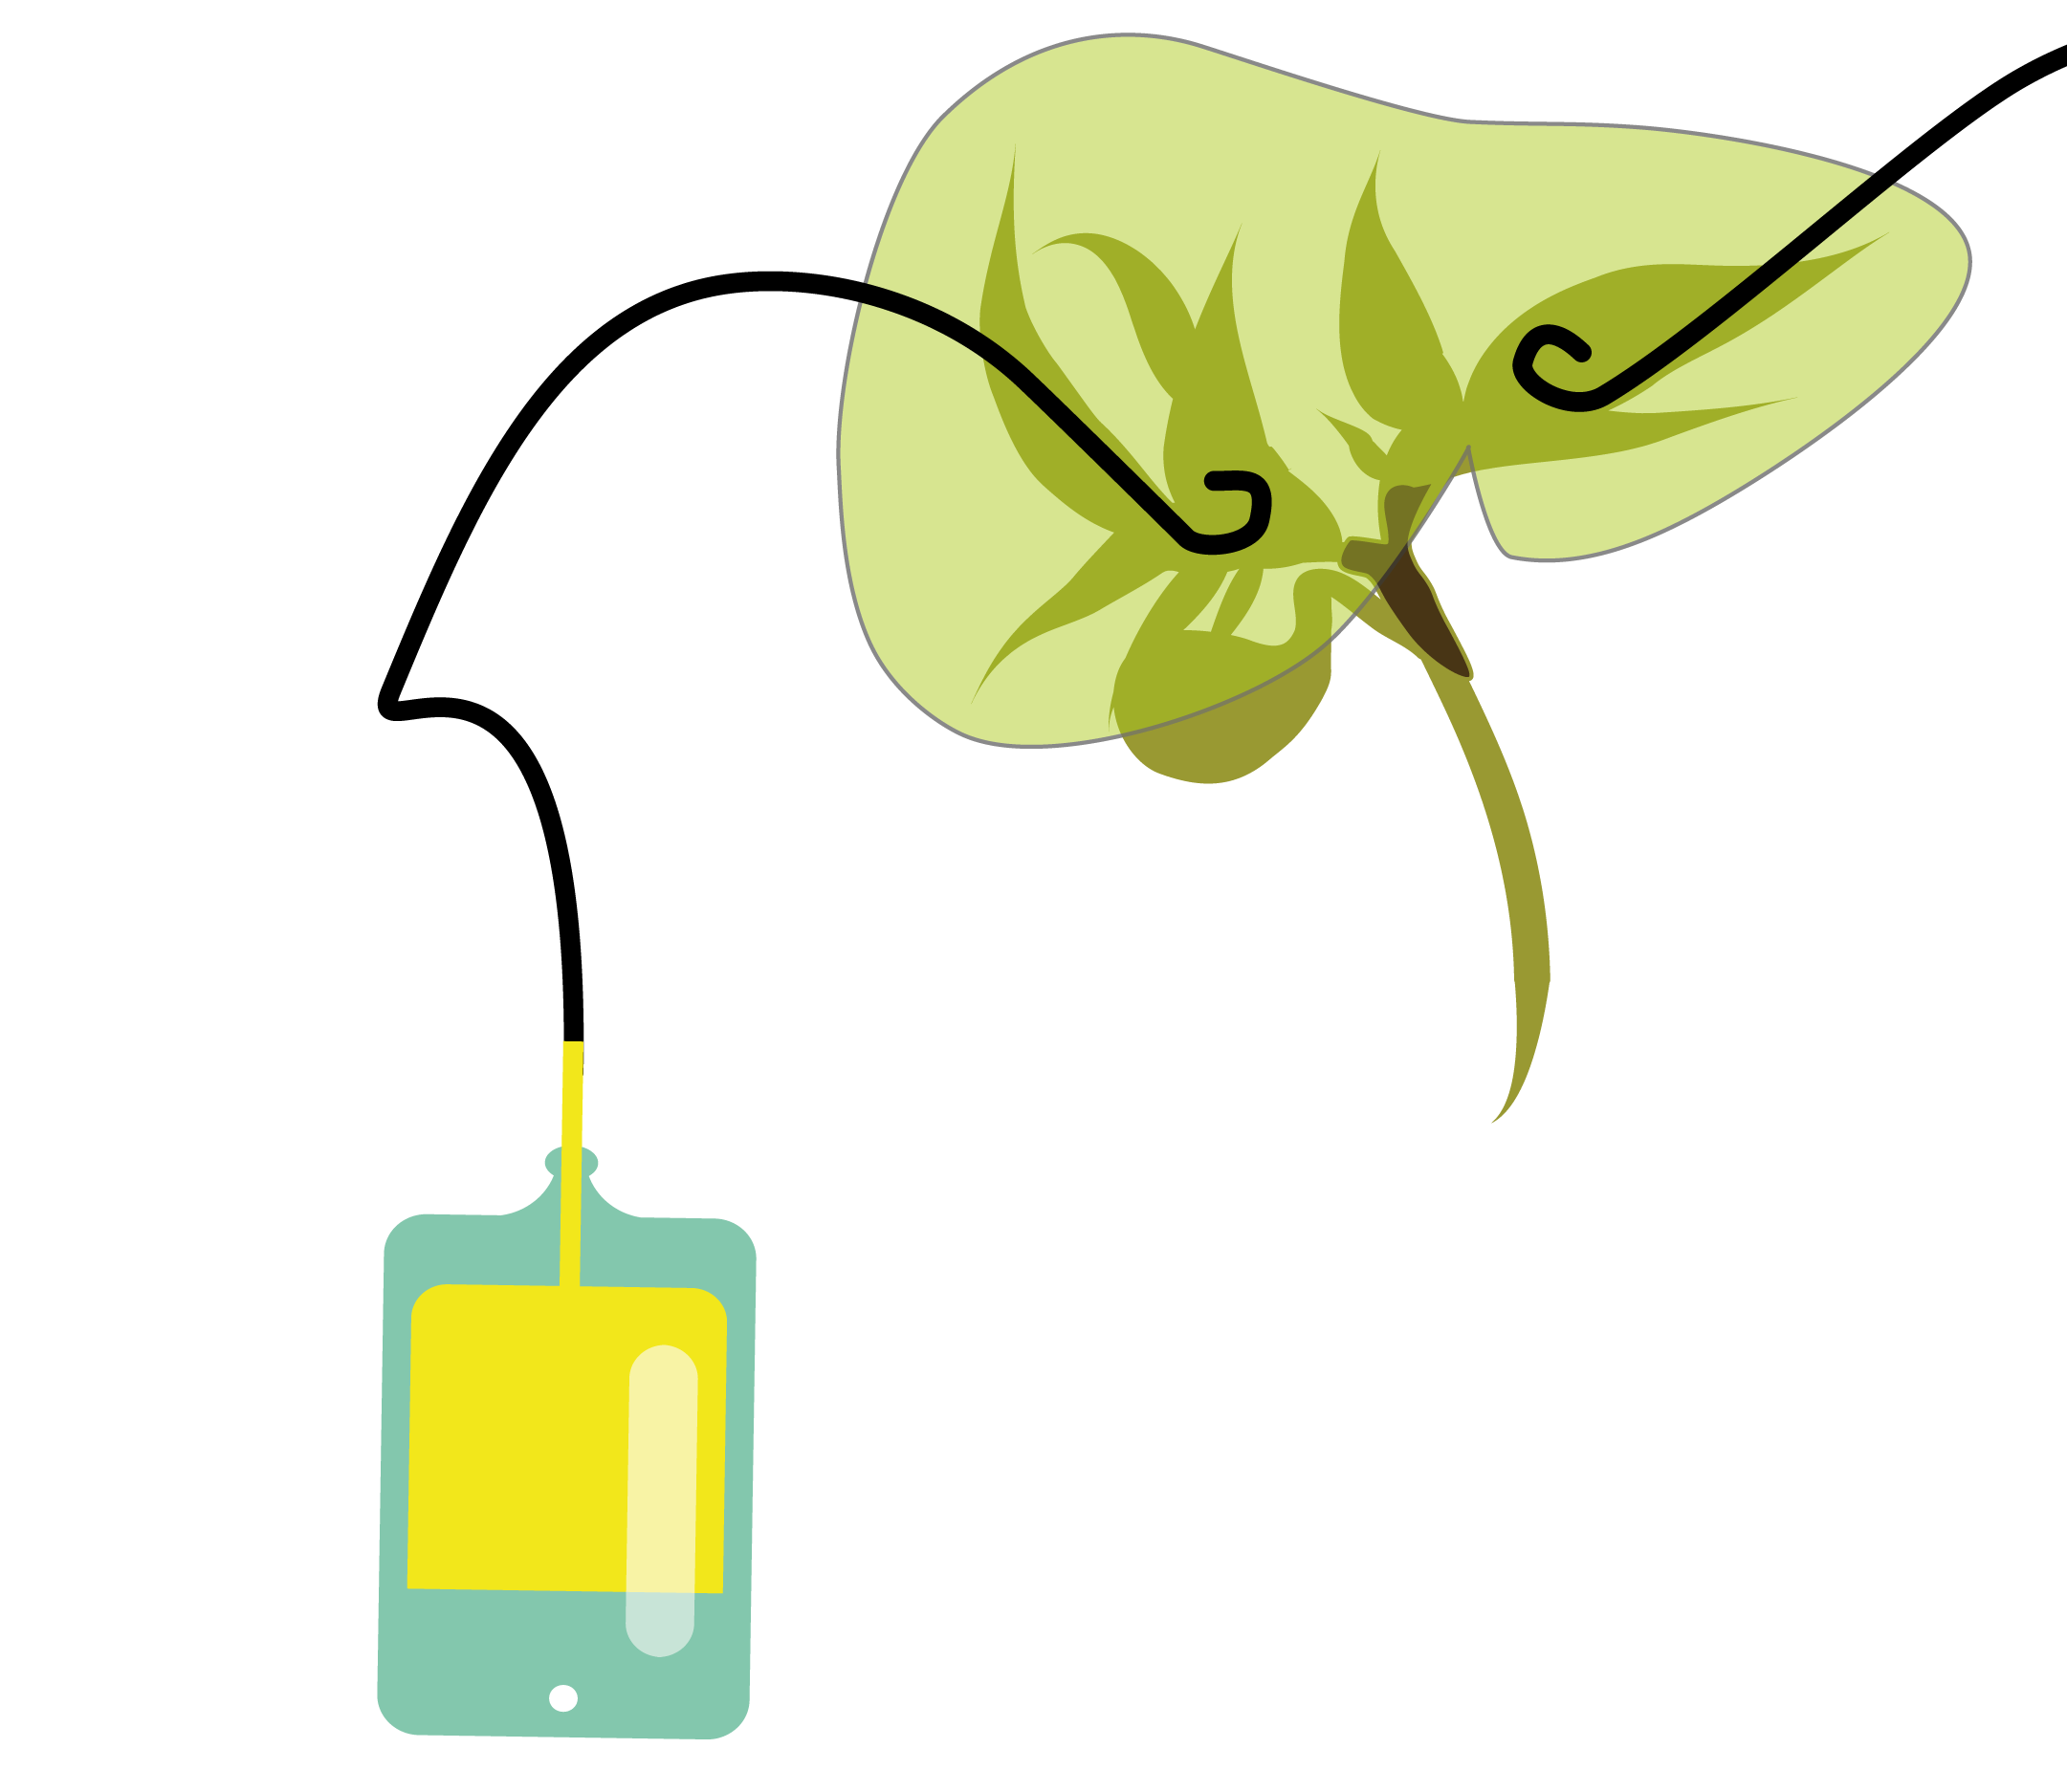
\includegraphics[width=\linewidth]{Figures/PTBD_Liver with drain.png}
            \caption{Встановлення черезшкірних черезпечінкових дренажів жовчних протоків під рентген-контролем для розрішення механічної жовтяниці внаслідок пухлинного процесу}
            \label{fig:goalbladder}
        \end{marginfigure}
	    
	    \item стентування жовчних протоків - процедура, під час якої в просвіт жовчного протоку встановлюється стент - спеціальний постійний розширювач, що дозволяє жовчі проходити повз механічну перепону. Використовується для постійної коррекції механічної жовтяницї
	    
	    \begin{marginfigure}%
            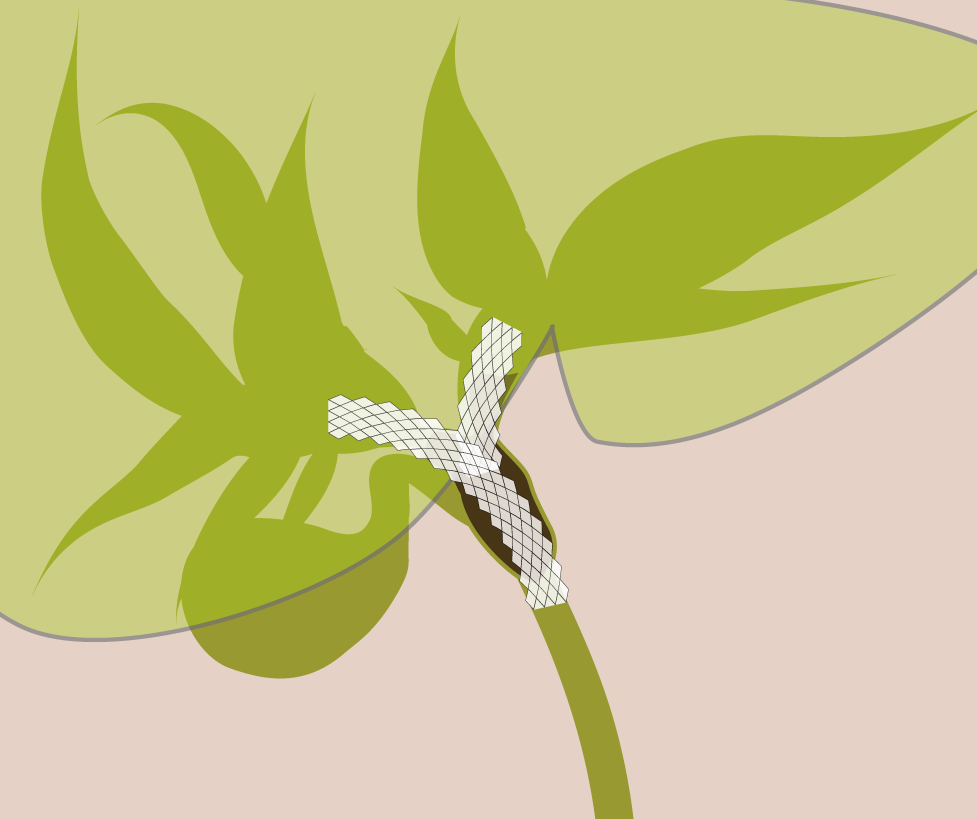
\includegraphics[width=\linewidth]{Figures/Bile duct stent_Stent.png}
            \caption{Встановлення встановлення ендобіліарного стенту для відновлення прохідності жовчних протоків під рентген-контролем}
            \label{fig:goalbladder}
        \end{marginfigure}
	    
	    \item ендоскопічна ретроградна холангіопанкреатографія - методика діагностики та лікування ураженнь жовчних шляхів за допомогою ендоскопа
	\end{itemize}
\end{itemize}  
\chapter{Трансплантація печінки}

\section{Що таке трансплантація печінки?}

Транспалнтація печінки - це високотехнологічне оперативне втручання, яке полягає у заміні хворої печінки пацієнта на здорову печінку (або частину печінки) донора. 

Після операції пацієнт пожиттєво отримує препарати, які запобігають відторгненню трансплантованого органу.

\begin{tcolorbox}[width=\textwidth,colback=yellow!5!white,colframe=yellow!75!black]    
Реципієнт - людина, якій пересаджують частину печінки
\end{tcolorbox}    

\begin{tcolorbox}[width=\textwidth,colback=yellow!5!white,colframe=yellow!75!black]    
Донор - людина, чию печінку або її частину пересаджують
\end{tcolorbox}    

\section{При яких захворюваннях показана трансплантація печінки?}

Трансплантації печінки показана при кінцевих стадіях захворювань печінки. Найчастіше це цироз печінки в наслідок вірусних гепатитів, аутоімунних захворюваннь печінки, вроджених патологій (біліарна атрезія та ін.), а також деяких нерезектабельних пухлин печінки та при гострій печінковій недостатності.


\section{Які види трансплантації печінки існують?}

За типом донора трансплантація може бути:
\begin{itemize}
    \item трупною, коли у людини з смертю мозку виконують забор цілої печінки
    \item від живого родинного донора, коли частину печінки для трансплантації беруть у живої людини, родича пацієнта 
\end{itemize}

\begin{figure}
  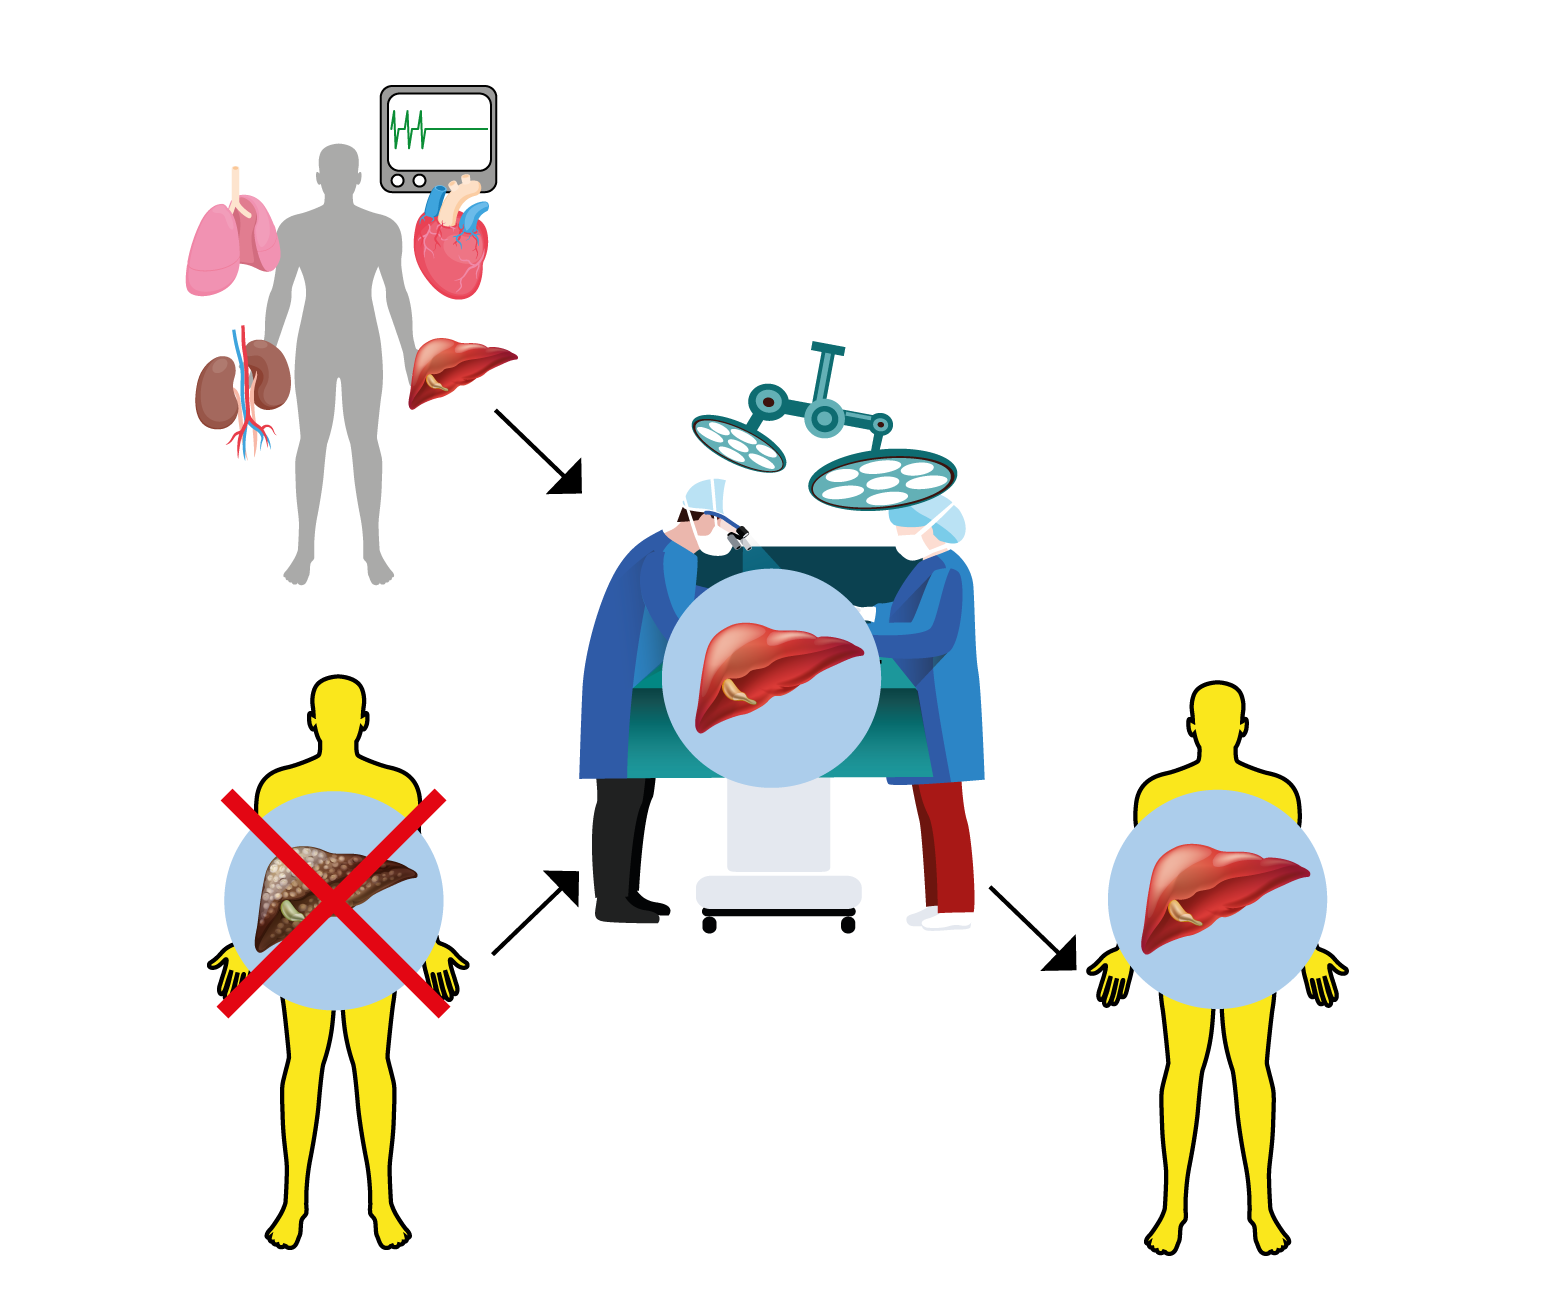
\includegraphics[width=\linewidth]{Figures/LTx-simple_DDLT.png}
%  \checkparity This is an \pageparity\ page.%
  \caption{Трансплантація печінки від трупного донора. В разі отримання згоди від родичів людини із встановленою смертю мозку їй виконують мультиорганний забор, після чого вилучені органи пересаджують ховрому.}
  \label{fig:ddlt}
  %\zsavepos{pos:textfig}
\end{figure}

\begin{figure}
  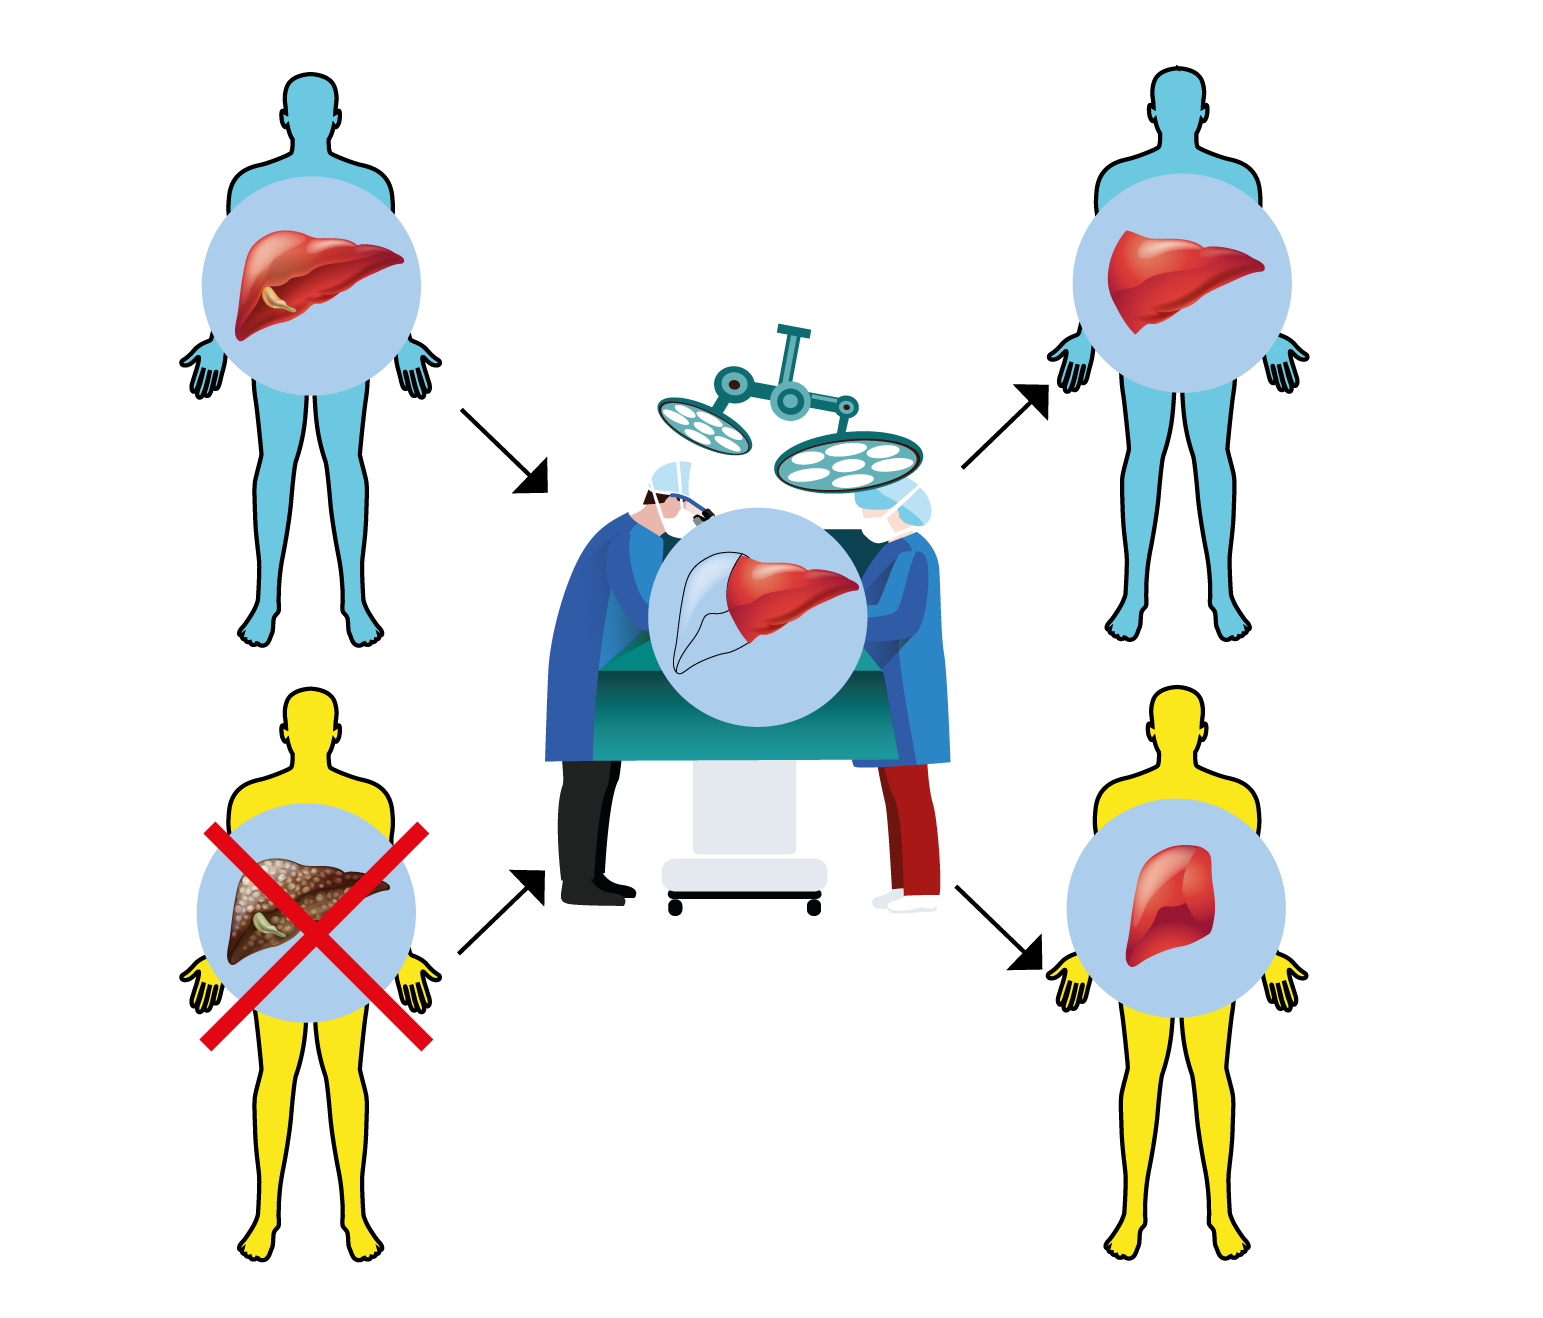
\includegraphics[width=\linewidth]{Figures/LTx-simple_LDLT.png}
%  \checkparity This is an \pageparity\ page.%
  \caption{Трансплантація печінки від живого родинного донора. Родич хворого донує йому частину своєї печінки.}
  \label{fig:ldlt}
  %\zsavepos{pos:textfig}
\end{figure}

Під час забору частини печінки у живого донора його печінку розділяють на дві функціонуючі частини. Одну з них трансплантують реципієнту на те ж місце де знаходилась  печінка, іншу залишають донору.


\section{Хто може бути живим родинним донором печінки?}

Згідно Закону України від 17.05.2018 № 2427-VIII Про застосування трансплантації анатомічних матеріалів людині, донором печінки можуть бути близькі родичі та члени сім’ї, до яких відносяться: чоловік, дружина, батько, мати, вітчим, мачуха, син, дочка, пасинок, падчерка, рідний брат, рідна сестра, двоюрідний брат, двоюрідна сестра, рідна тітка, рідний дядько, рідний племінник, рідна племінниця, дід, баба, прадід, прабаба, внук, внучка, правнук, правнучка, усиновлювач чи усиновлений, опікун чи піклувальник, особа, яка перебуває під опікою або піклуванням, а також особи, які спільно проживають, пов’язані спільним побутом і мають взаємні права та обов’язки, у тому числі особи, які спільно проживають, але не перебувають у шлюбі.



\section{Як відбувається процес підготовки до родинної трансплантації печінки?}

Як трансплантація печінки так і резекція печінки у донора є складними високотехнологічними операціями, тому для їх виконання необхідна ретельна передопераційна підготовка та всебічне поглиблене обстеження обох пацієнтів. В протокол обстеження обов’язково входять комп’ютерна томографія, магнітно-резонансна томографія, колоноскопія, лабораторне дослідження показників крові, та інші дослідження. Після обстеження пацієнти вносяться в лист очікування оперативного втручання
%\chapter{Порядок підготовки та проведення операції на печінці}

\section{Яке обстеження необхідне для проведення операцій на печінці?}

\section{Як відбувається планова підготовка до оперативного втручання?}

\section{Яким чином проходить післяопераційний період?}

%\chapter{The Design of Tufte's Books}

\bigskip
\begin{minipage}{\textwidth}
\begin{center}
\begin{tabular}{lcccc}
\toprule
 & \multicolumn{4}{c}{Books} \\
\cmidrule(l){2-5} 
Page content & \vdqi & \ei & \ve & \be \\
\midrule
Blank half title page & \hangp{1} & \hangp{1} & \hangp{1} & \hangp{1} \\
Frontispiece\footnotemark{}
  & \hangp{2} & \hangp{2} & \hangp{2} & \hangp{2} \\
Full title page & \hangp{3} & \hangp{3} & \hangp{3} & \hangp{3} \\
Copyright page & \hangp{4} & \hangp{4} & \hangp{4} & \hangp{4} \\
Contents & \hangp{5} & \hangp{5} & \hangp{5} & \hangp{5} \\
%Blank & -- & \hangp{6} & \hangp{6} & \hangp{6} \\
Dedication & \hangp{6} & \hangp{7} & \hangp{7} & 7 \\
%Blank & -- & \hangp{8} & -- & \hangp{8} \\
Epigraph & -- & -- & \hangp{8} & -- \\
Introduction & \hangp{7} & \hangp{9} & \hangp{9} & 9 \\
\bottomrule
\end{tabular}
\end{center}
\end{minipage}
\vspace{-7\baselineskip}\footnotetext{The contents of this page vary from book to book.  In
  \vdqi this page is blank; in \ei and \ve this page holds a frontispiece;
  and in \be this page contains three epigraphs.}
\vspace{7\baselineskip}

\bigskip
The design of the front matter in Tufte's books varies slightly from the
traditional design of front matter.  First, the pages in front matter are
traditionally numbered with lowercase roman numerals (\eg, i, ii, iii,
iv,~\ldots).  Second, the front matter page numbering sequence is usually
separate from the main matter page numbering.  That is, the page numbers
restart at 1 when the main matter begins.  In contrast, Tufte has
enumerated his pages with arabic numerals that share the same page counting
sequence as the main matter.  

There are also some variations in design across Tufte's four books.  The
page opposite the full title page (labeled ``frontispiece'' in the above
table) has different content in each of the books.  In \VDQI, this page is
blank; in \EI and \VE, this page holds a frontispiece; and in \BE, this
page contains three epigraphs.

The dedication appears on page~6 in \vdqi (opposite the introduction), and
is placed on its own spread in the other books.  In \ve, an epigraph shares
the spread with the opening page of the introduction.

None of the page numbers (folios) of the front matter are expressed except in
\be, where the folios start to appear on the dedication page.

\newthought{The full title page} of each of the books varies slightly in
design.  In all the books, the author's name appears at the top of the
page, the title it set just above the center line, and the publisher is
printed along the bottom margin.  Some of the differences are outlined in
the following table.

\bigskip
\begin{center}
\footnotesize
\begin{tabular}{lllll}
\toprule
Feature & \vdqi & \ei & \ve & \be \\
\midrule
Author & & & & \\
\quad Typeface & serif   & serif   & serif   & sans serif \\
\quad Style    & italics & italics & italics & upright, caps \\
\quad Size     & 24 pt   & 20 pt   & 20 pt   & 20 pt \\
\addlinespace
Title & & & & \\
\quad Typeface & serif   & serif   & serif   & sans serif \\
\quad Style    & upright & italics & upright & upright, caps \\
\quad Size     & 36 pt   & 48 pt   & 48 pt   & 36 pt \\
\addlinespace
Subtitle & & & & \\
\quad Typeface & \na     & \na     & serif   & \na \\
\quad Style    & \na     & \na     & upright & \na \\
\quad Size     & \na     & \na     & 20 pt   & \na \\
\addlinespace
Edition & & & & \\
\quad Typeface & sans serif    & \na  & \na  & \na \\
\quad Style    & upright, caps & \na  & \na  & \na \\
\quad Size     & 14 pt         & \na  & \na  & \na \\
\addlinespace
Publisher & & & & \\
\quad Typeface & serif   & serif   & serif   & sans serif \\
\quad Style    & italics & italics & italics & upright, caps \\
\quad Size     & 14 pt   & 14 pt   & 14 pt   & 14 pt \\
\bottomrule
\end{tabular}
\end{center}

\begin{figure*}[p]
\fbox{\includegraphics[width=0.45\linewidth]{Figures/vdqi-title.pdf}}
\hfill
\fbox{\includegraphics[width=0.45\linewidth]{Figures/ei-title.pdf}}
\\\vspace{\baselineskip}
\fbox{\includegraphics[width=0.45\linewidth]{Figures/ve-title.pdf}}
\hfill
\fbox{\includegraphics[width=0.45\linewidth]{Figures/be-title.pdf}}
\end{figure*}

\newthought{The tables of contents} in Tufte's books give us our first
glimpse of the structure of the main matter.  \VDQI is split into two
parts, each containing some number of chapters.  His other three books only
contain chapters---they're not broken into parts.

\begin{figure*}[p]\index{table of contents}
\fbox{\includegraphics[width=0.45\linewidth]{Figures/vdqi-contents.pdf}}
\hfill
\fbox{\includegraphics[width=0.45\linewidth]{Figures/ei-contents.pdf}}
\\\vspace{\baselineskip}
\fbox{\includegraphics[width=0.45\linewidth]{Figures/ve-contents.pdf}}
\hfill
\fbox{\includegraphics[width=0.45\linewidth]{Figures/be-contents.pdf}}
\end{figure*}


\section{Typefaces}\label{sec:typefaces1}\index{typefaces}
\index{fonts|see{typefaces}}

Tufte's books primarily use two typefaces: Bembo and Gill Sans.  Bembo is used
for the headings and body text, while Gill Sans is used for the title page and
opening epigraphs in \BE.

Since neither Bembo nor Gill Sans are available in default \LaTeX{}
installations, the \TL document classes default to using Palatino and
Helvetica, respectively.  In addition, the Bera Mono typeface is used for
\texttt{monospaced} type.

The following font sizes are defined by the \TL classes:

\begin{table}[h]\index{typefaces!sizes}
  \footnotesize%
  \begin{center}
    \begin{tabular}{lccl}
      \toprule
      \LaTeX{} size & Font size & Leading & Used for \\
      \midrule
      \verb+\tiny+         &  5 &  6 & sidenote numbers \\
      \verb+\scriptsize+   &  7 &  8 & \na \\
      \verb+\footnotesize+ &  8 & 10 & sidenotes, captions \\
      \verb+\small+        &  9 & 12 & quote, quotation, and verse environments \\
      \verb+\normalsize+   & 10 & 14 & body text \\
      \verb+\large+        & 11 & 15 & \textsc{b}-heads \\
      \verb+\Large+        & 12 & 16 & \textsc{a}-heads, \textsc{toc} entries, author, date \\
      \verb+\LARGE+        & 14 & 18 & handout title \\
      \verb+\huge+         & 20 & 30 & chapter heads \\
      \verb+\Huge+         & 24 & 36 & part titles \\
      \bottomrule
    \end{tabular}
  \end{center}
  \caption{A list of \LaTeX{} font sizes as defined by the \TL document classes.}
  \label{tab:font-sizes}
\end{table}

\section{Headings}\label{sec:headings1}\index{headings}

Tufte's books include the following heading levels: parts,
chapters,\sidenote{Parts and chapters are defined for the \texttt{tufte-book}
class only.}  sections, subsections, and paragraphs.  Not defined by default
are: sub-subsections and subparagraphs.

\begin{table}[h]
  \begin{center}
    \footnotesize%
    \begin{tabular}{lcr}
      \toprule
      Heading & Style & Size \\
      \midrule
      Part & roman & \measure{24}{36}{40} \\
      Chapter & italic & \measure{20}{30}{40} \\
      Section & italic & \measure{12}{16}{26} \\
      Subsection & italic & \measure{11}{15}{26} \\
      Paragraph & italic & 10/14 \\
      \bottomrule
    \end{tabular}
  \end{center}
  \caption{Heading styles used in \BE.}
  \label{tab:heading-styles}
\end{table}

\paragraph{Paragraph} Paragraph headings (as shown here) are introduced by
italicized text and separated from the main paragraph by a bit of space.

\section{Environments}

The following characteristics define the various environments:


\begin{table}[h]
  \begin{center}
    \footnotesize%
    \begin{tabular}{lcl}
      \toprule
      Environment & Font size & Notes \\
      \midrule
      Body text & \measure{10}{14}{26} & \\
      Block quote & \measure{9}{12}{24} & Block indent (left and right) by \unit[1]{pc} \\
      Sidenotes & \measure{8}{10}{12} & Sidenote number is set inline, followed by word space \\
      Captions & \measure{8}{10}{12} &  \\
      \bottomrule
    \end{tabular}
  \end{center}
  \caption{Environment styles used in \BE.}
  \label{tab:environment-styles}
\end{table}


\chapter[On the Use of the tufte-book Document Class]{On the Use of the \texttt{tufte-book} Document Class}
\label{ch:tufte-book}

The \TL document classes define a style similar to the
style Edward Tufte uses in his books and handouts.  Tufte's style is known
for its extensive use of sidenotes, tight integration of graphics with
text, and well-set typography.  This document aims to be at once a
demonstration of the features of the \TL document classes
and a style guide to their use.

\section{Page Layout}\label{sec:page-layout}
\subsection{Headings}\label{sec:headings}\index{headings}
This style provides \textsc{a}- and \textsc{b}-heads (that is,
\Verb|\section| and \Verb|\subsection|), demonstrated above.

If you need more than two levels of section headings, you'll have to define
them yourself at the moment; there are no pre-defined styles for anything below
a \Verb|\subsection|.  As Bringhurst points out in \textit{The Elements of
Typographic Style},\cite{Bringhurst2005} you should ``use as many levels of
headings as you need: no more, and no fewer.''

The \TL classes will emit an error if you try to use
\linebreak\Verb|\subsubsection| and smaller headings.

% let's start a new thought -- a new section
\newthought{In his later books},\cite{Tufte2006} Tufte
starts each section with a bit of vertical space, a non-indented paragraph,
and sets the first few words of the sentence in \textsc{small caps}.  To
accomplish this using this style, use the \doccmddef{newthought} command:
\begin{docspec}
  \doccmd{newthought}\{In his later books\}, Tufte starts\ldots
\end{docspec}


\section{Sidenotes}\label{sec:sidenotes}
One of the most prominent and distinctive features of this style is the
extensive use of sidenotes.  There is a wide margin to provide ample room
for sidenotes and small figures.  Any \doccmd{footnote}s will automatically
be converted to sidenotes.\footnote{This is a sidenote that was entered
using the \texttt{\textbackslash footnote} command.}  If you'd like to place ancillary
information in the margin without the sidenote mark (the superscript
number), you can use the \doccmd{marginnote} command.\marginnote{This is a
margin note.  Notice that there isn't a number preceding the note, and
there is no number in the main text where this note was written.}

The specification of the \doccmddef{sidenote} command is:
\begin{docspec}
  \doccmd{sidenote}[\docopt{number}][\docopt{offset}]\{\docarg{Sidenote text.}\}
\end{docspec}

Both the \docopt{number} and \docopt{offset} arguments are optional.  If you
provide a \docopt{number} argument, then that number will be used as the
sidenote number.  It will change of the number of the current sidenote only and
will not affect the numbering sequence of subsequent sidenotes.

Sometimes a sidenote may run over the top of other text or graphics in the
margin space.  If this happens, you can adjust the vertical position of the
sidenote by providing a dimension in the \docopt{offset} argument.  Some
examples of valid dimensions are:
\begin{docspec}
  \ttfamily 1.0in \qquad 2.54cm \qquad 254mm \qquad 6\Verb|\baselineskip|
\end{docspec}
If the dimension is positive it will push the sidenote down the page; if the
dimension is negative, it will move the sidenote up the page.

While both the \docopt{number} and \docopt{offset} arguments are optional, they
must be provided in order.  To adjust the vertical position of the sidenote
while leaving the sidenote number alone, use the following syntax:
\begin{docspec}
  \doccmd{sidenote}[][\docopt{offset}]\{\docarg{Sidenote text.}\}
\end{docspec}
The empty brackets tell the \Verb|\sidenote| command to use the default
sidenote number.

If you \emph{only} want to change the sidenote number, however, you may
completely omit the \docopt{offset} argument:
\begin{docspec}
  \doccmd{sidenote}[\docopt{number}]\{\docarg{Sidenote text.}\}
\end{docspec}

The \doccmddef{marginnote} command has a similar \docarg{offset} argument:
\begin{docspec}
  \doccmd{marginnote}[\docopt{offset}]\{\docarg{Margin note text.}\}
\end{docspec}

\section{References}
References are placed alongside their citations as sidenotes,
as well.  This can be accomplished using the normal \doccmddef{cite}
command.\sidenote{The first paragraph of this document includes a citation.}

The complete list of references may also be printed automatically by using
the \doccmddef{bibliography} command.  (See the end of this document for an
example.)  If you do not want to print a bibliography at the end of your
document, use the \doccmddef{nobibliography} command in its place.  

To enter multiple citations at one location,\cite[-3\baselineskip]{Tufte2006,Tufte1990} you can
provide a list of keys separated by commas and the same optional vertical
offset argument: \Verb|\cite{Tufte2006,Tufte1990}|.  
\begin{docspec}
  \doccmd{cite}[\docopt{offset}]\{\docarg{bibkey1,bibkey2,\ldots}\}
\end{docspec}

\section{Figures and Tables}\label{sec:figures-and-tables}
Images and graphics play an integral role in Tufte's work.
In addition to the standard \docenvdef{figure} and \docenvdef{tabular} environments,
this style provides special figure and table environments for full-width
floats.

Full page--width figures and tables may be placed in \docenvdef{figure*} or
\docenvdef{table*} environments.  To place figures or tables in the margin,
use the \docenvdef{marginfigure} or \docenvdef{margintable} environments as follows
(see figure~\ref{fig:marginfig}):

\begin{marginfigure}%
  \includegraphics[width=\linewidth]{helix}
  \caption{This is a margin figure.  The helix is defined by 
    $x = \cos(2\pi z)$, $y = \sin(2\pi z)$, and $z = [0, 2.7]$.  The figure was
    drawn using Asymptote (\url{http://asymptote.sf.net/}).}
  \label{fig:marginfig}
\end{marginfigure}

\begin{docspec}
\textbackslash begin\{marginfigure\}\\
  \qquad\textbackslash includegraphics\{helix\}\\
  \qquad\textbackslash caption\{This is a margin figure.\}\\
  \qquad\textbackslash label\{fig:marginfig\}\\
\textbackslash end\{marginfigure\}\\
\end{docspec}

The \docenv{marginfigure} and \docenv{margintable} environments accept an optional parameter \docopt{offset} that adjusts the vertical position of the figure or table.  See the ``\nameref{sec:sidenotes}'' section above for examples.  The specifications are:
\begin{docspec}
  \textbackslash{begin\{marginfigure\}[\docopt{offset}]}\\
  \qquad\ldots\\
  \textbackslash{end\{marginfigure\}}\\
  \mbox{}\\
  \textbackslash{begin\{margintable\}[\docopt{offset}]}\\
  \qquad\ldots\\
  \textbackslash{end\{margintable\}}\\
\end{docspec}

Figure~\ref{fig:fullfig} is an example of the \docenv{figure*}
environment and figure~\ref{fig:textfig} is an example of the normal
\docenv{figure} environment.


\begin{figure*}[h]
  \includegraphics[width=\linewidth]{Figures/sine.pdf}%
  \caption{This graph shows $y = \sin x$ from about $x = [-10, 10]$.
  \emph{Notice that this figure takes up the full page width.}}%
  \label{fig:fullfig}%
\end{figure*}

\begin{figure}
  \includegraphics{Figures/Up-frontal liver.pdf}
%  \checkparity This is an \pageparity\ page.%
  \caption[Hilbert curves of various degrees $n$.][6pt]{Hilbert curves of various degrees $n$. \emph{Notice that this figure only takes up the main textblock width.}}
  \label{fig:textfig}
  %\zsavepos{pos:textfig}
\end{figure}

As with sidenotes and marginnotes, a caption may sometimes require vertical
adjustment. The \doccmddef{caption} command now takes a second optional
argument that enables you to do this by providing a dimension \docopt{offset}.
You may specify the caption in any one of the following forms:
\begin{docspec}
  \doccmd{caption}\{\docarg{long caption}\}\\
  \doccmd{caption}[\docarg{short caption}]\{\docarg{long caption}\}\\
  \doccmd{caption}[][\docopt{offset}]\{\docarg{long caption}\}\\
  \doccmd{caption}[\docarg{short caption}][\docopt{offset}]%
                  \{\docarg{long caption}\}
\end{docspec}
A positive \docopt{offset} will push the caption down the page. The short
caption, if provided, is what appears in the list of figures/tables, otherwise
the ``long'' caption appears there. Note that although the arguments
\docopt{short caption} and \docopt{offset} are both optional, they must be
provided in order. Thus, to specify an \docopt{offset} without specifying a
\docopt{short caption}, you must include the first set of empty brackets
\Verb|[]|, which tell \doccmd{caption} to use the default ``long'' caption. As
an example, the caption to figure~\ref{fig:textfig} above was given in the form
\begin{docspec}
  \doccmd{caption}[Hilbert curves...][6pt]\{Hilbert curves...\}
\end{docspec}

Table~\ref{tab:normaltab} shows table created with the \docpkg{booktabs}
package.  Notice the lack of vertical rules---they serve only to clutter
the table's data.

\begin{table}[ht]
  \centering
  \fontfamily{ppl}\selectfont
  \begin{tabular}{ll}
    \toprule
    Margin & Length \\
    \midrule
    Paper width & \unit[8\nicefrac{1}{2}]{inches} \\
    Paper height & \unit[11]{inches} \\
    Textblock width & \unit[6\nicefrac{1}{2}]{inches} \\
    Textblock/sidenote gutter & \unit[\nicefrac{3}{8}]{inches} \\
    Sidenote width & \unit[2]{inches} \\
    \bottomrule
  \end{tabular}
  \caption{Here are the dimensions of the various margins used in the Tufte-handout class.}
  \label{tab:normaltab}
  %\zsavepos{pos:normaltab}
\end{table}

\newthought{Occasionally} \LaTeX{} will generate an error message:\label{err:too-many-floats}
\begin{docspec}
  Error: Too many unprocessed floats
\end{docspec}
\LaTeX{} tries to place floats in the best position on the page.  Until it's
finished composing the page, however, it won't know where those positions are.
If you have a lot of floats on a page (including sidenotes, margin notes,
figures, tables, etc.), \LaTeX{} may run out of ``slots'' to keep track of them
and will generate the above error.

\LaTeX{} initially allocates 18 slots for storing floats.  To work around this
limitation, the \TL document classes provide a \doccmddef{morefloats} command
that will reserve more slots.

The first time \doccmd{morefloats} is called, it allocates an additional 34
slots.  The second time \doccmd{morefloats} is called, it allocates another 26
slots.

The \doccmd{morefloats} command may only be used two times.  Calling it a
third time will generate an error message.  (This is because we can't safely
allocate many more floats or \LaTeX{} will run out of memory.)

If, after using the \doccmd{morefloats} command twice, you continue to get the
\texttt{Too many unprocessed floats} error, there are a couple things you can
do.

The \doccmddef{FloatBarrier} command will immediately process all the floats
before typesetting more material.  Since \doccmd{FloatBarrier} will start a new
paragraph, you should place this command at the beginning or end of a
paragraph.

The \doccmddef{clearpage} command will also process the floats before
continuing, but instead of starting a new paragraph, it will start a new page.

You can also try moving your floats around a bit: move a figure or table to the
next page or reduce the number of sidenotes.  (Each sidenote actually uses
\emph{two} slots.)

After the floats have placed, \LaTeX{} will mark those slots as unused so they
are available for the next page to be composed.

\section{Captions}
\ie
You may notice that the captions are sometimes misaligned.
Due to the way \LaTeX's float mechanism works, we can't know for sure where it
decided to put a float. Therefore, the \TL document classes provide commands to
override the caption position.

\paragraph{Vertical alignment} To override the vertical alignment, use the
\doccmd{setfloatalignment} command inside the float environment.  For
example:

\begin{fullwidth}
\begin{docspec}
  \textbackslash begin\{figure\}[btp]\\
  \qquad \textbackslash includegraphics\{sinewave\}\\
  \qquad \textbackslash caption\{This is an example of a sine wave.\}\\
  \qquad \textbackslash label\{fig:sinewave\}\\
  \qquad \hlred{\textbackslash setfloatalignment\{b\}\% forces caption to be bottom-aligned}\\
  \textbackslash end\{figure\}
\end{docspec}
\end{fullwidth}

\noindent The syntax of the \doccmddef{setfloatalignment} command is:

\begin{docspec}
  \doccmd{setfloatalignment}\{\docopt{pos}\}
\end{docspec}

\noindent where \docopt{pos} can be either \texttt{b} for bottom-aligned
captions, or \texttt{t} for top-aligned captions.

\paragraph{Horizontal alignment}\label{par:overriding-horizontal}
To override the horizontal alignment, use either the \doccmd{forceversofloat}
or the \doccmd{forcerectofloat} command inside of the float environment.  For
example:

\begin{fullwidth}
\begin{docspec}
  \textbackslash begin\{figure\}[btp]\\
  \qquad \textbackslash includegraphics\{sinewave\}\\
  \qquad \textbackslash caption\{This is an example of a sine wave.\}\\
  \qquad \textbackslash label\{fig:sinewave\}\\
  \qquad \hlred{\textbackslash forceversofloat\% forces caption to be set to the left of the float}\\
  \textbackslash end\{figure\}
\end{docspec}
\end{fullwidth}

The \doccmddef{forceversofloat} command causes the algorithm to assume the
float has been placed on a verso page---that is, a page on the left side of a
two-page spread.  Conversely, the \doccmddef{forcerectofloat} command causes
the algorithm to assume the float has been placed on a recto page---that is, a
page on the right side of a two-page spread.


\section{Full-width text blocks}

In addition to the new float types, there is a \docenvdef{fullwidth}
environment that stretches across the main text block and the sidenotes
area.

\begin{Verbatim}
\begin{fullwidth}
Lorem ipsum dolor sit amet...
\end{fullwidth}
\end{Verbatim}

\begin{fullwidth}
\small\itshape\lipsum[1]
\end{fullwidth}

\section{Typography}\label{sec:typography}

\subsection{Typefaces}\label{sec:typefaces}\index{typefaces}
If the Palatino, \textsf{Helvetica}, and \texttt{Bera Mono} typefaces are installed, this style
will use them automatically.  Otherwise, we'll fall back on the Computer Modern
typefaces.

\itshape italic \scshape small caps \normalfont


\subsection{Letterspacing}\label{sec:letterspacing}
This document class includes two new commands and some improvements on
existing commands for letterspacing.

When setting strings of \allcaps{ALL CAPS} or \smallcaps{small caps}, the
letter\-spacing---that is, the spacing between the letters---should be
increased slightly.\cite{Bringhurst2005}  The \doccmddef{allcaps} command has proper letterspacing for
strings of \allcaps{FULL CAPITAL LETTERS}, and the \doccmddef{smallcaps} command
has letterspacing for \smallcaps{small capital letters}.  These commands
will also automatically convert the case of the text to upper- or
lowercase, respectively.

The \doccmddef{textsc} command has also been redefined to include
letterspacing.  The case of the \doccmd{textsc} argument is left as is,
however.  This allows one to use both uppercase and lowercase letters:
\textsc{The Initial Letters Of The Words In This Sentence Are Capitalized.}



\section{Document Class Options}\label{sec:options}

\index{class options|(}
The \doccls{tufte-book} class is based on the \LaTeX\ \doccls{book}
document class.  Therefore, you can pass any of the typical book
options.  There are a few options that are specific to the
\doccls{tufte-book} document class, however.

The \docclsoptdef{a4paper} option will set the paper size to \smallcaps{A4} instead of
the default \smallcaps{US} letter size.

The \docclsoptdef{sfsidenotes} option will set the sidenotes and title block in a 
\textsf{sans serif} typeface instead of the default roman.

The \docclsoptdef{twoside} option will modify the running heads so that the page
number is printed on the outside edge (as opposed to always printing the page
number on the right-side edge in \docclsoptdef{oneside} mode).  

The \docclsoptdef{symmetric} option typesets the sidenotes on the outside edge of
the page.  This is how books are traditionally printed, but is contrary to
Tufte's book design which sets the sidenotes on the right side of the page.
This option implicitly sets the \docclsopt{twoside} option.

The \docclsoptdef{justified} option sets all the text fully justified (flush left
and right).  The default is to set the text ragged right.  
The body text of Tufte's books are set ragged right.  This prevents
needless hyphenation and makes it easier to read the text in the slightly
narrower column.

The \docclsoptdef{bidi} option loads the \docpkg{bidi} package which is used with
\tXeLaTeX\ to typeset bi-directional text.  Since the \docpkg{bidi}
package needs to be loaded before the sidenotes and cite commands are defined,
it can't be loaded in the document preamble.

The \docclsoptdef{debug} option causes the \TL classes to output debug
information to the log file which is useful in troubleshooting bugs.  It will
also cause the graphics to be replaced by outlines.

The \docclsoptdef{nofonts} option prevents the \TL classes from
automatically loading the Palatino and Helvetica typefaces.  You should use
this option if you wish to load your own fonts.  If you're using \tXeLaTeX, this
option is implied (\ie, the Palatino and Helvetica fonts aren't loaded if you
use \tXeLaTeX).  

The \docclsoptdef{nols} option inhibits the letterspacing code.  The \TL\
classes try to load the appropriate letterspacing package (either pdf\TeX's
\docpkg{letterspace} package or the \docpkg{soul} package).  If you're using
\tXeLaTeX\ with \docpkg{fontenc}, however, you should configure your own
letterspacing.  

The \docclsoptdef{notitlepage} option causes \doccmd{maketitle} to generate a title
block instead of a title page.  The \doccls{book} class defaults to a title
page and the \doccls{handout} class defaults to the title block.  There is an
analogous \docclsoptdef{titlepage} option that forces \doccmd{maketitle} to
generate a full title page instead of the title block.

The \docclsoptdef{notoc} option suppresses \TL's custom table of contents
(\textsc{toc}) design.  The current \textsc{toc} design only shows unnumbered
chapter titles; it doesn't show sections or subsections.  The \docclsopt{notoc}
option will revert to \LaTeX's \textsc{toc} design.

The \docclsoptdef{nohyper} option prevents the \docpkg{hyperref} package from
being loaded.  The default is to load the \docpkg{hyperref} package and use the
\doccmd{title} and \doccmd{author} contents as metadata for the generated
\textsc{pdf}.

\index{class options|)}



\chapter[Customizing Tufte-LaTeX]{Customizing \TL}
\label{ch:customizing}

The \TL document classes are designed to closely emulate Tufte's book
design by default.  However, each document is different and you may encounter
situations where the default settings are insufficient.  This chapter explores
many of the ways you can adjust the \TL document classes to better fit
your needs.

\section{File Hooks}
\label{sec:filehooks}

\index{file hooks|(}
If you create many documents using the \TL classes, it's easier to
store your customizations in a separate file instead of copying them into the
preamble of each document.  The \TL classes provide three file hooks:
\docfilehook{tufte-common-local.tex}{common}, \docfilehook{tufte-book-local.tex}{book}, and
\docfilehook{tufte-handout-local.tex}{handout}.\sloppy

\begin{description}
  \item[\docfilehook{tufte-common-local.tex}{common}]
    If this file exists, it will be loaded by all of the \TL document
    classes just prior to any document-class-specific code.  If your
    customizations or code should be included in both the book and handout
    classes, use this file hook.
  \item[\docfilehook{tufte-book-local.tex}{book}] 
    If this file exists, it will be loaded after all of the common and
    book-specific code has been read.  If your customizations apply only to the
    book class, use this file hook.
  \item[\docfilehook{tufte-common-handout.tex}{handout}] 
    If this file exists, it will be loaded after all of the common and
    handout-specific code has been read.  If your customizations apply only to
    the handout class, use this file hook.
\end{description}

\index{file hooks|)}

\section{Numbered Section Headings}
\label{sec:numbered-sections}
\index{headings!numbered}

While Tufte dispenses with numbered headings in his books, if you require them,
they can be anabled by changing the value of the \doccounter{secnumdepth}
counter.  From the table below, select the heading level at which numbering
should stop and set the \doccounter{secnumdepth} counter to that value.  For
example, if you want parts and chapters numbered, but don't want numbering for
sections or subsections, use the command:
\begin{docspec}
  \doccmd{setcounter}\{secnumdepth\}\{0\}
\end{docspec}

The default \doccounter{secnumdepth} for the \TL document classes is $-1$.

\begin{table}
  \footnotesize
  \begin{center}
    \begin{tabular}{lr}
      \toprule
      Heading level & Value \\
      \midrule
      Part (in \doccls{tufte-book}) & $-1$ \\
      Part (in \doccls{tufte-handout}) & $0$ \\
      Chapter (only in \doccls{tufte-book}) & $0$ \\
      Section & $1$ \\
      Subsection & $2$ \\
      Subsubsection & $3$ \\
      Paragraph & $4$ \\
      Subparagraph & $5$ \\
      \bottomrule
    \end{tabular}
  \end{center}
  \caption{Heading levels used with the \texttt{secnumdepth} counter.}
\end{table}

\section{Changing the Paper Size}
\label{sec:paper-size}

The \TL classes currently only provide three paper sizes: \textsc{a4},
\textsc{b5}, and \textsc{us} letter.  To specify a different paper size (and/or
margins), use the \doccmd[geometry]{geometrysetup} command in the preamble of your
document (or one of the file hooks).  The full documentation of the
\doccmd{geometrysetup} command may be found in the \docpkg{geometry} package
documentation.\cite{pkg-geometry}


\section{Customizing Marginal Material}
\label{sec:marginal-material}

Marginal material includes sidenotes, citations, margin notes, and captions.
Normally, the justification of the marginal material follows the justification
of the body text.  If you specify the \docclsopt{justified} document class
option, all of the margin material will be fully justified as well.  If you
don't specify the \docclsopt{justified} option, then the marginal material will
be set ragged right.

You can set the justification of the marginal material separately from the body
text using the following document class options: \docclsopt{sidenote},
\docclsopt{marginnote}, \docclsopt{caption}, \docclsopt{citation}, and
\docclsopt{marginals}.  Each option refers to its obviously corresponding
marginal material type.  The \docclsopt{marginals} option simultaneously sets
the justification on all four marginal material types.

Each of the document class options takes one of five justification types:
\begin{description}
  \item[\docclsopt{justified}] Fully justifies the text (sets it flush left and
    right).
  \item[\docclsopt{raggedleft}] Sets the text ragged left, regardless of which
    page it falls on.
  \item[\docclsopt{raggedright}] Sets the text ragged right, regardless of
    which page it falls on.
  \item[\doccls{raggedouter}] Sets the text ragged left if it falls on the
    left-hand (verso) page of the spread and otherwise sets it ragged right.
    This is useful in conjunction with the \docclsopt{symmetric} document class
    option.
  \item[\docclsopt{auto}] If the \docclsopt{justified} document class option
    was specified, then set the text fully justified; otherwise the text is set
    ragged right.  This is the default justification option if one is not
    explicitly specified.
\end{description}

\noindent For example, 
\begin{docspec}
  \doccmdnoindex{documentclass}[symmetric,justified,marginals=raggedouter]\{tufte-book\}
\end{docspec}
will set the body text of the document to be fully justified and all of the
margin material (sidenotes, margin notes, captions, and citations) to be flush
against the body text with ragged outer edges.

\newthought{The font and style} of the marginal material may also be modified using the following commands:

\begin{docspec}
  \doccmd{setsidenotefont}\{\docopt{font commands}\}\\
  \doccmd{setcaptionfont}\{\docopt{font commands}\}\\
  \doccmd{setmarginnotefont}\{\docopt{font commands}\}\\
  \doccmd{setcitationfont}\{\docopt{font commands}\}
\end{docspec}

The \doccmddef{setsidenotefont} sets the font and style for sidenotes, the
\doccmddef{setcaptionfont} for captions, the \doccmddef{setmarginnotefont} for
margin notes, and the \doccmddef{setcitationfont} for citations.  The
\docopt{font commands} can contain font size changes (e.g.,
\doccmdnoindex{footnotesize}, \doccmdnoindex{Huge}, etc.), font style changes (e.g.,
\doccmdnoindex{sffamily}, \doccmdnoindex{ttfamily}, \doccmdnoindex{itshape}, etc.), color changes (e.g.,
\doccmdnoindex{color}\texttt{\{blue\}}), and many other adjustments.

If, for example, you wanted the captions to be set in italic sans serif, you could use:
\begin{docspec}
  \doccmd{setcaptionfont}\{\doccmdnoindex{itshape}\doccmdnoindex{sffamily}\}
\end{docspec}

\chapter{Compatibility Issues}
\label{ch:compatibility}

When switching an existing document from one document class to a \TL document class, a few changes to the document may have to be made.

\section{Converting from \doccls{article} to \doccls{tufte-handout}}

The following \doccls{article} class options are unsupported: \docclsopt{10pt}, \docclsopt{11pt}, \docclsopt{12pt}, \docclsopt{a5paper}, \docclsopt{b5paper}, \docclsopt{executivepaper}, \docclsopt{legalpaper}, \docclsopt{landscape}, \docclsopt{onecolumn}, and \doccls{twocolumn}.

The following headings are not supported: \doccmd{subsubsection} and \doccmd{subparagraph}.

\section{Converting from \doccls{book} to \doccls{tufte-book}}

The following \doccls{report} class options are unsupported: \docclsopt{10pt}, \docclsopt{11pt}, \docclsopt{12pt}, \docclsopt{a5paper}, \docclsopt{b5paper}, \docclsopt{executivepaper}, \docclsopt{legalpaper}, \docclsopt{landscape}, \docclsopt{onecolumn}, and \doccls{twocolumn}.

The following headings are not supported: \doccmd{subsubsection} and \doccmd{subparagraph}.



\chapter{Troubleshooting and Support}
\label{ch:troubleshooting}

\section{\TL Website}\label{sec:website}
The website for the \TL packages is located at
\url{http://code.google.com/p/tufte-latex/}.  On our website, you'll find
links to our \smallcaps{svn} repository, mailing lists, bug tracker, and documentation.

\section{\TL Mailing Lists}\label{sec:mailing-lists}
There are two mailing lists for the \TL project:

\paragraph{Discussion list}
The \texttt{tufte-latex} discussion list is for asking questions, getting
assistance with problems, and help with troubleshooting.  Release announcements
are also posted to this list.  You can subscribe to the \texttt{tufte-latex}
discussion list at \url{http://groups.google.com/group/tufte-latex}.

\paragraph{Commits list}
The \texttt{tufte-latex-commits} list is a read-only mailing list.  A message
is sent to the list any time the \TL code has been updated.  If you'd like to
keep up with the latest code developments, you may subscribe to this list.  You
can subscribe to the \texttt{tufte-latex-commits} mailing list at
\url{http://groups.google.com/group/tufte-latex-commits}.

\section{Getting Help}\label{sec:getting-help}
If you've encountered a problem with one of the \TL document classes, have a
question, or would like to report a bug, please send an email to our
mailing list or visit our website.

To help us troubleshoot the problem more quickly, please try to compile your
document using the \docclsopt{debug} class option and send the generated
\texttt{.log} file to the mailing list with a brief description of the problem.



\section{Errors, Warnings, and Informational Messages}\label{sec:tl-messages}
The following is a list of all of the errors, warnings, and other messages generated by the \TL classes and a brief description of their meanings.
\index{error messages}\index{warning messages}\index{debug messages}

% Errors
\docmsg{Error: \doccmd{subparagraph} is undefined by this class.}{%
The \doccmd{subparagraph} command is not defined in the \TL document classes.
If you'd like to use the \doccmd{subparagraph} command, you'll need to redefine
it yourself.  See the ``Headings'' section on page~\pageref{sec:headings} for a
description of the heading styles availaboe in the \TL document classes.}

\docmsg{Error: \doccmd{subsubsection} is undefined by this class.}{%
The \doccmd{subsubsection} command is not defined in the \TL document classes.
If you'd like to use the \doccmd{subsubsection} command, you'll need to
redefine it yourself.  See the ``Headings'' section on
page~\pageref{sec:headings} for a description of the heading styles availaboe
in the \TL document classes.}

\docmsg{Error: You may only call \doccmd{morefloats} twice. See the\par\noindent\ \ \ \ \ \ \ \ Tufte-LaTeX documentation for other workarounds.}{%
\LaTeX{} allocates 18 slots for storing floats.  The first time
\doccmd{morefloats} is called, it allocates an additional 34 slots.  The second
time \doccmd{morefloats} is called, it allocates another 26 slots.

The \doccmd{morefloats} command may only be called two times.  Calling it a
third time will generate this error message.  See
page~\pageref{err:too-many-floats} for more information.}

% Warnings
\docmsg{Warning: Option `\docopt{class option}' is not supported -{}- ignoring option.}{%
This warning appears when you've tried to use \docopt{class option} with a \TL
document class, but \docopt{class option} isn't supported by the \TL document
class.  In this situation, \docopt{class option} is ignored.}

% Info / Debug messages
\docmsg{Info: The `\docclsopt{symmetric}' option implies `\docclsopt{twoside}'}{%
You specified the \docclsopt{symmetric} document class option.  This option automatically forces the \docclsopt{twoside} option as well.  See page~\pageref{clsopt:symmetric} for more information on the \docclsopt{symmetric} class option.}


\section{Package Dependencies}\label{sec:dependencies}
The following is a list of packages that the \TL document
classes rely upon.  Packages marked with an asterisk are optional.
\begin{multicols}{2}
\begin{itemize}
  \item xifthen
  \item ifpdf*
  \item ifxetex*
  \item hyperref
  \item geometry
  \item ragged2e
  \item chngpage \emph{or} changepage
  \item paralist
  \item textcase
  \item soul*
  \item letterspace*
  \item setspace
  \item natbib \emph{and} bibentry
  \item optparams
  \item placeins
  \item mathpazo*
  \item helvet*
  \item fontenc
  \item beramono*
  \item fancyhdr
  \item xcolor
  \item textcomp
  \item titlesec
  \item titletoc
\end{itemize}
\end{multicols}


\backmatter

%\bibliography{sample-handout}
%\bibliographystyle{plainnat}

\printindex

\end{document}
